% Options for packages loaded elsewhere
\PassOptionsToPackage{unicode}{hyperref}
\PassOptionsToPackage{hyphens}{url}
%
\documentclass[
]{article}
\usepackage{amsmath,amssymb}
\usepackage{iftex}
\ifPDFTeX
  \usepackage[T1]{fontenc}
  \usepackage[utf8]{inputenc}
  \usepackage{textcomp} % provide euro and other symbols
\else % if luatex or xetex
  \usepackage{unicode-math} % this also loads fontspec
  \defaultfontfeatures{Scale=MatchLowercase}
  \defaultfontfeatures[\rmfamily]{Ligatures=TeX,Scale=1}
\fi
\usepackage{lmodern}
\ifPDFTeX\else
  % xetex/luatex font selection
\fi
% Use upquote if available, for straight quotes in verbatim environments
\IfFileExists{upquote.sty}{\usepackage{upquote}}{}
\IfFileExists{microtype.sty}{% use microtype if available
  \usepackage[]{microtype}
  \UseMicrotypeSet[protrusion]{basicmath} % disable protrusion for tt fonts
}{}
\makeatletter
\@ifundefined{KOMAClassName}{% if non-KOMA class
  \IfFileExists{parskip.sty}{%
    \usepackage{parskip}
  }{% else
    \setlength{\parindent}{0pt}
    \setlength{\parskip}{6pt plus 2pt minus 1pt}}
}{% if KOMA class
  \KOMAoptions{parskip=half}}
\makeatother
\usepackage{xcolor}
\usepackage[margin=1in]{geometry}
\usepackage{color}
\usepackage{fancyvrb}
\newcommand{\VerbBar}{|}
\newcommand{\VERB}{\Verb[commandchars=\\\{\}]}
\DefineVerbatimEnvironment{Highlighting}{Verbatim}{commandchars=\\\{\}}
% Add ',fontsize=\small' for more characters per line
\usepackage{framed}
\definecolor{shadecolor}{RGB}{248,248,248}
\newenvironment{Shaded}{\begin{snugshade}}{\end{snugshade}}
\newcommand{\AlertTok}[1]{\textcolor[rgb]{0.94,0.16,0.16}{#1}}
\newcommand{\AnnotationTok}[1]{\textcolor[rgb]{0.56,0.35,0.01}{\textbf{\textit{#1}}}}
\newcommand{\AttributeTok}[1]{\textcolor[rgb]{0.13,0.29,0.53}{#1}}
\newcommand{\BaseNTok}[1]{\textcolor[rgb]{0.00,0.00,0.81}{#1}}
\newcommand{\BuiltInTok}[1]{#1}
\newcommand{\CharTok}[1]{\textcolor[rgb]{0.31,0.60,0.02}{#1}}
\newcommand{\CommentTok}[1]{\textcolor[rgb]{0.56,0.35,0.01}{\textit{#1}}}
\newcommand{\CommentVarTok}[1]{\textcolor[rgb]{0.56,0.35,0.01}{\textbf{\textit{#1}}}}
\newcommand{\ConstantTok}[1]{\textcolor[rgb]{0.56,0.35,0.01}{#1}}
\newcommand{\ControlFlowTok}[1]{\textcolor[rgb]{0.13,0.29,0.53}{\textbf{#1}}}
\newcommand{\DataTypeTok}[1]{\textcolor[rgb]{0.13,0.29,0.53}{#1}}
\newcommand{\DecValTok}[1]{\textcolor[rgb]{0.00,0.00,0.81}{#1}}
\newcommand{\DocumentationTok}[1]{\textcolor[rgb]{0.56,0.35,0.01}{\textbf{\textit{#1}}}}
\newcommand{\ErrorTok}[1]{\textcolor[rgb]{0.64,0.00,0.00}{\textbf{#1}}}
\newcommand{\ExtensionTok}[1]{#1}
\newcommand{\FloatTok}[1]{\textcolor[rgb]{0.00,0.00,0.81}{#1}}
\newcommand{\FunctionTok}[1]{\textcolor[rgb]{0.13,0.29,0.53}{\textbf{#1}}}
\newcommand{\ImportTok}[1]{#1}
\newcommand{\InformationTok}[1]{\textcolor[rgb]{0.56,0.35,0.01}{\textbf{\textit{#1}}}}
\newcommand{\KeywordTok}[1]{\textcolor[rgb]{0.13,0.29,0.53}{\textbf{#1}}}
\newcommand{\NormalTok}[1]{#1}
\newcommand{\OperatorTok}[1]{\textcolor[rgb]{0.81,0.36,0.00}{\textbf{#1}}}
\newcommand{\OtherTok}[1]{\textcolor[rgb]{0.56,0.35,0.01}{#1}}
\newcommand{\PreprocessorTok}[1]{\textcolor[rgb]{0.56,0.35,0.01}{\textit{#1}}}
\newcommand{\RegionMarkerTok}[1]{#1}
\newcommand{\SpecialCharTok}[1]{\textcolor[rgb]{0.81,0.36,0.00}{\textbf{#1}}}
\newcommand{\SpecialStringTok}[1]{\textcolor[rgb]{0.31,0.60,0.02}{#1}}
\newcommand{\StringTok}[1]{\textcolor[rgb]{0.31,0.60,0.02}{#1}}
\newcommand{\VariableTok}[1]{\textcolor[rgb]{0.00,0.00,0.00}{#1}}
\newcommand{\VerbatimStringTok}[1]{\textcolor[rgb]{0.31,0.60,0.02}{#1}}
\newcommand{\WarningTok}[1]{\textcolor[rgb]{0.56,0.35,0.01}{\textbf{\textit{#1}}}}
\usepackage{longtable,booktabs,array}
\usepackage{calc} % for calculating minipage widths
% Correct order of tables after \paragraph or \subparagraph
\usepackage{etoolbox}
\makeatletter
\patchcmd\longtable{\par}{\if@noskipsec\mbox{}\fi\par}{}{}
\makeatother
% Allow footnotes in longtable head/foot
\IfFileExists{footnotehyper.sty}{\usepackage{footnotehyper}}{\usepackage{footnote}}
\makesavenoteenv{longtable}
\usepackage{graphicx}
\makeatletter
\def\maxwidth{\ifdim\Gin@nat@width>\linewidth\linewidth\else\Gin@nat@width\fi}
\def\maxheight{\ifdim\Gin@nat@height>\textheight\textheight\else\Gin@nat@height\fi}
\makeatother
% Scale images if necessary, so that they will not overflow the page
% margins by default, and it is still possible to overwrite the defaults
% using explicit options in \includegraphics[width, height, ...]{}
\setkeys{Gin}{width=\maxwidth,height=\maxheight,keepaspectratio}
% Set default figure placement to htbp
\makeatletter
\def\fps@figure{htbp}
\makeatother
\setlength{\emergencystretch}{3em} % prevent overfull lines
\providecommand{\tightlist}{%
  \setlength{\itemsep}{0pt}\setlength{\parskip}{0pt}}
\setcounter{secnumdepth}{-\maxdimen} % remove section numbering
\ifLuaTeX
  \usepackage{selnolig}  % disable illegal ligatures
\fi
\usepackage{bookmark}
\IfFileExists{xurl.sty}{\usepackage{xurl}}{} % add URL line breaks if available
\urlstyle{same}
\hypersetup{
  pdftitle={Assignment1\_Data621},
  pdfauthor={Mubashira Qari, Marco Castro, Puja Roy, Zach Rose, Erick Hadi},
  hidelinks,
  pdfcreator={LaTeX via pandoc}}

\title{Assignment1\_Data621}
\author{Mubashira Qari, Marco Castro, Puja Roy, Zach Rose, Erick Hadi}
\date{2025-02-09}

\begin{document}
\maketitle

\begin{verbatim}
##                                                                          
## 1 function (expr, envir = parent.frame(), enclos = if (is.list(envir) || 
## 2     is.pairlist(envir)) parent.frame() else baseenv())                 
## 3 .Internal(eval(expr, envir, enclos))
\end{verbatim}

\begin{verbatim}
##                         
## 1 function (x, ...)     
## 2 {                     
## 3     UseMethod("train")
\end{verbatim}

\subsection{Section 1: Data
Exploration}\label{section-1-data-exploration}

In this section, we perform our exploratory analysis to understand our
dataset and identify potential issues such as missing values and
outliers

\subsubsection{Shape of Data}\label{shape-of-data}

Our evaluation dataframe consists of 16 variables (excluding an INDEX
field) all consisting of integer values. A cursory look demonstrates the
presence of null values in some of our fields. Note that the
TARGET\_WINS field --- the number of games a team won in a given
baseball season --- wil be used as the dependent variable in our
analysis.

\begin{Shaded}
\begin{Highlighting}[]
\FunctionTok{str}\NormalTok{(train\_df)}
\end{Highlighting}
\end{Shaded}

\begin{verbatim}
## 'data.frame':    2276 obs. of  16 variables:
##  $ TARGET_WINS     : int  39 70 86 70 82 75 80 85 86 76 ...
##  $ TEAM_BATTING_H  : int  1445 1339 1377 1387 1297 1279 1244 1273 1391 1271 ...
##  $ TEAM_BATTING_2B : int  194 219 232 209 186 200 179 171 197 213 ...
##  $ TEAM_BATTING_3B : int  39 22 35 38 27 36 54 37 40 18 ...
##  $ TEAM_BATTING_HR : int  13 190 137 96 102 92 122 115 114 96 ...
##  $ TEAM_BATTING_BB : int  143 685 602 451 472 443 525 456 447 441 ...
##  $ TEAM_BATTING_SO : int  842 1075 917 922 920 973 1062 1027 922 827 ...
##  $ TEAM_BASERUN_SB : int  NA 37 46 43 49 107 80 40 69 72 ...
##  $ TEAM_BASERUN_CS : int  NA 28 27 30 39 59 54 36 27 34 ...
##  $ TEAM_BATTING_HBP: int  NA NA NA NA NA NA NA NA NA NA ...
##  $ TEAM_PITCHING_H : int  9364 1347 1377 1396 1297 1279 1244 1281 1391 1271 ...
##  $ TEAM_PITCHING_HR: int  84 191 137 97 102 92 122 116 114 96 ...
##  $ TEAM_PITCHING_BB: int  927 689 602 454 472 443 525 459 447 441 ...
##  $ TEAM_PITCHING_SO: int  5456 1082 917 928 920 973 1062 1033 922 827 ...
##  $ TEAM_FIELDING_E : int  1011 193 175 164 138 123 136 112 127 131 ...
##  $ TEAM_FIELDING_DP: int  NA 155 153 156 168 149 186 136 169 159 ...
##  - attr(*, ".internal.selfref")=<externalptr>
\end{verbatim}

\subsubsection{Analysis of the training
Dataset}\label{analysis-of-the-training-dataset}

Before fitting a multiple linear regression (MLR) model, we analyze the
dataset for potential issues such as missing values, extreme outliers,
multicollinearity, and variable distributions.

The summary statistics below give us the mean, median, interquartile
range, standard deviation and number of missing variables for the
charts.

\begin{Shaded}
\begin{Highlighting}[]
\FunctionTok{skim}\NormalTok{(train\_df)}
\end{Highlighting}
\end{Shaded}

\begin{longtable}[]{@{}ll@{}}
\caption{Data summary}\tabularnewline
\toprule\noalign{}
\endfirsthead
\endhead
\bottomrule\noalign{}
\endlastfoot
Name & train\_df \\
Number of rows & 2276 \\
Number of columns & 16 \\
\_\_\_\_\_\_\_\_\_\_\_\_\_\_\_\_\_\_\_\_\_\_\_ & \\
Column type frequency: & \\
numeric & 16 \\
\_\_\_\_\_\_\_\_\_\_\_\_\_\_\_\_\_\_\_\_\_\_\_\_ & \\
Group variables & None \\
\end{longtable}

\textbf{Variable type: numeric}

\begin{longtable}[]{@{}
  >{\raggedright\arraybackslash}p{(\columnwidth - 20\tabcolsep) * \real{0.1771}}
  >{\raggedleft\arraybackslash}p{(\columnwidth - 20\tabcolsep) * \real{0.1042}}
  >{\raggedleft\arraybackslash}p{(\columnwidth - 20\tabcolsep) * \real{0.1458}}
  >{\raggedleft\arraybackslash}p{(\columnwidth - 20\tabcolsep) * \real{0.0833}}
  >{\raggedleft\arraybackslash}p{(\columnwidth - 20\tabcolsep) * \real{0.0833}}
  >{\raggedleft\arraybackslash}p{(\columnwidth - 20\tabcolsep) * \real{0.0521}}
  >{\raggedleft\arraybackslash}p{(\columnwidth - 20\tabcolsep) * \real{0.0729}}
  >{\raggedleft\arraybackslash}p{(\columnwidth - 20\tabcolsep) * \real{0.0729}}
  >{\raggedleft\arraybackslash}p{(\columnwidth - 20\tabcolsep) * \real{0.0833}}
  >{\raggedleft\arraybackslash}p{(\columnwidth - 20\tabcolsep) * \real{0.0625}}
  >{\raggedright\arraybackslash}p{(\columnwidth - 20\tabcolsep) * \real{0.0625}}@{}}
\toprule\noalign{}
\begin{minipage}[b]{\linewidth}\raggedright
skim\_variable
\end{minipage} & \begin{minipage}[b]{\linewidth}\raggedleft
n\_missing
\end{minipage} & \begin{minipage}[b]{\linewidth}\raggedleft
complete\_rate
\end{minipage} & \begin{minipage}[b]{\linewidth}\raggedleft
mean
\end{minipage} & \begin{minipage}[b]{\linewidth}\raggedleft
sd
\end{minipage} & \begin{minipage}[b]{\linewidth}\raggedleft
p0
\end{minipage} & \begin{minipage}[b]{\linewidth}\raggedleft
p25
\end{minipage} & \begin{minipage}[b]{\linewidth}\raggedleft
p50
\end{minipage} & \begin{minipage}[b]{\linewidth}\raggedleft
p75
\end{minipage} & \begin{minipage}[b]{\linewidth}\raggedleft
p100
\end{minipage} & \begin{minipage}[b]{\linewidth}\raggedright
hist
\end{minipage} \\
\midrule\noalign{}
\endhead
\bottomrule\noalign{}
\endlastfoot
TARGET\_WINS & 0 & 1.00 & 80.79 & 15.75 & 0 & 71.0 & 82.0 & 92.00 & 146
& ▁▁▇▅▁ \\
TEAM\_BATTING\_H & 0 & 1.00 & 1469.27 & 144.59 & 891 & 1383.0 & 1454.0 &
1537.25 & 2554 & ▁▇▂▁▁ \\
TEAM\_BATTING\_2B & 0 & 1.00 & 241.25 & 46.80 & 69 & 208.0 & 238.0 &
273.00 & 458 & ▁▆▇▂▁ \\
TEAM\_BATTING\_3B & 0 & 1.00 & 55.25 & 27.94 & 0 & 34.0 & 47.0 & 72.00 &
223 & ▇▇▂▁▁ \\
TEAM\_BATTING\_HR & 0 & 1.00 & 99.61 & 60.55 & 0 & 42.0 & 102.0 & 147.00
& 264 & ▇▆▇▅▁ \\
TEAM\_BATTING\_BB & 0 & 1.00 & 501.56 & 122.67 & 0 & 451.0 & 512.0 &
580.00 & 878 & ▁▁▇▇▁ \\
TEAM\_BATTING\_SO & 102 & 0.96 & 735.61 & 248.53 & 0 & 548.0 & 750.0 &
930.00 & 1399 & ▁▆▇▇▁ \\
TEAM\_BASERUN\_SB & 131 & 0.94 & 124.76 & 87.79 & 0 & 66.0 & 101.0 &
156.00 & 697 & ▇▃▁▁▁ \\
TEAM\_BASERUN\_CS & 772 & 0.66 & 52.80 & 22.96 & 0 & 38.0 & 49.0 & 62.00
& 201 & ▃▇▁▁▁ \\
TEAM\_BATTING\_HBP & 2085 & 0.08 & 59.36 & 12.97 & 29 & 50.5 & 58.0 &
67.00 & 95 & ▂▇▇▅▁ \\
TEAM\_PITCHING\_H & 0 & 1.00 & 1779.21 & 1406.84 & 1137 & 1419.0 &
1518.0 & 1682.50 & 30132 & ▇▁▁▁▁ \\
TEAM\_PITCHING\_HR & 0 & 1.00 & 105.70 & 61.30 & 0 & 50.0 & 107.0 &
150.00 & 343 & ▇▇▆▁▁ \\
TEAM\_PITCHING\_BB & 0 & 1.00 & 553.01 & 166.36 & 0 & 476.0 & 536.5 &
611.00 & 3645 & ▇▁▁▁▁ \\
TEAM\_PITCHING\_SO & 102 & 0.96 & 817.73 & 553.09 & 0 & 615.0 & 813.5 &
968.00 & 19278 & ▇▁▁▁▁ \\
TEAM\_FIELDING\_E & 0 & 1.00 & 246.48 & 227.77 & 65 & 127.0 & 159.0 &
249.25 & 1898 & ▇▁▁▁▁ \\
TEAM\_FIELDING\_DP & 286 & 0.87 & 146.39 & 26.23 & 52 & 131.0 & 149.0 &
164.00 & 228 & ▁▂▇▆▁ \\
\end{longtable}

Here's what we can infer from the summary statistics:

\paragraph{1. TARGET\_WINS}\label{target_wins}

The min value of 0 and max of 146 suggest some potential outliers or
erroneous data points, since most teams win between 50-110 games in a
season. Below we examine a Box Plot of TARGET\_WINS.

\begin{Shaded}
\begin{Highlighting}[]
\FunctionTok{boxplot}\NormalTok{(train\_df}\SpecialCharTok{$}\NormalTok{TARGET\_WINS, }\AttributeTok{main=}\StringTok{"Distribution of Team Wins"}\NormalTok{, }\AttributeTok{ylab=}\StringTok{"Wins"}\NormalTok{, }\AttributeTok{col=}\StringTok{"lightblue"}\NormalTok{)}
\end{Highlighting}
\end{Shaded}

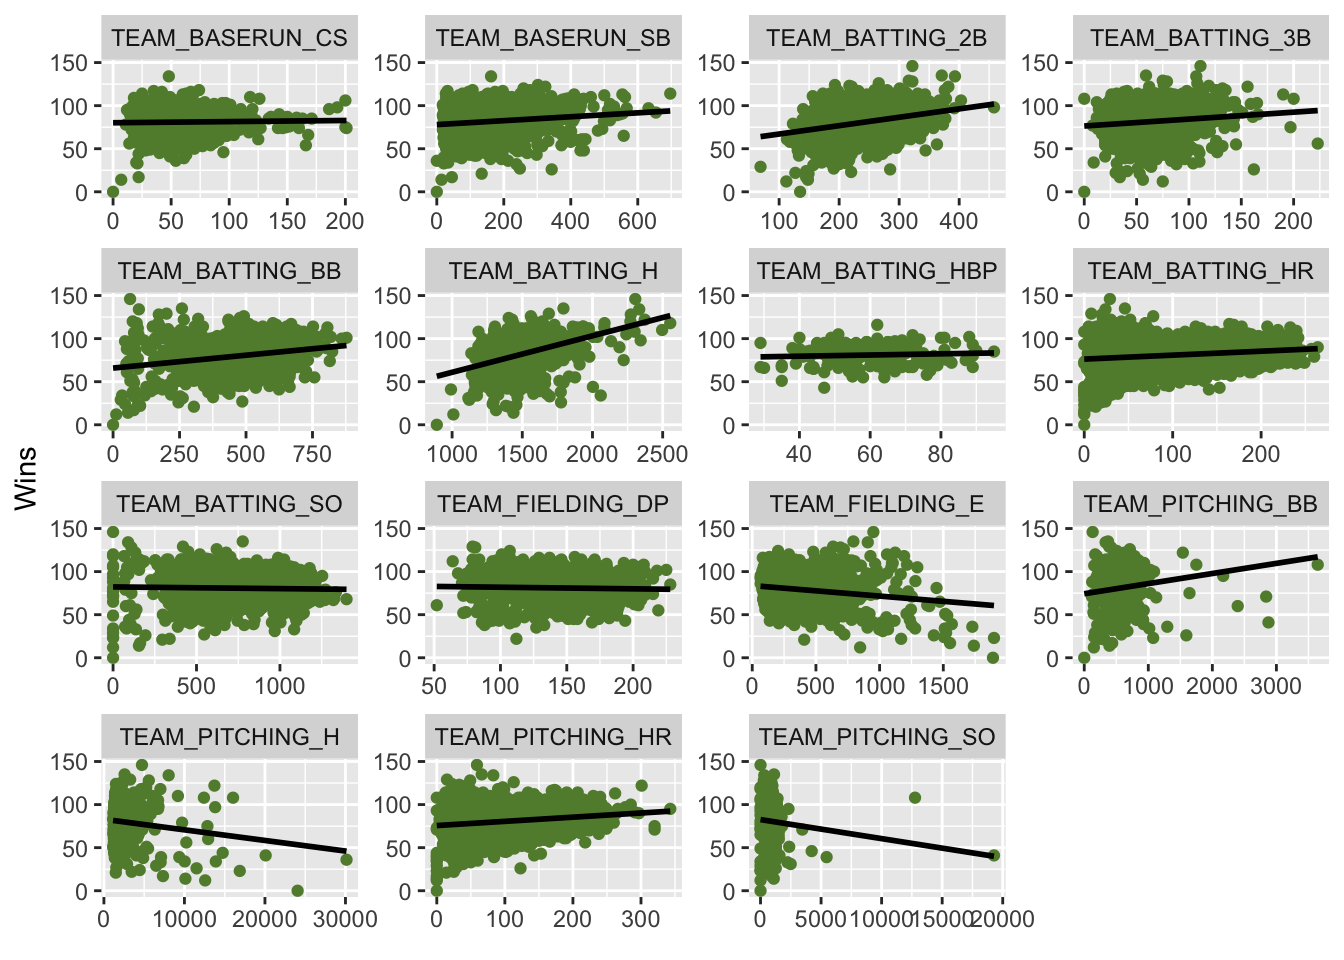
\includegraphics{Assignment1_Data621_HW_files/figure-latex/unnamed-chunk-3-1.pdf}

The Box Plot for Outlier Detection \& Distribution Analysis shows an
Interquartile Range - IQR with a range roughly from 70 to 92 wins.

The Box Plot suggests that there are several small circles (outliers)
below the lower whisker. Additionally, there are some outliers above the
upper whisker, but visually fewer than the low-end.

Since The TARGET\_WINS column has missing values, we should remove those
rows since we can't predict missing outcomes. Similarly, if it has a
zero (0) value, we may also want to drop this row, as it is highly
suspicious that a team would have 0 wins in 162 games.

\begin{Shaded}
\begin{Highlighting}[]
\NormalTok{train\_df }\OtherTok{\textless{}{-}}\NormalTok{ train\_df }\SpecialCharTok{\%\textgreater{}\%} 
  \FunctionTok{filter}\NormalTok{(}\SpecialCharTok{!}\FunctionTok{is.na}\NormalTok{(TARGET\_WINS) }\SpecialCharTok{\&}\NormalTok{ TARGET\_WINS }\SpecialCharTok{\textgreater{}}\DecValTok{0}\NormalTok{)}
\end{Highlighting}
\end{Shaded}

\paragraph{2. Missing Values}\label{missing-values}

Some variables have a significant number of missing values. In
particular:

\begin{itemize}
\tightlist
\item
  TEAM\_BATTING\_HBP (2085 missing values) \textless- very unreliable
\item
  TEAM\_BASERUN\_CS (772 missing values) \textless- potentially
  unreliable
\item
  TEAM\_BATTING\_SO (102 missing values)
\item
  TEAM\_BASERUN\_SB (131 missing values)
\item
  TEAM\_PITCHING\_SO (102 missing values)
\item
  TEAM\_FIELDING\_DP (286 missing values)
\end{itemize}

Additionally, four variables have values of zero (0) reported that
appear suspicious. In particular: - TEAM\_BATTING\_SO \&
TEAM\_PITHCING\_SO have the same rows entered as zero suggesting that
data may not have been available for these entries. - TEAM\_BATTING\_HR
\& TEAM\_PITHCING\_HR have the same rows entered as zero suggesting that
data may not have been available for these entries.

\emph{Actionable Steps:} - Removing TEAM\_BATTING\_HBP since most of
it's values are missing. - Impute missing values (later on).

\begin{Shaded}
\begin{Highlighting}[]
\NormalTok{train\_df }\OtherTok{\textless{}{-}}\NormalTok{ train\_df[, }\SpecialCharTok{!}\FunctionTok{names}\NormalTok{(train\_df) }\SpecialCharTok{\%in\%} \StringTok{"TEAM\_BATTING\_HBP"}\NormalTok{]}
\end{Highlighting}
\end{Shaded}

\subsubsection{Faceted Scatter Plot with Linear Regression
Lines:}\label{faceted-scatter-plot-with-linear-regression-lines}

These scatter plots give us a sense of the relationship between the each
variable and TARGET\_WINS. Data points are plotted where the x-axis
represents the predictor variable, and the y-axis represents the number
of wins. A black trend line is fitted using linear regression to show
the general direction and strength of the relationship between each
variable and TARGET\_WINS.

\begin{Shaded}
\begin{Highlighting}[]
\NormalTok{train\_df }\SpecialCharTok{\%\textgreater{}\%}
  \FunctionTok{gather}\NormalTok{(variable, value, }\SpecialCharTok{{-}}\NormalTok{TARGET\_WINS) }\SpecialCharTok{\%\textgreater{}\%}
  \FunctionTok{ggplot}\NormalTok{(., }\FunctionTok{aes}\NormalTok{(value, TARGET\_WINS)) }\SpecialCharTok{+} 
  \FunctionTok{geom\_point}\NormalTok{(}\AttributeTok{fill =} \StringTok{"\#628B3A"}\NormalTok{, }\AttributeTok{color=}\StringTok{"\#628B3A"}\NormalTok{)  }\SpecialCharTok{+} 
  \FunctionTok{geom\_smooth}\NormalTok{(}\AttributeTok{method =} \StringTok{"lm"}\NormalTok{, }\AttributeTok{se =} \ConstantTok{FALSE}\NormalTok{, }\AttributeTok{color =} \StringTok{"black"}\NormalTok{) }\SpecialCharTok{+} 
  \FunctionTok{facet\_wrap}\NormalTok{(}\SpecialCharTok{\textasciitilde{}}\NormalTok{variable, }\AttributeTok{scales =}\StringTok{"free"}\NormalTok{, }\AttributeTok{ncol =} \DecValTok{4}\NormalTok{) }\SpecialCharTok{+}
  \FunctionTok{labs}\NormalTok{(}\AttributeTok{x =} \FunctionTok{element\_blank}\NormalTok{(), }\AttributeTok{y =} \StringTok{"Wins"}\NormalTok{)}
\end{Highlighting}
\end{Shaded}

\begin{verbatim}
## `geom_smooth()` using formula = 'y ~ x'
\end{verbatim}

\begin{verbatim}
## Warning: Removed 1392 rows containing non-finite outside the scale range
## (`stat_smooth()`).
\end{verbatim}

\begin{verbatim}
## Warning: Removed 1392 rows containing missing values or values outside the scale range
## (`geom_point()`).
\end{verbatim}

\includegraphics{Assignment1_Data621_HW_files/figure-latex/unnamed-chunk-6-1.pdf}

The slope of the regression line in each facet is used to determine the
strength of relationship between the independent variable represent on
the x-axis vs the dependent variable y (TARGET\_WINS). The steeper the
slope, the stronger the relationship is between the two variables. The
direction of the slope tells whether the relationship is positive or
negative: - if the line is sloped to the right, it is a positive
relationship meaning we can expect an increase in y as x increases - if
the line is sloped to the left, it is a negative relationship meaning we
can expect an decrease in y as x increases - if the trend line is flat,
there is likely no meaningful relationship between that variable and
TARGET\_WINS.

If the points are closely clustered around the line, it suggests a
stronger linear relationship. If the points are widely scattered, the
variable may not strongly predict TARGET\_WINS.

\emph{Positive Predictors of Wins:} TEAM\_BATTING\_2B,
TEAM\_BATTING\_BB, TEAM\_BATTING\_H, TEAM\_PITCHING\_BB (unexpected).

\emph{Negative Predictors of Wins:} TEAM\_FIELDING\_E,
TEAM\_PITCHING\_H, TEAM\_PITCHING\_SO.

\emph{Weak or No Influence:} TEAM\_BATTING\_3B, TEAM\_BATTING\_SO,
TEAM\_FIELDING\_DP, TEAM\_PITCHING\_HR, , TEAM\_BATTING\_HBP (Removed).

\subsubsection{Correlations}\label{correlations}

In this section, we examine two different types of correlations: -
correlation between dependent and independent variables - correlation
between all variables

\paragraph{Correlation Between Dependent and Independent
variables}\label{correlation-between-dependent-and-independent-variables}

The correlation between the dependent variable TARGET\_WINS and each of
the independent variables. In this context, correlation pertains to the
strength (0:1) and direction (+/-) of the relationship between the
dependent and independent variable. A higher strength is indicated by a
number closer to 1 and describes a greater change on the dependent
variable by the independent variable. The direction describes whether
the change is increasing (positive) or decreasing (negative). The chart
below suggest that there is a relatively weak relationship between the
TARGET\_WINS and TEAM\_BASERUN\_SB and should be considered for omission
from our models.

\begin{Shaded}
\begin{Highlighting}[]
\NormalTok{correlation\_with\_target }\OtherTok{\textless{}{-}} \FunctionTok{cor}\NormalTok{(train\_df, }\AttributeTok{use =} \StringTok{"complete.obs"}\NormalTok{)[}\StringTok{"TARGET\_WINS"}\NormalTok{, ] }\SpecialCharTok{\%\textgreater{}\%}
  \FunctionTok{sort}\NormalTok{(}\AttributeTok{decreasing =} \ConstantTok{TRUE}\NormalTok{)  }\CommentTok{\# Sort from highest to lowest correlation}

\NormalTok{correlation\_data }\OtherTok{\textless{}{-}} \FunctionTok{data.frame}\NormalTok{(}\AttributeTok{Variable =} \FunctionTok{names}\NormalTok{(correlation\_with\_target), }\AttributeTok{Correlation =}\NormalTok{ correlation\_with\_target)}

\FunctionTok{ggplot}\NormalTok{(correlation\_data, }\FunctionTok{aes}\NormalTok{(}\AttributeTok{x =} \FunctionTok{reorder}\NormalTok{(Variable, Correlation), }\AttributeTok{y =}\NormalTok{ Correlation, }\AttributeTok{fill =}\NormalTok{ Correlation }\SpecialCharTok{\textgreater{}} \DecValTok{0}\NormalTok{)) }\SpecialCharTok{+}
  \FunctionTok{geom\_bar}\NormalTok{(}\AttributeTok{stat =} \StringTok{"identity"}\NormalTok{) }\SpecialCharTok{+}
  \FunctionTok{coord\_flip}\NormalTok{() }\SpecialCharTok{+}  \CommentTok{\# Flip for better readability}
  \FunctionTok{labs}\NormalTok{(}\AttributeTok{title =} \StringTok{"Correlation with Target Wins"}\NormalTok{, }\AttributeTok{x =} \StringTok{"Variables"}\NormalTok{, }\AttributeTok{y =} \StringTok{"Correlation"}\NormalTok{) }\SpecialCharTok{+}
  \FunctionTok{scale\_fill\_manual}\NormalTok{(}\AttributeTok{values =} \FunctionTok{c}\NormalTok{(}\StringTok{"red"}\NormalTok{, }\StringTok{"blue"}\NormalTok{)) }\SpecialCharTok{+}
  \FunctionTok{theme\_minimal}\NormalTok{()}
\end{Highlighting}
\end{Shaded}

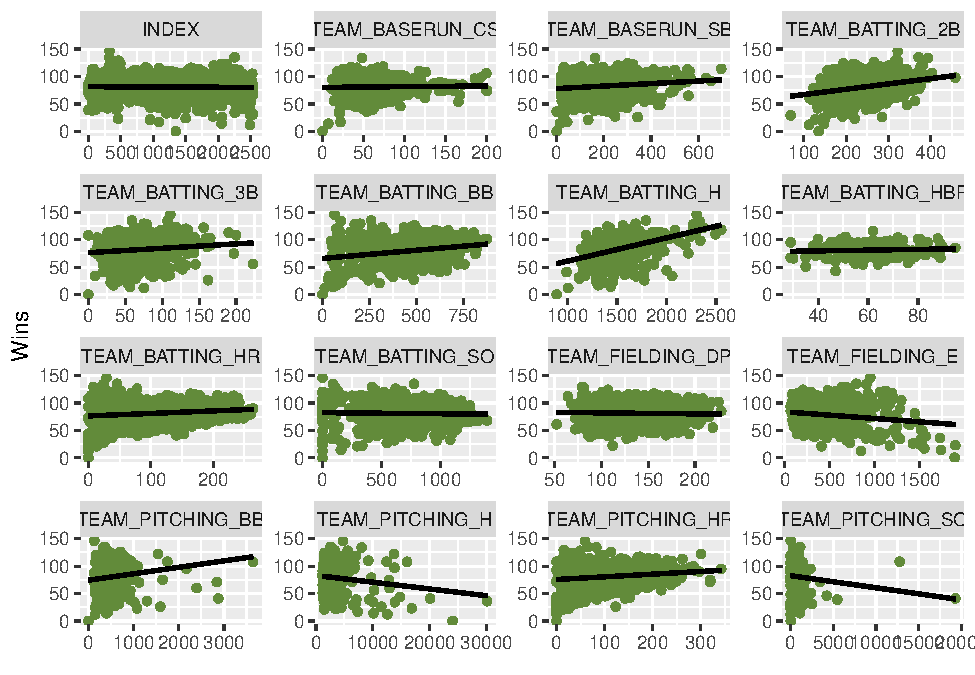
\includegraphics{Assignment1_Data621_HW_files/figure-latex/unnamed-chunk-7-1.pdf}

\paragraph{Correlation Between All
Variables}\label{correlation-between-all-variables}

Testing the correlation between all variables shows how the change in
one variable affects the change in another. In this case, a high
correlation value between two independent variables, regardless of
direction, suggests multicollinearity between the variables meaning that
they are not independent from one another and thus breaks our assumption
of independence.

\begin{Shaded}
\begin{Highlighting}[]
\NormalTok{cor\_matrix }\OtherTok{\textless{}{-}} \FunctionTok{cor}\NormalTok{(train\_df, }\AttributeTok{use =} \StringTok{"complete.obs"}\NormalTok{)}
\NormalTok{cor\_df }\OtherTok{\textless{}{-}} \FunctionTok{as.data.frame}\NormalTok{(}\FunctionTok{as.table}\NormalTok{(cor\_matrix))}
\NormalTok{cor\_df }\OtherTok{\textless{}{-}}\NormalTok{ cor\_df[cor\_df}\SpecialCharTok{$}\NormalTok{Var1 }\SpecialCharTok{!=}\NormalTok{ cor\_df}\SpecialCharTok{$}\NormalTok{Var2, ]}
\NormalTok{cor\_df }\OtherTok{\textless{}{-}}\NormalTok{ cor\_df[}\FunctionTok{order}\NormalTok{(cor\_df}\SpecialCharTok{$}\NormalTok{Freq, }\AttributeTok{decreasing =} \ConstantTok{TRUE}\NormalTok{), ]}
\end{Highlighting}
\end{Shaded}

The correlation matrix shows that the following variables are very
highly correlated with one another:

\emph{Top 3 Positive Correlation}

\begin{Shaded}
\begin{Highlighting}[]
\FunctionTok{head}\NormalTok{(cor\_df, }\DecValTok{3}\NormalTok{)}
\end{Highlighting}
\end{Shaded}

\begin{verbatim}
##                 Var1             Var2      Freq
## 71  TEAM_PITCHING_HR  TEAM_BATTING_HR 0.9716522
## 155  TEAM_BATTING_HR TEAM_PITCHING_HR 0.9716522
## 103 TEAM_PITCHING_SO  TEAM_BATTING_SO 0.9322116
\end{verbatim}

\emph{Top 3 Negative Correlation}

\begin{Shaded}
\begin{Highlighting}[]
\FunctionTok{head}\NormalTok{(cor\_df[}\FunctionTok{order}\NormalTok{(cor\_df}\SpecialCharTok{$}\NormalTok{Freq), ], }\DecValTok{3}\NormalTok{)}
\end{Highlighting}
\end{Shaded}

\begin{verbatim}
##                Var1            Var2       Freq
## 52  TEAM_BATTING_SO TEAM_BATTING_3B -0.6903472
## 94  TEAM_BATTING_3B TEAM_BATTING_SO -0.6903472
## 58 TEAM_PITCHING_SO TEAM_BATTING_3B -0.6392928
\end{verbatim}

\subsubsection{Potential Outliers \& Data
Issues}\label{potential-outliers-data-issues}

We observed the following the following values that seem suspicious:

\begin{itemize}
\tightlist
\item
  TEAM\_PITCHING\_H (Max = 30,132) \textless- Likely an error since
  typical values range from 1,200 - 1,700.
\item
  TEAM\_PITCHING\_SO (Max = 19,278) \textless- Suspiciously high
  (typical range: 500 - 1,500).
\item
  TEAM\_PITCHING\_BB (Max = 3,645) \textless- Very high (typical range:
  300 - 700).
\item
  TEAM\_FIELDING\_E (Max = 1,898) \textless- Likely an error since the
  normal range is \textasciitilde{} 70-200.
\end{itemize}

We will take a look at only potential outliers that have a significant
leverage when we start fitting our model.

\subsection{Section 3: Data
Preparation}\label{section-3-data-preparation}

Before fitting our model, we will consider the following data cleaning
steps:

\begin{itemize}
\item
  Consider dropping or imputing variables with too many missing values
  (e.g., TEAM\_BATTING\_HBP).
\item
  Remove or Adjust Extreme Outliers
\end{itemize}

Once cleaned, feature selection and multicollinearity checks will be
essential to ensure a robust and interpretable model for predicting team
wins.

\paragraph{Identifying Missing Values}\label{identifying-missing-values}

We previously identified several variables with many missing fields. Our
first step was to drop \emph{TEAM\_BATTING\_HBP} as most of its values
were missing. In this next section, we will address the following
missing values

\begin{Shaded}
\begin{Highlighting}[]
\NormalTok{missing\_values }\OtherTok{\textless{}{-}}\NormalTok{ train\_df }\SpecialCharTok{\%\textgreater{}\%}
  \FunctionTok{summarise}\NormalTok{(}\FunctionTok{across}\NormalTok{(}\FunctionTok{everything}\NormalTok{(), }\SpecialCharTok{\textasciitilde{}} \FunctionTok{sum}\NormalTok{(}\FunctionTok{is.na}\NormalTok{(.)))) }\SpecialCharTok{\%\textgreater{}\%}
  \FunctionTok{pivot\_longer}\NormalTok{(}\AttributeTok{cols =} \FunctionTok{everything}\NormalTok{(), }\AttributeTok{names\_to =} \StringTok{"Variable"}\NormalTok{, }\AttributeTok{values\_to =} \StringTok{"Missing\_Count"}\NormalTok{) }\SpecialCharTok{\%\textgreater{}\%}
  \FunctionTok{filter}\NormalTok{(Missing\_Count }\SpecialCharTok{\textgreater{}} \DecValTok{0}\NormalTok{) }\SpecialCharTok{\%\textgreater{}\%}
  \FunctionTok{arrange}\NormalTok{(}\FunctionTok{desc}\NormalTok{(Missing\_Count))}

\FunctionTok{print}\NormalTok{(missing\_values)}
\end{Highlighting}
\end{Shaded}

\begin{verbatim}
## # A tibble: 5 x 2
##   Variable         Missing_Count
##   <chr>                    <int>
## 1 TEAM_BASERUN_CS            772
## 2 TEAM_FIELDING_DP           285
## 3 TEAM_BASERUN_SB            131
## 4 TEAM_BATTING_SO            102
## 5 TEAM_PITCHING_SO           102
\end{verbatim}

The variables \emph{TEAM\_BATTING\_SO}, \emph{TEAM\_PITCHING\_SO},
\emph{TEAM\_BATTING\_HR}, and \emph{TEAM\_PITCHING\_HR} included several
observations with a value of zero. As the rows were the same for both
variables, it appears that these may also be missing observations as the
likelihood that a team's batters did not have a single strikeout nor did
their pitchers pitch a single strikeout over the course of a 162 game
season is highly unlikely. We will therefore treat these as missing
observations and impute using the median value which is more robust to
outliers then using the mean values. We will also drop the single row
where the team did not win a single game, as this is also suspicious.

\paragraph{Handling Missing Values}\label{handling-missing-values}

Next, we will address the remaining missing values. We will weight
several options:

\subparagraph{Removing Missing Values}\label{removing-missing-values}

Dropping missing values could result in significantly reducing the
sample size and thus the predictive power of your model. It can also
introduce bias if the missing data is not missing completely at random
(MCAR) or if too many observations are dropped from certain categories.
We will therefore explore other methods.

\subparagraph{Mean Imputation}\label{mean-imputation}

Mean imputation makes the imputed values less variable and could lead to
an underestimation of the variability in your model. It may also
over-simplify the observations and create artificial relationships. It
can also introduce bias if the missing data is not missing completely at
random (MCAR) or if too many observations are dropped from certain
categories.

\subparagraph{Median Imputation}\label{median-imputation}

Median imputation has many of the same issues as mean imputation but is
more robust to the effects of skewing and outliers. However, it can also
introduce bias if the missing data is not missing completely at random
(MCAR) or if too many observations are dropped from certain categories.

\subparagraph{Regression Imputation}\label{regression-imputation}

Regression Imputation uses predictive models to predict missing values
based on our dataframe and is one of the suggested techniques for values
Missing at Random (MAR). However, if data is not Missing at Random
(MAR), we can inadvertently introduce bias in our data.

\subparagraph{Imputing}\label{imputing}

Upon further analysis, we noticed a pattern between 4 parameters with
missing values: TEAM\_BATTING\_SO, TEAM\_PITCHING\_SO,
TEAM\_BATTING\_HR, and TEAM\_PITCHING\_HR suggesting that these missing
values may be MAR. However, no pattern was evident for the other three
parameters with missing values (TEAM\_BASERUN\_CS, TEAM\_FIELDING\_DP,
TEAM\_BASERUN\_SB) suggesting that we they may be MCAR. As such, we
should apply two separate techniques for the missing values suitable for
their specific classification.Specifically, we will apply:

\begin{itemize}
\tightlist
\item
  Median imputation to TEAM\_BASERUN\_CS, TEAM\_FIELDING\_DP,
  TEAM\_BASERUN\_SB as it is a more robust form of imputation for MCAR
  values than mean imputation which is more affected by outliers
\item
  MICE imputation to TEAM\_BATTING\_SO, TEAM\_PITCHING\_SO,
  TEAM\_BATTING\_HR, and TEAM\_PITCHING\_HR as it as more robust method
  for MAR values.
\end{itemize}

\begin{Shaded}
\begin{Highlighting}[]
\FunctionTok{library}\NormalTok{(miscTools)}

\NormalTok{train\_df\_median }\OtherTok{\textless{}{-}}\NormalTok{ train\_df}
\NormalTok{median\_val }\OtherTok{\textless{}{-}} \FunctionTok{colMedians}\NormalTok{(train\_df\_median, }\AttributeTok{na.rm =} \ConstantTok{TRUE}\NormalTok{)}

\CommentTok{\# Impute using medians}
\ControlFlowTok{for}\NormalTok{(i }\ControlFlowTok{in} \FunctionTok{c}\NormalTok{(}\StringTok{\textquotesingle{}TEAM\_BASERUN\_CS\textquotesingle{}}\NormalTok{,   }\StringTok{\textquotesingle{}TEAM\_FIELDING\_DP\textquotesingle{}}\NormalTok{, }\StringTok{\textquotesingle{}TEAM\_BASERUN\_SB\textquotesingle{}}\NormalTok{))}
\NormalTok{    train\_df\_median[,i][}\FunctionTok{is.na}\NormalTok{(train\_df\_median[,i])] }\OtherTok{\textless{}{-}}\NormalTok{ median\_val[i]}
\end{Highlighting}
\end{Shaded}

\begin{Shaded}
\begin{Highlighting}[]
\CommentTok{\# Convert dubious stats to NAs for pitching}
\CommentTok{\# and drop unnecessary columns}
\NormalTok{train\_df\_median }\OtherTok{\textless{}{-}}\NormalTok{ train\_df\_median }\SpecialCharTok{|\textgreater{}}
  \FunctionTok{mutate}\NormalTok{(}
    \AttributeTok{TEAM\_BATTING\_SO =} \FunctionTok{if\_else}\NormalTok{(TEAM\_BATTING\_SO }\SpecialCharTok{\textgreater{}} \DecValTok{0}\NormalTok{, TEAM\_BATTING\_SO, }\ConstantTok{NA\_integer\_}\NormalTok{),}
    \AttributeTok{TEAM\_PITCHING\_SO =} \FunctionTok{if\_else}\NormalTok{(TEAM\_PITCHING\_SO }\SpecialCharTok{\textgreater{}} \DecValTok{0}\NormalTok{, TEAM\_PITCHING\_SO, }\ConstantTok{NA\_integer\_}\NormalTok{),}
    \AttributeTok{TEAM\_BATTING\_HR =} \FunctionTok{if\_else}\NormalTok{(TEAM\_BATTING\_HR }\SpecialCharTok{\textgreater{}} \DecValTok{0}\NormalTok{, TEAM\_BATTING\_HR, }\ConstantTok{NA\_integer\_}\NormalTok{),}
    \AttributeTok{TEAM\_PITCHING\_HR =} \FunctionTok{if\_else}\NormalTok{(TEAM\_PITCHING\_HR }\SpecialCharTok{\textgreater{}} \DecValTok{0}\NormalTok{, TEAM\_PITCHING\_HR, }\ConstantTok{NA\_integer\_}\NormalTok{)}
\NormalTok{  ) }
\end{Highlighting}
\end{Shaded}

\begin{Shaded}
\begin{Highlighting}[]
\NormalTok{regimp }\OtherTok{\textless{}{-}} \FunctionTok{lm}\NormalTok{(TEAM\_BATTING\_SO }\SpecialCharTok{\textasciitilde{}}\NormalTok{ . }\SpecialCharTok{{-}}\NormalTok{ TEAM\_PITCHING\_SO }\SpecialCharTok{{-}}\NormalTok{ TEAM\_BATTING\_HR }\SpecialCharTok{{-}}\NormalTok{ TEAM\_PITCHING\_HR, }\AttributeTok{data =}\NormalTok{ train\_df\_median)}

\CommentTok{\# Predict missing values }
\NormalTok{train\_df\_median}\SpecialCharTok{$}\NormalTok{TEAM\_BATTING\_SO[}\FunctionTok{is.na}\NormalTok{(train\_df\_median}\SpecialCharTok{$}\NormalTok{TEAM\_BATTING\_SO)] }\OtherTok{\textless{}{-}} \FunctionTok{predict}\NormalTok{(regimp, }\AttributeTok{newdata =}\NormalTok{ train\_df\_median[}\FunctionTok{is.na}\NormalTok{(train\_df\_median}\SpecialCharTok{$}\NormalTok{TEAM\_BATTING\_SO), ])}

\NormalTok{regimp }\OtherTok{\textless{}{-}} \FunctionTok{lm}\NormalTok{(TEAM\_PITCHING\_SO }\SpecialCharTok{\textasciitilde{}}\NormalTok{ . }\SpecialCharTok{{-}}\NormalTok{ TEAM\_BATTING\_SO }\SpecialCharTok{{-}}\NormalTok{ TEAM\_BATTING\_HR }\SpecialCharTok{{-}}\NormalTok{ TEAM\_PITCHING\_HR, }\AttributeTok{data =}\NormalTok{ train\_df\_median)}

\CommentTok{\# Predict missing values }
\NormalTok{train\_df\_median}\SpecialCharTok{$}\NormalTok{TEAM\_PITCHING\_SO[}\FunctionTok{is.na}\NormalTok{(train\_df\_median}\SpecialCharTok{$}\NormalTok{TEAM\_PITCHING\_SO)] }\OtherTok{\textless{}{-}} \FunctionTok{predict}\NormalTok{(regimp, }\AttributeTok{newdata =}\NormalTok{ train\_df\_median[}\FunctionTok{is.na}\NormalTok{(train\_df\_median}\SpecialCharTok{$}\NormalTok{TEAM\_PITCHING\_SO), ])}

\NormalTok{regimp }\OtherTok{\textless{}{-}} \FunctionTok{lm}\NormalTok{(TEAM\_BATTING\_HR }\SpecialCharTok{\textasciitilde{}}\NormalTok{ . }\SpecialCharTok{{-}}\NormalTok{ TEAM\_PITCHING\_SO }\SpecialCharTok{{-}}\NormalTok{ TEAM\_BATTING\_SO }\SpecialCharTok{{-}}\NormalTok{ TEAM\_PITCHING\_HR, }\AttributeTok{data =}\NormalTok{ train\_df\_median)}

\CommentTok{\# Predict missing values }
\NormalTok{train\_df\_median}\SpecialCharTok{$}\NormalTok{TEAM\_BATTING\_HR[}\FunctionTok{is.na}\NormalTok{(train\_df\_median}\SpecialCharTok{$}\NormalTok{TEAM\_BATTING\_HR)] }\OtherTok{\textless{}{-}} \FunctionTok{predict}\NormalTok{(regimp, }\AttributeTok{newdata =}\NormalTok{ train\_df\_median[}\FunctionTok{is.na}\NormalTok{(train\_df\_median}\SpecialCharTok{$}\NormalTok{TEAM\_BATTING\_HR), ])}

\NormalTok{regimp }\OtherTok{\textless{}{-}} \FunctionTok{lm}\NormalTok{(TEAM\_PITCHING\_HR }\SpecialCharTok{\textasciitilde{}}\NormalTok{ . }\SpecialCharTok{{-}}\NormalTok{ TEAM\_PITCHING\_SO }\SpecialCharTok{{-}}\NormalTok{ TEAM\_BATTING\_SO }\SpecialCharTok{{-}}\NormalTok{ TEAM\_BATTING\_HR, }\AttributeTok{data =}\NormalTok{ train\_df\_median)}

\CommentTok{\# Predict missing values }
\NormalTok{train\_df\_median}\SpecialCharTok{$}\NormalTok{TEAM\_PITCHING\_HR[}\FunctionTok{is.na}\NormalTok{(train\_df\_median}\SpecialCharTok{$}\NormalTok{TEAM\_PITCHING\_HR)] }\OtherTok{\textless{}{-}} \FunctionTok{predict}\NormalTok{(regimp, }\AttributeTok{newdata =}\NormalTok{ train\_df\_median[}\FunctionTok{is.na}\NormalTok{(train\_df\_median}\SpecialCharTok{$}\NormalTok{TEAM\_PITCHING\_HR), ])}

\NormalTok{train\_df\_clean }\OtherTok{\textless{}{-}}\NormalTok{ train\_df\_median }\SpecialCharTok{|\textgreater{}}
  \FunctionTok{filter}\NormalTok{(}\SpecialCharTok{!}\NormalTok{TEAM\_BATTING\_HR }\SpecialCharTok{\textless{}} \DecValTok{0}\NormalTok{)}

\FunctionTok{print}\NormalTok{(}\FunctionTok{colSums}\NormalTok{(}\FunctionTok{is.na}\NormalTok{(train\_df\_clean)))}
\end{Highlighting}
\end{Shaded}

\begin{verbatim}
##      TARGET_WINS   TEAM_BATTING_H  TEAM_BATTING_2B  TEAM_BATTING_3B 
##                0                0                0                0 
##  TEAM_BATTING_HR  TEAM_BATTING_BB  TEAM_BATTING_SO  TEAM_BASERUN_SB 
##                0                0                0                0 
##  TEAM_BASERUN_CS  TEAM_PITCHING_H TEAM_PITCHING_HR TEAM_PITCHING_BB 
##                0                0                0                0 
## TEAM_PITCHING_SO  TEAM_FIELDING_E TEAM_FIELDING_DP 
##                0                0                0
\end{verbatim}

\subsubsection{Splitting the training
dataset}\label{splitting-the-training-dataset}

We split the original training dataset into a training and testing
dataset in order to test the strength of our model without testing the
model on data that the model has already seen. The training dataset will
contain 75\% randomly selected observations from our original dataset of
2276 observations, while the test dataset will hold 25\%. Some potential
drawbacks of this technique are that we will make our sample size
smaller, which may negatively affect our model if our sample size is
small. As our split training set will still contain 1706 observations,
it should still provide an adequate sample size. We also explore
Cross-Validation techniques later on in our analysis.

\begin{Shaded}
\begin{Highlighting}[]
\NormalTok{smp\_size }\OtherTok{\textless{}{-}} \FunctionTok{floor}\NormalTok{(}\FloatTok{0.75} \SpecialCharTok{*} \FunctionTok{nrow}\NormalTok{(train\_df\_clean))}
 \FunctionTok{nrow}\NormalTok{(train\_df\_clean)}
\end{Highlighting}
\end{Shaded}

\begin{verbatim}
## [1] 2272
\end{verbatim}

\begin{Shaded}
\begin{Highlighting}[]
\DocumentationTok{\#\# set the seed to make your partition reproducible}
\FunctionTok{set.seed}\NormalTok{(}\DecValTok{123}\NormalTok{)}
\NormalTok{train\_ind }\OtherTok{\textless{}{-}} \FunctionTok{sample}\NormalTok{(}\FunctionTok{seq\_len}\NormalTok{(}\FunctionTok{nrow}\NormalTok{(train\_df\_clean)), }\AttributeTok{size =}\NormalTok{ smp\_size)}

\NormalTok{stp75\_train\_df }\OtherTok{\textless{}{-}}\NormalTok{ train\_df\_clean[train\_ind, ]}
\NormalTok{stp25\_test\_df }\OtherTok{\textless{}{-}}\NormalTok{ train\_df\_clean[}\SpecialCharTok{{-}}\NormalTok{train\_ind, ]}
\end{Highlighting}
\end{Shaded}

\subsubsection{Handling Outliers}\label{handling-outliers}

The Residuals vs.~Fitted and QQ Plots show a fairly linear pattern,
while Scale-Location plot suggest Homoscedasticity. However, the
Residuals vs Leverage plot reveals the presence of some outliers.

\begin{Shaded}
\begin{Highlighting}[]
\NormalTok{stp\_model\_full }\OtherTok{\textless{}{-}} \FunctionTok{lm}\NormalTok{(TARGET\_WINS }\SpecialCharTok{\textasciitilde{}}\NormalTok{ ., }\AttributeTok{data =}\NormalTok{ stp75\_train\_df)}
\FunctionTok{summary}\NormalTok{(stp\_model\_full)}
\end{Highlighting}
\end{Shaded}

\begin{verbatim}
## 
## Call:
## lm(formula = TARGET_WINS ~ ., data = stp75_train_df)
## 
## Residuals:
##     Min      1Q  Median      3Q     Max 
## -49.368  -8.679   0.066   8.688  56.218 
## 
## Coefficients:
##                    Estimate Std. Error t value Pr(>|t|)    
## (Intercept)      20.4600045  6.3967791   3.198 0.001407 ** 
## TEAM_BATTING_H    0.0500658  0.0046097  10.861  < 2e-16 ***
## TEAM_BATTING_2B  -0.0155618  0.0107659  -1.445 0.148512    
## TEAM_BATTING_3B   0.0684310  0.0199331   3.433 0.000611 ***
## TEAM_BATTING_HR   0.0088616  0.0380506   0.233 0.815876    
## TEAM_BATTING_BB   0.0071417  0.0066875   1.068 0.285710    
## TEAM_BATTING_SO  -0.0050954  0.0029167  -1.747 0.080820 .  
## TEAM_BASERUN_SB   0.0272244  0.0049691   5.479 4.93e-08 ***
## TEAM_BASERUN_CS  -0.0167830  0.0178406  -0.941 0.346984    
## TEAM_PITCHING_H  -0.0013517  0.0005253  -2.573 0.010163 *  
## TEAM_PITCHING_HR  0.0481588  0.0343963   1.400 0.161663    
## TEAM_PITCHING_BB  0.0015495  0.0047460   0.326 0.744102    
## TEAM_PITCHING_SO  0.0017487  0.0009339   1.872 0.061321 .  
## TEAM_FIELDING_E  -0.0187658  0.0028495  -6.586 6.03e-11 ***
## TEAM_FIELDING_DP -0.1158577  0.0149777  -7.735 1.76e-14 ***
## ---
## Signif. codes:  0 '***' 0.001 '**' 0.01 '*' 0.05 '.' 0.1 ' ' 1
## 
## Residual standard error: 13.16 on 1689 degrees of freedom
## Multiple R-squared:  0.3059, Adjusted R-squared:  0.3001 
## F-statistic: 53.17 on 14 and 1689 DF,  p-value: < 2.2e-16
\end{verbatim}

\begin{Shaded}
\begin{Highlighting}[]
\CommentTok{\# check for outliers using cooks{-}distance plot}
\FunctionTok{plot}\NormalTok{(stp\_model\_full, }\AttributeTok{which =} \DecValTok{4}\NormalTok{,  }\AttributeTok{id.n =} \DecValTok{8}\NormalTok{)}
\end{Highlighting}
\end{Shaded}

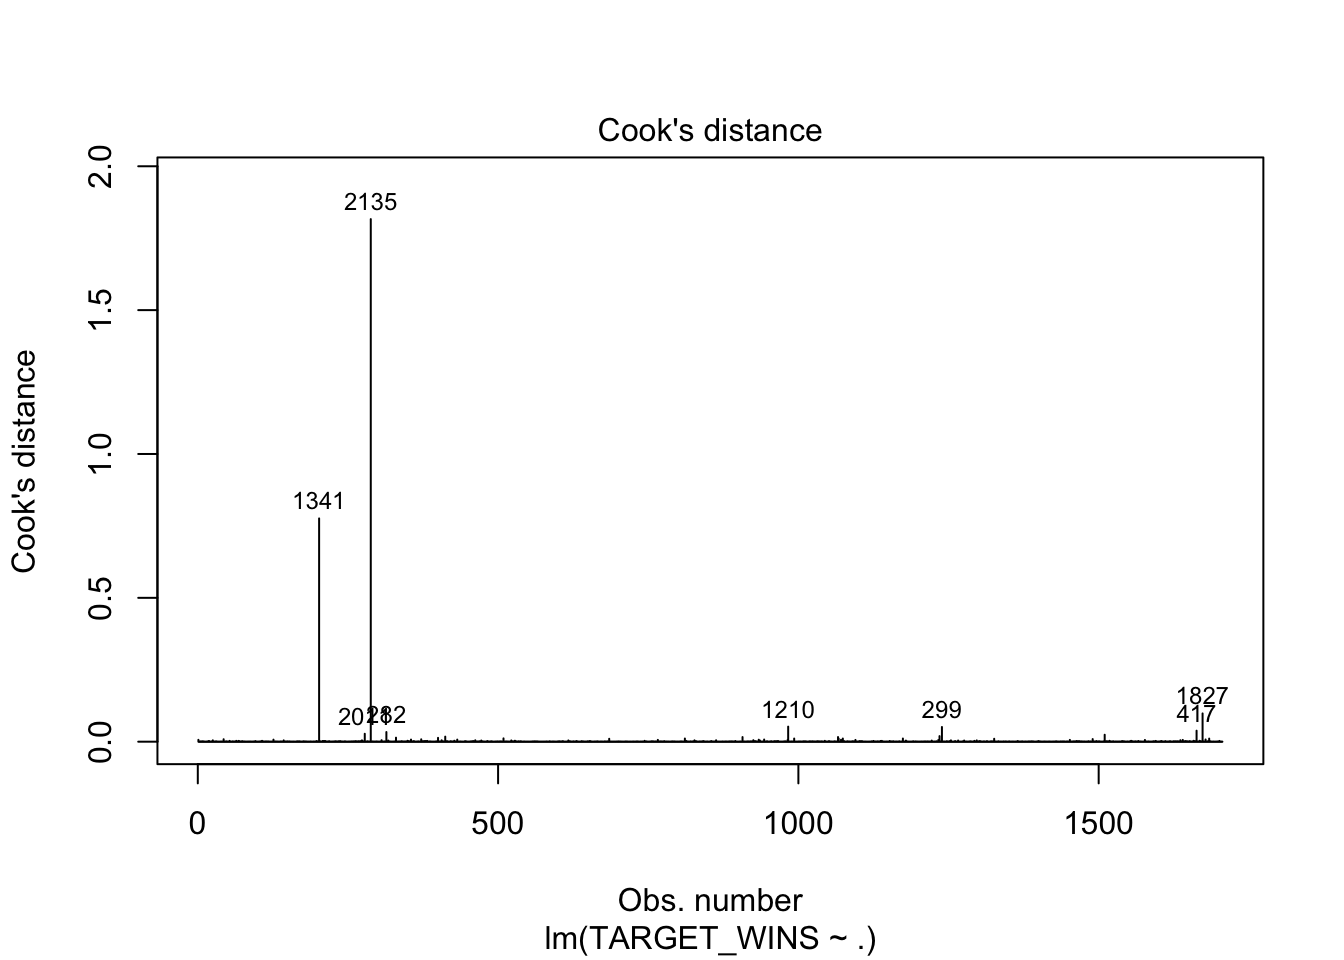
\includegraphics{Assignment1_Data621_HW_files/figure-latex/model4-full-1.pdf}

\begin{Shaded}
\begin{Highlighting}[]
\CommentTok{\# get points of influence}
\NormalTok{influence }\OtherTok{\textless{}{-}} \FunctionTok{influence.measures}\NormalTok{(stp\_model\_full)}
\NormalTok{influential\_points }\OtherTok{\textless{}{-}}\NormalTok{ influence}\SpecialCharTok{$}\NormalTok{infmat}
\NormalTok{cooks\_d }\OtherTok{\textless{}{-}}\NormalTok{ influence}\SpecialCharTok{$}\NormalTok{infmat[, }\StringTok{"cook.d"}\NormalTok{]}
\NormalTok{max\_influence\_index }\OtherTok{\textless{}{-}} \FunctionTok{which.max}\NormalTok{(cooks\_d)}
\end{Highlighting}
\end{Shaded}

The observation with index 2135 is particularly problematic. A closer
examination reveals \emph{TEAM\_PITCHING\_SO} is almost 75\% higher as
the next highest value (19278 vs 12758). \emph{TEAM\_PITCHING\_H} is
also unusually high for this year.

\begin{Shaded}
\begin{Highlighting}[]
\NormalTok{influential\_data\_point }\OtherTok{\textless{}{-}}\NormalTok{ stp75\_train\_df[max\_influence\_index, ]}
\FunctionTok{print}\NormalTok{(influential\_data\_point)}
\end{Highlighting}
\end{Shaded}

\begin{verbatim}
##      TARGET_WINS TEAM_BATTING_H TEAM_BATTING_2B TEAM_BATTING_3B TEAM_BATTING_HR
## 2134          41            992             263              20        99.83087
##      TEAM_BATTING_BB TEAM_BATTING_SO TEAM_BASERUN_SB TEAM_BASERUN_CS
## 2134             142             952             101              49
##      TEAM_PITCHING_H TEAM_PITCHING_HR TEAM_PITCHING_BB TEAM_PITCHING_SO
## 2134           20088         407.0946             2876            19278
##      TEAM_FIELDING_E TEAM_FIELDING_DP
## 2134             952              149
\end{verbatim}

We will drop this row since it has such a high leverage on the model.

\begin{Shaded}
\begin{Highlighting}[]
\CommentTok{\# remove outlier }
\NormalTok{stp75\_train\_df }\OtherTok{\textless{}{-}}\NormalTok{ stp75\_train\_df }\SpecialCharTok{|\textgreater{}}
  \FunctionTok{filter}\NormalTok{(TEAM\_PITCHING\_SO }\SpecialCharTok{\textless{}} \DecValTok{15000}\NormalTok{)}

\CommentTok{\# confirm outliers}
\NormalTok{stp\_model\_full }\OtherTok{\textless{}{-}} \FunctionTok{lm}\NormalTok{(TARGET\_WINS }\SpecialCharTok{\textasciitilde{}}\NormalTok{ ., }\AttributeTok{data =}\NormalTok{ stp75\_train\_df)}
\FunctionTok{plot}\NormalTok{(stp\_model\_full, }\AttributeTok{which =} \DecValTok{4}\NormalTok{,  }\AttributeTok{id.n =} \DecValTok{8}\NormalTok{)}
\end{Highlighting}
\end{Shaded}

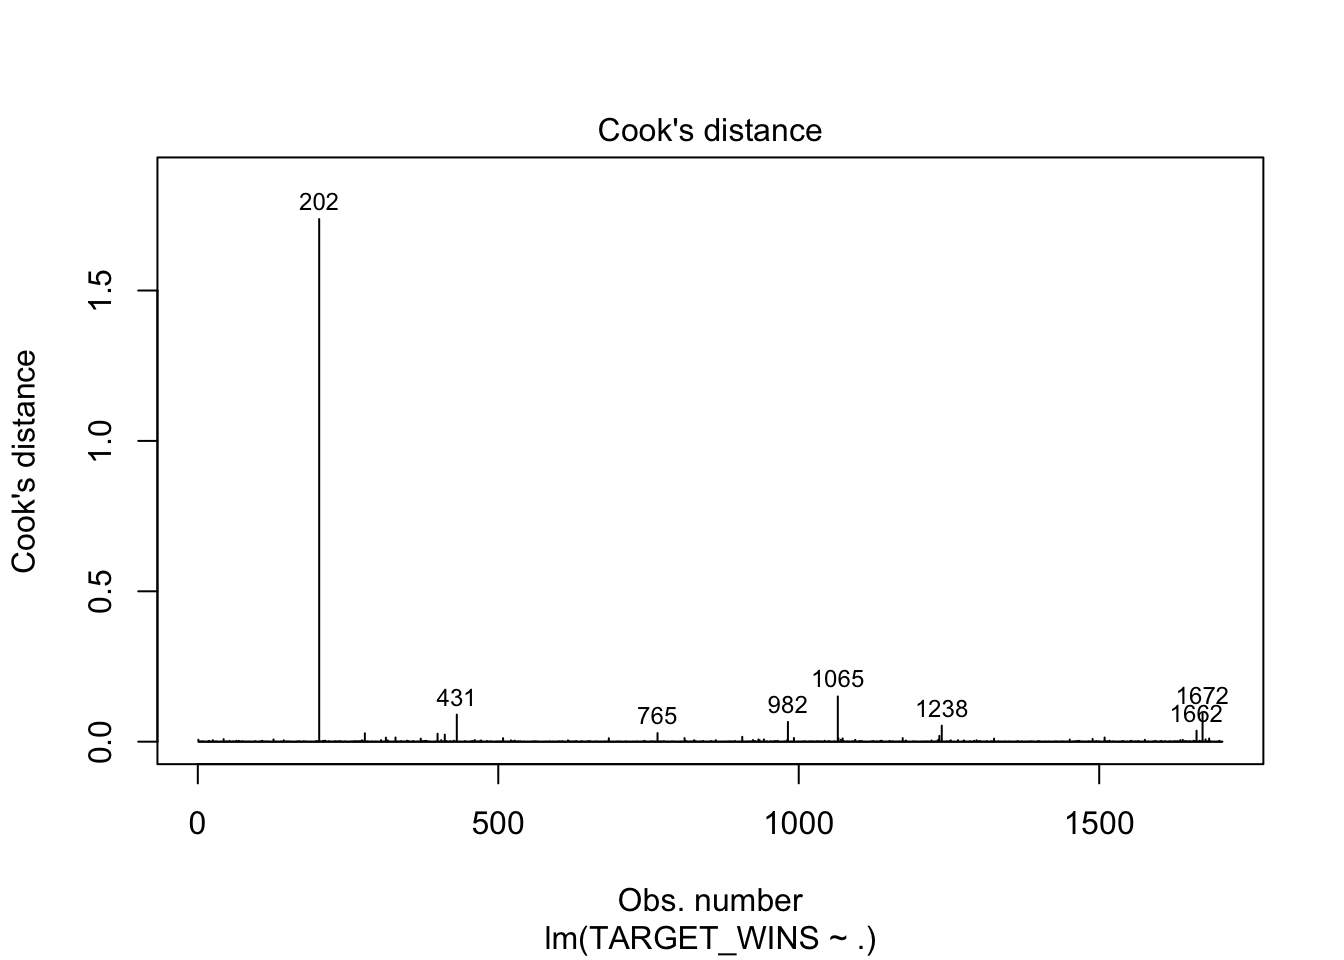
\includegraphics{Assignment1_Data621_HW_files/figure-latex/model4-drop-outlier-2135-1.pdf}

Charting the plot shows another point (202) with high influence. This
record has a TEAM\_PITCHING\_SO that is more than twice the next closest
value.

\begin{Shaded}
\begin{Highlighting}[]
\CommentTok{\# get points of influence}
\NormalTok{influence }\OtherTok{\textless{}{-}} \FunctionTok{influence.measures}\NormalTok{(stp\_model\_full)}
\NormalTok{influential\_points }\OtherTok{\textless{}{-}}\NormalTok{ influence}\SpecialCharTok{$}\NormalTok{infmat}
\NormalTok{cooks\_d }\OtherTok{\textless{}{-}}\NormalTok{ influence}\SpecialCharTok{$}\NormalTok{infmat[, }\StringTok{"cook.d"}\NormalTok{]}
\NormalTok{max\_influence\_index }\OtherTok{\textless{}{-}} \FunctionTok{which.max}\NormalTok{(cooks\_d)}
\NormalTok{influential\_data\_point }\OtherTok{\textless{}{-}}\NormalTok{ stp75\_train\_df[max\_influence\_index, ]}
\FunctionTok{print}\NormalTok{(influential\_data\_point)}
\end{Highlighting}
\end{Shaded}

\begin{verbatim}
##     TARGET_WINS TEAM_BATTING_H TEAM_BATTING_2B TEAM_BATTING_3B TEAM_BATTING_HR
## 202         108           1188             338               0        159.8919
##     TEAM_BATTING_BB TEAM_BATTING_SO TEAM_BASERUN_SB TEAM_BASERUN_CS
## 202             270             945             101              49
##     TEAM_PITCHING_H TEAM_PITCHING_HR TEAM_PITCHING_BB TEAM_PITCHING_SO
## 202           16038         490.5011             3645            12758
##     TEAM_FIELDING_E TEAM_FIELDING_DP
## 202             716              149
\end{verbatim}

\begin{Shaded}
\begin{Highlighting}[]
\CommentTok{\# remove outlier at row 202}
\NormalTok{stp75\_train\_df }\OtherTok{\textless{}{-}}\NormalTok{ stp75\_train\_df[}\SpecialCharTok{{-}}\FunctionTok{c}\NormalTok{(}\DecValTok{202}\NormalTok{), ]}

\CommentTok{\# confirm outliers}
\NormalTok{stp\_model\_full }\OtherTok{\textless{}{-}} \FunctionTok{lm}\NormalTok{(TARGET\_WINS }\SpecialCharTok{\textasciitilde{}}\NormalTok{ ., }\AttributeTok{data =}\NormalTok{ stp75\_train\_df)}

\FunctionTok{plot}\NormalTok{(stp\_model\_full, }\AttributeTok{which =} \DecValTok{4}\NormalTok{,  }\AttributeTok{id.n =} \DecValTok{8}\NormalTok{)}
\end{Highlighting}
\end{Shaded}

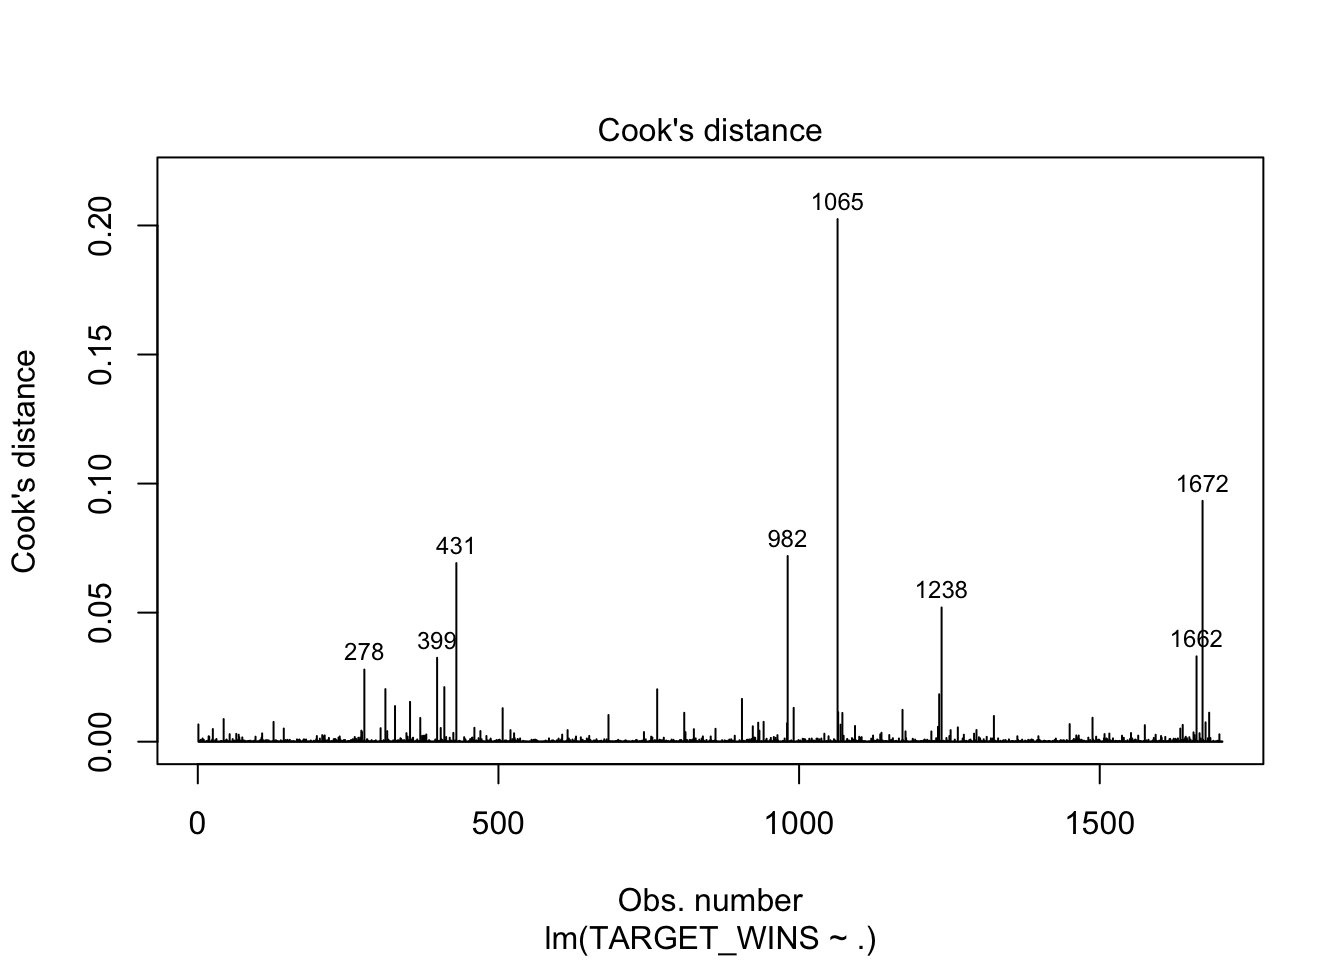
\includegraphics{Assignment1_Data621_HW_files/figure-latex/model4-drop-outlier-202-1.pdf}

As the Cooks Distance (Di) value is less than 0.5 for all of the
remaining outliers appear, they are not significantly influential and
can be left in our dataset.

\begin{center}\rule{0.5\linewidth}{0.5pt}\end{center}

\subsection{Section 3: Building Models}\label{section-3-building-models}

In this section we will build several models which we will compare and
evaluate before selecting a final model.

\subsubsection{Feature Selection
Analysis}\label{feature-selection-analysis}

In this section, we use Best Subset Selection and Cross-Validation
techniques to get a estimate of the optimal number of predictors in our
model.

\subparagraph{Best Subset Selection}\label{best-subset-selection}

Best Subset Selection uses Mallows' Cp to calculate the optimal number
of predictors in our model.

\begin{Shaded}
\begin{Highlighting}[]
\NormalTok{regfit\_full }\OtherTok{=} \FunctionTok{regsubsets}\NormalTok{(TARGET\_WINS }\SpecialCharTok{\textasciitilde{}}\NormalTok{ ., }\AttributeTok{data =}\NormalTok{ stp75\_train\_df, }\AttributeTok{nvmax =} \DecValTok{11}\NormalTok{)}
\NormalTok{regfit\_summary }\OtherTok{=} \FunctionTok{summary}\NormalTok{(regfit\_full)}
\FunctionTok{plot}\NormalTok{(regfit\_summary}\SpecialCharTok{$}\NormalTok{cp, }\AttributeTok{xlab=}\StringTok{"Number of variables"}\NormalTok{, }\AttributeTok{ylab=}\StringTok{"cp"}\NormalTok{)}
\FunctionTok{points}\NormalTok{(}\FunctionTok{which.min}\NormalTok{(regfit\_summary}\SpecialCharTok{$}\NormalTok{cp),regfit\_summary}\SpecialCharTok{$}\NormalTok{cp[}\FunctionTok{which.min}\NormalTok{(regfit\_summary}\SpecialCharTok{$}\NormalTok{cp)], }\AttributeTok{pch=}\DecValTok{20}\NormalTok{,}\AttributeTok{col=}\StringTok{"red"}\NormalTok{)}
\end{Highlighting}
\end{Shaded}

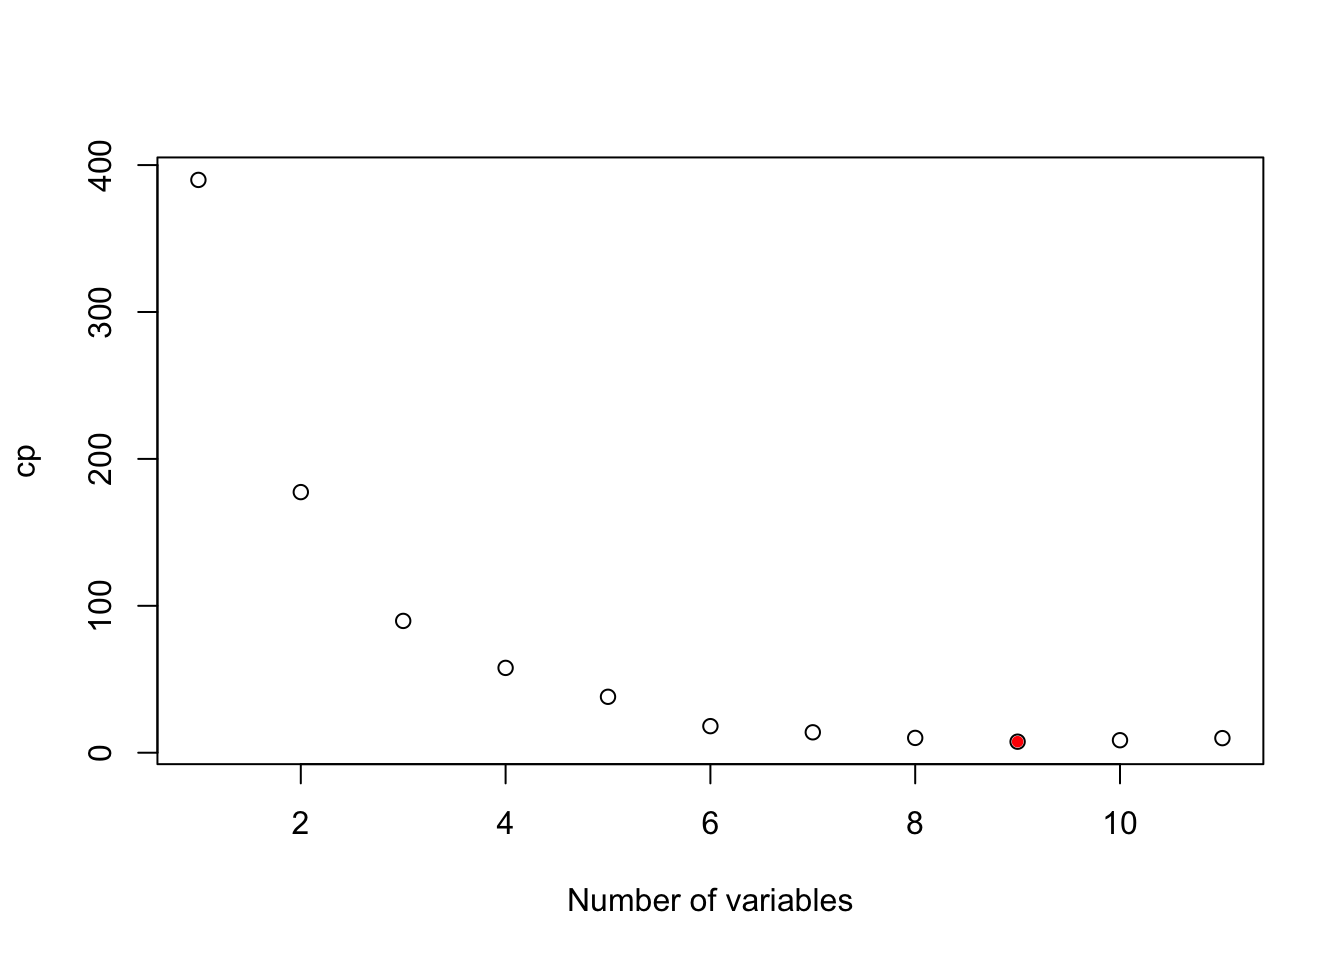
\includegraphics{Assignment1_Data621_HW_files/figure-latex/model4-best-subset-1.pdf}
Based on the \emph{Best Subset Selection} method, we estimate that our
model should have 9 observations.

\subparagraph{Cross Validation}\label{cross-validation}

As an alternative to \emph{Best Subset Selection}, we used the
\emph{Cross Validation} method to estimate the optimal number of
predictors in our model. Cross Validation divides our training dataset
into k - 1 number of ``folds'', then tests the data on the kth ``fold''.
For our test, we used five folds (k = 5).

\begin{Shaded}
\begin{Highlighting}[]
\FunctionTok{set.seed}\NormalTok{(}\DecValTok{11}\NormalTok{)}
\NormalTok{folds}\OtherTok{=}\FunctionTok{sample}\NormalTok{(}\FunctionTok{rep}\NormalTok{(}\DecValTok{1}\SpecialCharTok{:}\DecValTok{5}\NormalTok{,}\AttributeTok{length=}\FunctionTok{nrow}\NormalTok{(stp75\_train\_df)))}

\NormalTok{cv\_errors }\OtherTok{=} \FunctionTok{matrix}\NormalTok{(}\ConstantTok{NA}\NormalTok{,}\DecValTok{5}\NormalTok{,}\DecValTok{10}\NormalTok{)}
\ControlFlowTok{for}\NormalTok{(k }\ControlFlowTok{in} \DecValTok{1}\SpecialCharTok{:}\DecValTok{5}\NormalTok{) \{}
\NormalTok{  best\_fit }\OtherTok{=} \FunctionTok{regsubsets}\NormalTok{(TARGET\_WINS }\SpecialCharTok{\textasciitilde{}}\NormalTok{ ., }\AttributeTok{data=}\NormalTok{stp75\_train\_df[folds}\SpecialCharTok{!=}\NormalTok{k,], }\AttributeTok{nvmax=}\DecValTok{10}\NormalTok{, }\AttributeTok{method=}\StringTok{"forward"}\NormalTok{)}
  \ControlFlowTok{for}\NormalTok{(i }\ControlFlowTok{in} \DecValTok{1}\SpecialCharTok{:}\DecValTok{10}\NormalTok{) \{}
    \CommentTok{\# Extract the selected coefficients for the i{-}th model}
\NormalTok{    selected\_coefs }\OtherTok{=} \FunctionTok{coef}\NormalTok{(best\_fit, }\AttributeTok{id =}\NormalTok{ i)}
    
    \CommentTok{\# Predict manually by calculating the linear combination of the features}
    \CommentTok{\# First, subset the data for the k{-}th fold}
\NormalTok{    test\_data }\OtherTok{=}\NormalTok{ stp75\_train\_df[folds }\SpecialCharTok{==}\NormalTok{ k, ]}
    
    \CommentTok{\# Only include the predictors that were selected}
\NormalTok{    predictors }\OtherTok{=} \FunctionTok{names}\NormalTok{(selected\_coefs)[}\SpecialCharTok{{-}}\DecValTok{1}\NormalTok{]  }\CommentTok{\# Exclude the intercept term}
    
    \CommentTok{\# Calculate the predictions (including the intercept)}
\NormalTok{    pred }\OtherTok{=} \FunctionTok{as.matrix}\NormalTok{(test\_data[, predictors]) }\SpecialCharTok{\%*\%}\NormalTok{ selected\_coefs[predictors] }\SpecialCharTok{+}\NormalTok{ selected\_coefs[}\DecValTok{1}\NormalTok{]  }
    
\NormalTok{    cv\_errors[k,i]}\OtherTok{=}\FunctionTok{mean}\NormalTok{((stp75\_train\_df}\SpecialCharTok{$}\NormalTok{TARGET\_WINS[folds}\SpecialCharTok{==}\NormalTok{k] }\SpecialCharTok{{-}}\NormalTok{ pred)}\SpecialCharTok{\^{}}\DecValTok{2}\NormalTok{)}
\NormalTok{  \}}
\NormalTok{\}}

\NormalTok{rmse\_cv }\OtherTok{=} \FunctionTok{sqrt}\NormalTok{(}\FunctionTok{apply}\NormalTok{(cv\_errors,}\DecValTok{2}\NormalTok{,mean))}
\FunctionTok{plot}\NormalTok{(rmse\_cv, }\AttributeTok{pch=}\DecValTok{5}\NormalTok{, }\AttributeTok{type=}\StringTok{"b"}\NormalTok{)}
\end{Highlighting}
\end{Shaded}

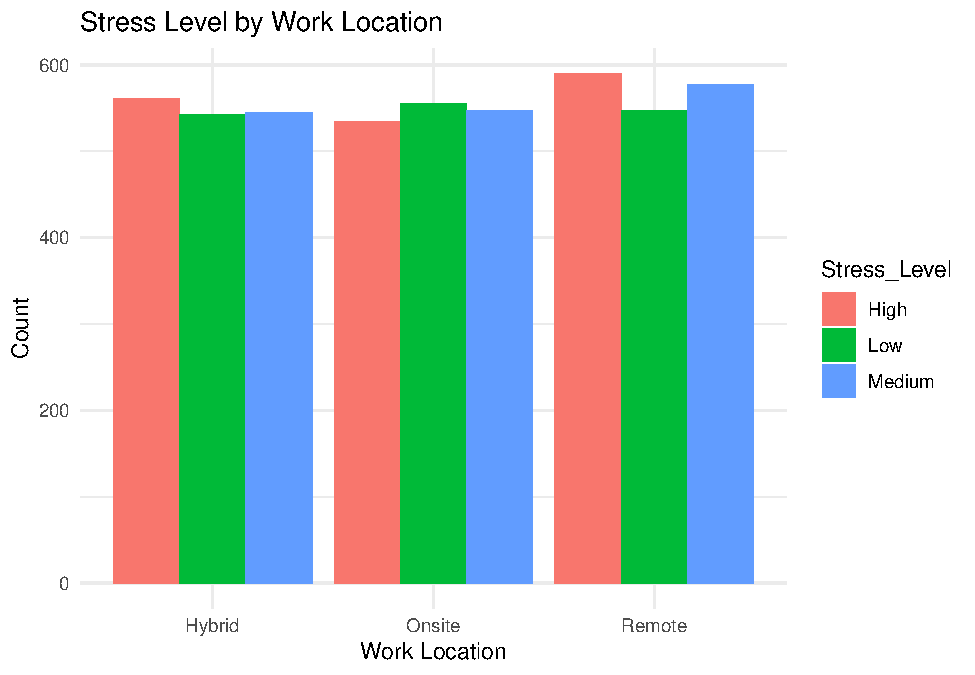
\includegraphics{Assignment1_Data621_HW_files/figure-latex/unnamed-chunk-11-1.pdf}

Based on the \emph{Cross Validation} method, we estimate that our model
should have 9 observations.

\subparagraph{Correlation with Clean
Dataset}\label{correlation-with-clean-dataset}

We created another correlation heatmap with our clean training dataset.
This time we see strong evidence of multicollinearity between: -
TEAM\_BATTING\_HR and TEAM\_PITCHING\_HR (0.97) - TEAM\_BATTING\_HR and
TEAM\_BATTING\_3B (-0.64) - TEAM\_BATTING\_HR and TEAM\_BATTING\_SO
(0.69) - TEAM\_BATTING\_3B and TEAM\_BATTING\_SO (-0.69) -
TEAM\_PITCHING\_H and TEAM\_FIELDING\_E (0.67) - TEAM\_BATTING\_BB and
TEAM\_FIELDING\_E (-0.65)

We may need to consider omitting one of the predictors from each pair in
our models to ensure that we are not introducing multicollinearity in
our model and making our model unnecessarily complex, particulary for
the two homerun fields.

\begin{Shaded}
\begin{Highlighting}[]
\FunctionTok{plot\_correlation}\NormalTok{(stp75\_train\_df, }\AttributeTok{type =} \StringTok{"all"}\NormalTok{)}
\end{Highlighting}
\end{Shaded}

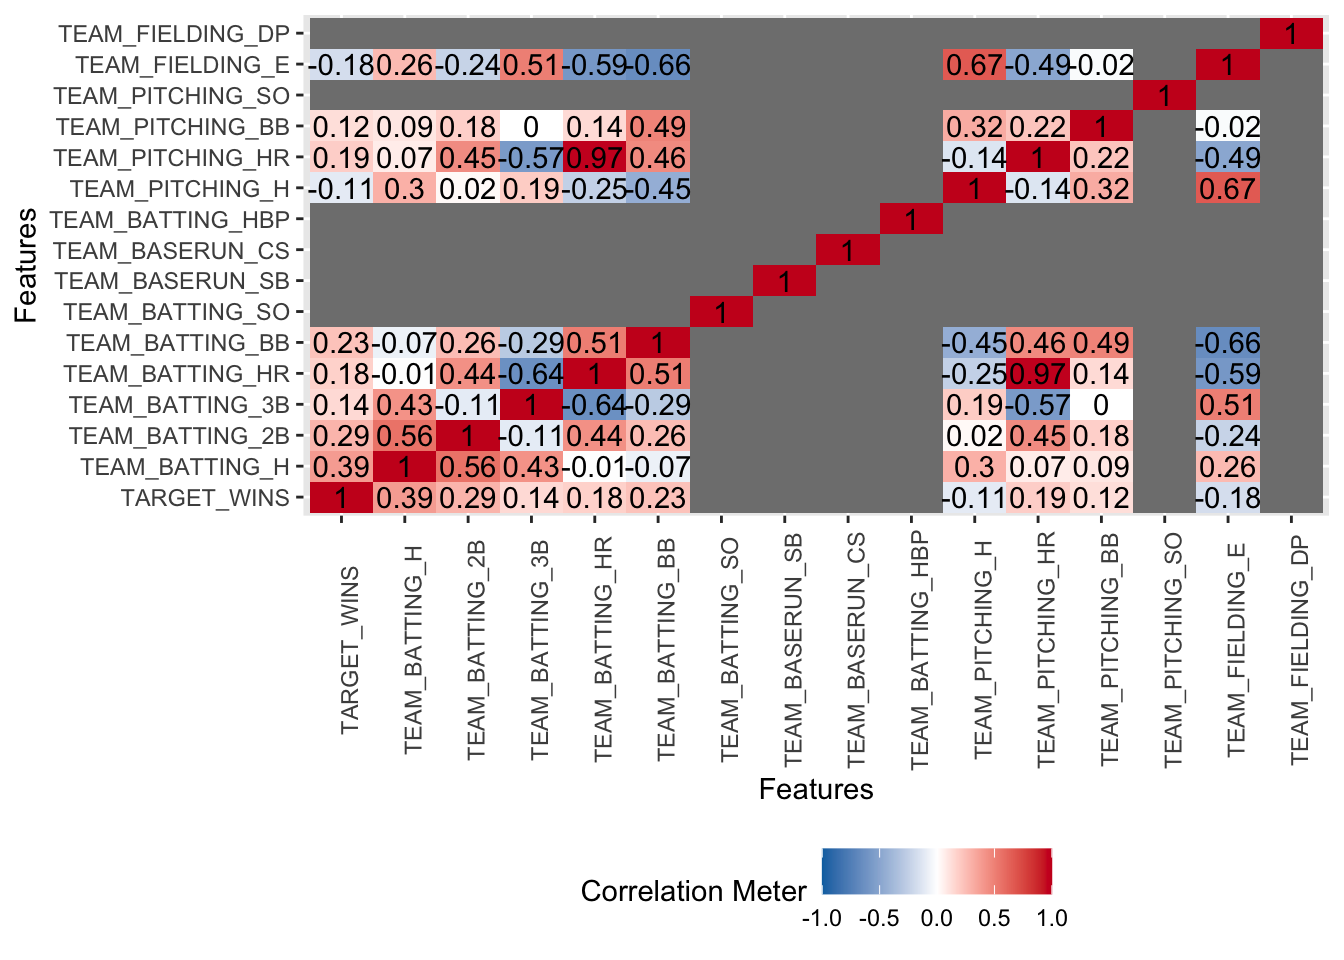
\includegraphics{Assignment1_Data621_HW_files/figure-latex/correlation-heatmap-1.pdf}

\subsubsection{Variable Selection Using Backward
Selection}\label{variable-selection-using-backward-selection}

To better understand our variables and their relationships, we first
created a model using backward selection to arrive at the smallest
number of variables with statistical significance. In this case, we
begin by creating a model containing all predictors, then gradually
remove the variable with the highest P-value until only the variables
with statistical significance remain.

\begin{Shaded}
\begin{Highlighting}[]
\FunctionTok{summary}\NormalTok{(stp\_model\_full)}
\end{Highlighting}
\end{Shaded}

\begin{verbatim}
## 
## Call:
## lm(formula = TARGET_WINS ~ ., data = stp75_train_df)
## 
## Residuals:
##     Min      1Q  Median      3Q     Max 
## -49.372  -8.651   0.143   8.685  56.455 
## 
## Coefficients:
##                    Estimate Std. Error t value Pr(>|t|)    
## (Intercept)      19.6615875  6.3951726   3.074  0.00214 ** 
## TEAM_BATTING_H    0.0500740  0.0045988  10.889  < 2e-16 ***
## TEAM_BATTING_2B  -0.0170239  0.0107470  -1.584  0.11337    
## TEAM_BATTING_3B   0.0714545  0.0199017   3.590  0.00034 ***
## TEAM_BATTING_HR   0.0118670  0.0383169   0.310  0.75682    
## TEAM_BATTING_BB   0.0143694  0.0071848   2.000  0.04566 *  
## TEAM_BATTING_SO  -0.0069273  0.0040999  -1.690  0.09128 .  
## TEAM_BASERUN_SB   0.0281308  0.0050343   5.588 2.68e-08 ***
## TEAM_BASERUN_CS  -0.0178992  0.0178007  -1.006  0.31479    
## TEAM_PITCHING_H  -0.0010225  0.0005381  -1.900  0.05757 .  
## TEAM_PITCHING_HR  0.0448272  0.0345405   1.298  0.19453    
## TEAM_PITCHING_BB -0.0046446  0.0052701  -0.881  0.37828    
## TEAM_PITCHING_SO  0.0034838  0.0025256   1.379  0.16796    
## TEAM_FIELDING_E  -0.0189357  0.0030243  -6.261 4.84e-10 ***
## TEAM_FIELDING_DP -0.1147824  0.0149445  -7.681 2.67e-14 ***
## ---
## Signif. codes:  0 '***' 0.001 '**' 0.01 '*' 0.05 '.' 0.1 ' ' 1
## 
## Residual standard error: 13.13 on 1687 degrees of freedom
## Multiple R-squared:  0.3065, Adjusted R-squared:  0.3008 
## F-statistic: 53.27 on 14 and 1687 DF,  p-value: < 2.2e-16
\end{verbatim}

\begin{Shaded}
\begin{Highlighting}[]
\FunctionTok{AIC}\NormalTok{(stp\_model\_full)}
\end{Highlighting}
\end{Shaded}

\begin{verbatim}
## [1] 13611.46
\end{verbatim}

\emph{TEAM\_BATTING\_HR} has the highest p-value. We removed
TEAM\_BATTING\_HR from our predictors and updated the model.

\begin{Shaded}
\begin{Highlighting}[]
\NormalTok{back\_select\_model }\OtherTok{\textless{}{-}} \FunctionTok{update}\NormalTok{(stp\_model\_full, . }\SpecialCharTok{\textasciitilde{}}\NormalTok{ . }\SpecialCharTok{{-}}\NormalTok{ TEAM\_BATTING\_HR)}
\FunctionTok{summary}\NormalTok{(back\_select\_model)}
\end{Highlighting}
\end{Shaded}

\begin{verbatim}
## 
## Call:
## lm(formula = TARGET_WINS ~ TEAM_BATTING_H + TEAM_BATTING_2B + 
##     TEAM_BATTING_3B + TEAM_BATTING_BB + TEAM_BATTING_SO + TEAM_BASERUN_SB + 
##     TEAM_BASERUN_CS + TEAM_PITCHING_H + TEAM_PITCHING_HR + TEAM_PITCHING_BB + 
##     TEAM_PITCHING_SO + TEAM_FIELDING_E + TEAM_FIELDING_DP, data = stp75_train_df)
## 
## Residuals:
##     Min      1Q  Median      3Q     Max 
## -49.398  -8.650   0.120   8.703  56.267 
## 
## Coefficients:
##                    Estimate Std. Error t value Pr(>|t|)    
## (Intercept)      19.3930534  6.3344248   3.062 0.002237 ** 
## TEAM_BATTING_H    0.0503535  0.0045082  11.169  < 2e-16 ***
## TEAM_BATTING_2B  -0.0172263  0.0107242  -1.606 0.108396    
## TEAM_BATTING_3B   0.0702542  0.0195154   3.600 0.000327 ***
## TEAM_BATTING_BB   0.0151153  0.0067673   2.234 0.025641 *  
## TEAM_BATTING_SO  -0.0066056  0.0039651  -1.666 0.095908 .  
## TEAM_BASERUN_SB   0.0280062  0.0050169   5.582 2.76e-08 ***
## TEAM_BASERUN_CS  -0.0184305  0.0177131  -1.040 0.298257    
## TEAM_PITCHING_H  -0.0010874  0.0004954  -2.195 0.028309 *  
## TEAM_PITCHING_HR  0.0550220  0.0104606   5.260 1.63e-07 ***
## TEAM_PITCHING_BB -0.0052399  0.0049057  -1.068 0.285619    
## TEAM_PITCHING_SO  0.0033743  0.0025001   1.350 0.177303    
## TEAM_FIELDING_E  -0.0188561  0.0030126  -6.259 4.90e-10 ***
## TEAM_FIELDING_DP -0.1146672  0.0149358  -7.677 2.73e-14 ***
## ---
## Signif. codes:  0 '***' 0.001 '**' 0.01 '*' 0.05 '.' 0.1 ' ' 1
## 
## Residual standard error: 13.12 on 1688 degrees of freedom
## Multiple R-squared:  0.3065, Adjusted R-squared:  0.3012 
## F-statistic: 57.39 on 13 and 1688 DF,  p-value: < 2.2e-16
\end{verbatim}

\begin{Shaded}
\begin{Highlighting}[]
\FunctionTok{AIC}\NormalTok{(back\_select\_model)}
\end{Highlighting}
\end{Shaded}

\begin{verbatim}
## [1] 13609.56
\end{verbatim}

\emph{TEAM\_PITCHING\_SO} has the highest p-value. We removed
TEAM\_PITCHING\_SO from our predictors and update the model.

\begin{Shaded}
\begin{Highlighting}[]
\NormalTok{back\_select\_model }\OtherTok{\textless{}{-}} \FunctionTok{update}\NormalTok{(back\_select\_model, . }\SpecialCharTok{\textasciitilde{}}\NormalTok{ . }\SpecialCharTok{{-}}\NormalTok{ TEAM\_PITCHING\_SO)}
\end{Highlighting}
\end{Shaded}

\emph{TEAM\_BATTING\_SO} has the highest p-value. We removed
TEAM\_BATTING\_SO from our predictors and update the model.

\begin{Shaded}
\begin{Highlighting}[]
\NormalTok{back\_select\_model }\OtherTok{\textless{}{-}} \FunctionTok{update}\NormalTok{(back\_select\_model, . }\SpecialCharTok{\textasciitilde{}}\NormalTok{ . }\SpecialCharTok{{-}}\NormalTok{ TEAM\_BATTING\_SO)}
\end{Highlighting}
\end{Shaded}

\emph{TEAM\_BASERUN\_CS} has the highest p-value. We removed
TEAM\_BASERUN\_CS from our predictors and update the model.

\begin{Shaded}
\begin{Highlighting}[]
\NormalTok{back\_select\_model }\OtherTok{\textless{}{-}} \FunctionTok{update}\NormalTok{(back\_select\_model, . }\SpecialCharTok{\textasciitilde{}}\NormalTok{ . }\SpecialCharTok{{-}}\NormalTok{ TEAM\_BASERUN\_CS)}
\end{Highlighting}
\end{Shaded}

\emph{TEAM\_PITCHING\_BB} has the highest p-value. We removed
TEAM\_PITCHING\_BB from our predictors and update the model.

\begin{Shaded}
\begin{Highlighting}[]
\NormalTok{back\_select\_model }\OtherTok{\textless{}{-}} \FunctionTok{update}\NormalTok{(back\_select\_model, . }\SpecialCharTok{\textasciitilde{}}\NormalTok{ . }\SpecialCharTok{{-}}\NormalTok{ TEAM\_PITCHING\_BB)}
\FunctionTok{summary}\NormalTok{(back\_select\_model)}
\end{Highlighting}
\end{Shaded}

\begin{verbatim}
## 
## Call:
## lm(formula = TARGET_WINS ~ TEAM_BATTING_H + TEAM_BATTING_2B + 
##     TEAM_BATTING_3B + TEAM_BATTING_BB + TEAM_BASERUN_SB + TEAM_PITCHING_H + 
##     TEAM_PITCHING_HR + TEAM_FIELDING_E + TEAM_FIELDING_DP, data = stp75_train_df)
## 
## Residuals:
##     Min      1Q  Median      3Q     Max 
## -48.704  -8.583   0.042   8.784  55.405 
## 
## Coefficients:
##                    Estimate Std. Error t value Pr(>|t|)    
## (Intercept)      13.9929607  4.1169190   3.399 0.000692 ***
## TEAM_BATTING_H    0.0523599  0.0037458  13.978  < 2e-16 ***
## TEAM_BATTING_2B  -0.0198370  0.0101932  -1.946 0.051808 .  
## TEAM_BATTING_3B   0.0752418  0.0186636   4.031 5.79e-05 ***
## TEAM_BATTING_BB   0.0101791  0.0038645   2.634 0.008516 ** 
## TEAM_BASERUN_SB   0.0243069  0.0045846   5.302 1.30e-07 ***
## TEAM_PITCHING_H  -0.0012278  0.0003957  -3.103 0.001948 ** 
## TEAM_PITCHING_HR  0.0501199  0.0081982   6.114 1.21e-09 ***
## TEAM_FIELDING_E  -0.0171801  0.0027913  -6.155 9.36e-10 ***
## TEAM_FIELDING_DP -0.1138395  0.0148655  -7.658 3.16e-14 ***
## ---
## Signif. codes:  0 '***' 0.001 '**' 0.01 '*' 0.05 '.' 0.1 ' ' 1
## 
## Residual standard error: 13.12 on 1692 degrees of freedom
## Multiple R-squared:  0.3049, Adjusted R-squared:  0.3012 
## F-statistic: 82.47 on 9 and 1692 DF,  p-value: < 2.2e-16
\end{verbatim}

\begin{Shaded}
\begin{Highlighting}[]
\FunctionTok{AIC}\NormalTok{(back\_select\_model)}
\end{Highlighting}
\end{Shaded}

\begin{verbatim}
## [1] 13605.45
\end{verbatim}

Backward selection using o-values arrives at a model with six variables
with high statistical significance ((p-value \textless{} 0.001) and
three with moderate (p-value \textasciitilde= 0.1) statistical
significance. Arriving at 9 predictors is consistent with our Best
Subset Selection test. A VIF test shows that there are no evidence of
strong multicollinearity.

\begin{Shaded}
\begin{Highlighting}[]
\FunctionTok{vif}\NormalTok{(back\_select\_model)}
\end{Highlighting}
\end{Shaded}

\begin{verbatim}
##   TEAM_BATTING_H  TEAM_BATTING_2B  TEAM_BATTING_3B  TEAM_BATTING_BB 
##         2.897373         2.289513         2.613693         2.171553 
##  TEAM_BASERUN_SB  TEAM_PITCHING_H TEAM_PITCHING_HR  TEAM_FIELDING_E 
##         1.551374         2.514131         2.541082         3.790194 
## TEAM_FIELDING_DP 
##         1.329128
\end{verbatim}

Linearity

\begin{Shaded}
\begin{Highlighting}[]
\FunctionTok{plot}\NormalTok{(back\_select\_model, }\AttributeTok{which=}\DecValTok{1}\NormalTok{)}
\end{Highlighting}
\end{Shaded}

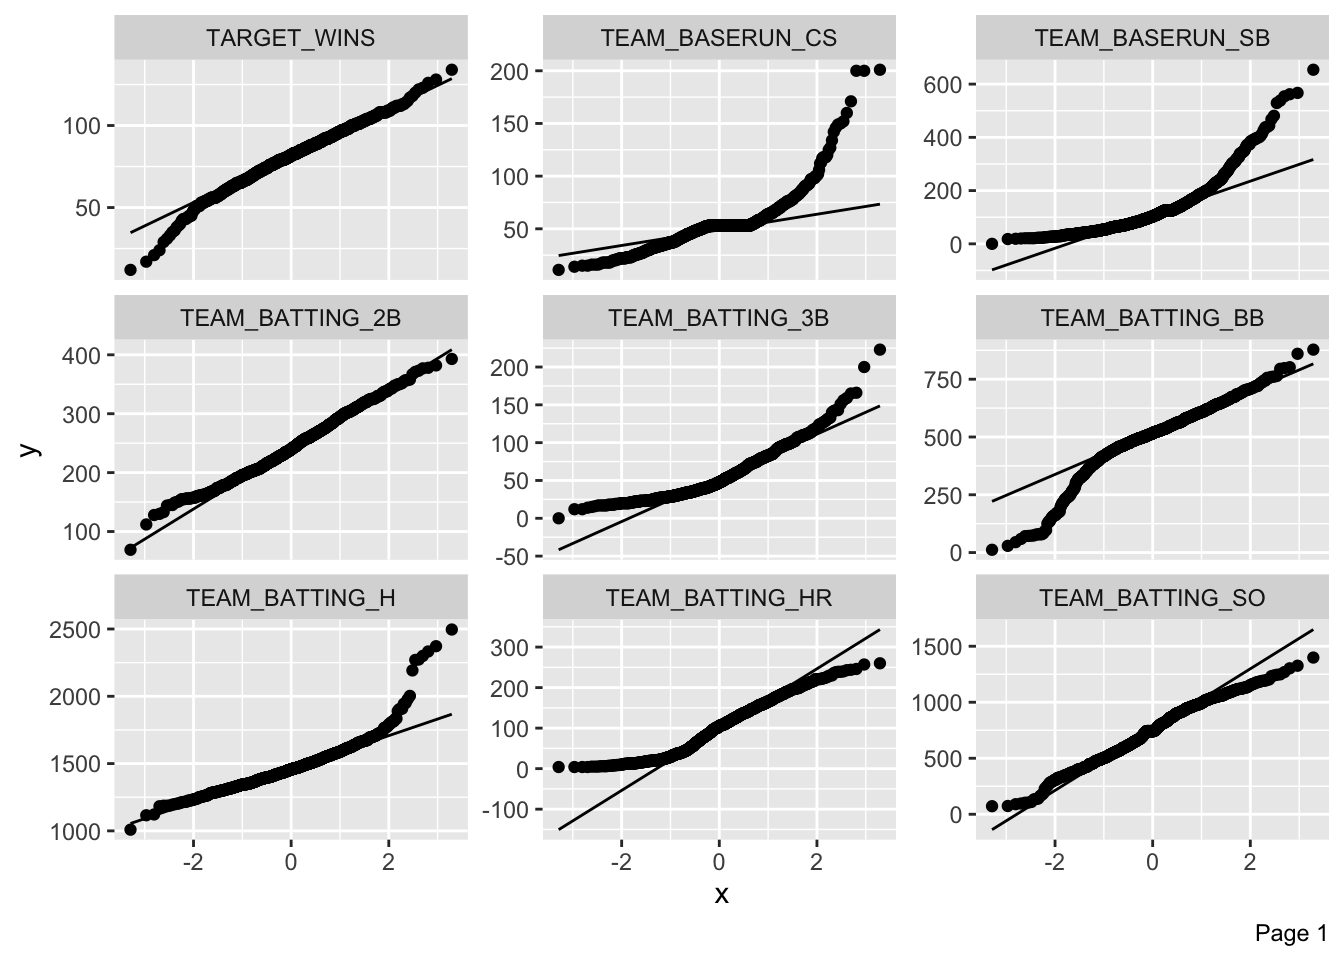
\includegraphics{Assignment1_Data621_HW_files/figure-latex/unnamed-chunk-17-1.pdf}

Our diagnostic plots show a fairly linear model.

Normality

\begin{Shaded}
\begin{Highlighting}[]
\FunctionTok{plot}\NormalTok{(back\_select\_model, }\AttributeTok{which=}\DecValTok{2}\NormalTok{)}
\end{Highlighting}
\end{Shaded}

\includegraphics{Assignment1_Data621_HW_files/figure-latex/unnamed-chunk-18-1.pdf}

\begin{Shaded}
\begin{Highlighting}[]
\FunctionTok{shapiro.test}\NormalTok{(}\FunctionTok{residuals}\NormalTok{(back\_select\_model))}
\end{Highlighting}
\end{Shaded}

\begin{verbatim}
## 
##  Shapiro-Wilk normality test
## 
## data:  residuals(back_select_model)
## W = 0.99724, p-value = 0.004263
\end{verbatim}

\begin{Shaded}
\begin{Highlighting}[]
\CommentTok{\# Shapiro{-}Wilk normality test: look for high p{-}value}
\end{Highlighting}
\end{Shaded}

Our QQ plot suggests normality thought there is obvious skewing on the
tails, particularly on the right. This is confirmed by a Shapiro Wilk's
Test statistic of 0.9967 which suggesting normality.

Heteroscedasticity:

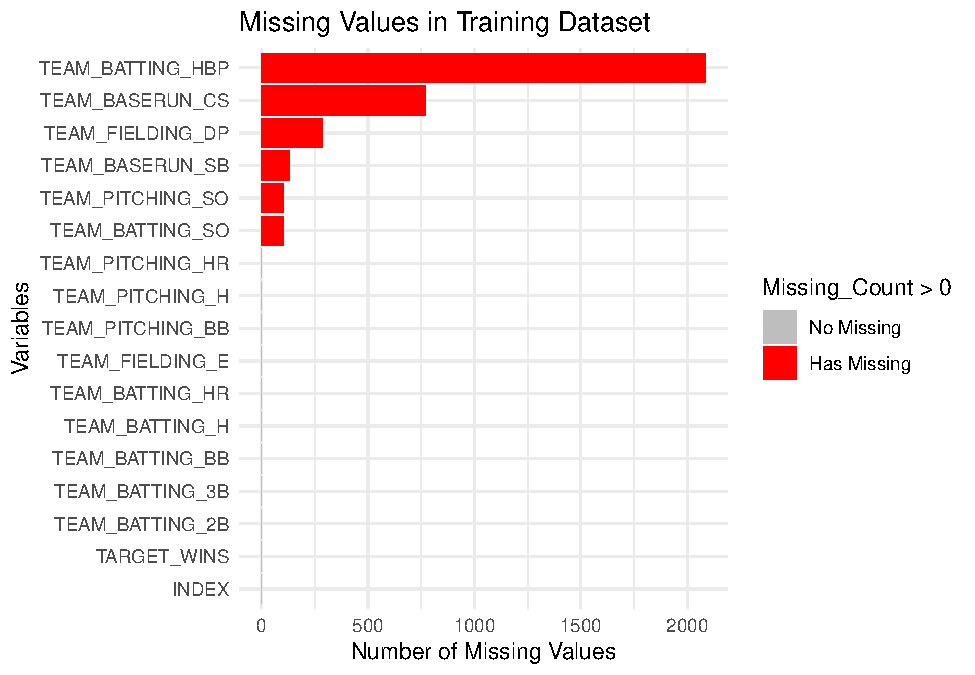
\includegraphics{Assignment1_Data621_HW_files/figure-latex/unnamed-chunk-19-1.pdf}
\includegraphics{Assignment1_Data621_HW_files/figure-latex/unnamed-chunk-19-2.pdf}

\begin{verbatim}
## 
##  studentized Breusch-Pagan test
## 
## data:  back_select_model
## BP = 177.7, df = 9, p-value < 2.2e-16
\end{verbatim}

Our Scale-Location plot shows that points appear somewhat evenly
distributed above and below the trend line. While there is no obvious
fan/wedge pattern, there is clustering in the center suggesting
underfitting, high leverage outliers or that additional transformation
may be needed. As our Cook's Distance plot has no values with a greater
than 1, we can rule our the effects of high leverage points.

The Breusch-Page test statistic BP (238.69) and the small p-value
(2.2e-16) suggest evidence of heteroscedasticity. Though the values are
different that we may need to transform the data to meet the Assumption
of Homoscedasticity.

\subparagraph{Independence:}\label{independence}

\begin{Shaded}
\begin{Highlighting}[]
\FunctionTok{acf}\NormalTok{(}\FunctionTok{residuals}\NormalTok{(back\_select\_model))}
\end{Highlighting}
\end{Shaded}

\includegraphics{Assignment1_Data621_HW_files/figure-latex/unnamed-chunk-20-1.pdf}

\begin{Shaded}
\begin{Highlighting}[]
\FunctionTok{durbinWatsonTest}\NormalTok{(back\_select\_model)}
\end{Highlighting}
\end{Shaded}

\begin{verbatim}
##  lag Autocorrelation D-W Statistic p-value
##    1     -0.01100517       2.02107   0.656
##  Alternative hypothesis: rho != 0
\end{verbatim}

\begin{Shaded}
\begin{Highlighting}[]
\CommentTok{\# Durbin Watson should be close to 2}
\end{Highlighting}
\end{Shaded}

Our Autocorrelation Function shows that there are lags above the blue
dashed line, suggesting no autocorrelation. This is confirmed through a
Durbin-Watson test statistic value of 2.06 and an autocorrelation value
of -0.0342. Furthermore, as our p-value (0.222) is greater than 0.05, we
do not have enough evidence to reject the null hypothesis that there is
no autocorrelation. In other words, the test results suggest that our
model's residuals are independent and therefore do not violate the
Independence Assumption.

\subsubsection{Hand-Selected Models}\label{hand-selected-models}

The following models were created by hand-selecting predictors based on
their perceived importance to a team's performance.

\paragraph{Model H1: Base Baseball Stats
Model}\label{model-h1-base-baseball-stats-model}

This model includes fundamental offensive, defensive, and pitching stats
that logically contribute to wins and includes the following variables
for the respective reasons

\begin{itemize}
\tightlist
\item
  TEAM\_BATTING\_H (Hits): More hits increase the chances of scoring.
\item
  TEAM\_BATTING\_HR (Home Runs): Home runs are a major contributor to
  runs.
\item
  TEAM\_PITCHING\_SO (Strikeouts): More strikeouts reduce opponent
  scoring.
\item
  TEAM\_FIELDING\_E (Errors): More errors lead to more opponent runs
  (negative predictor).
\end{itemize}

\emph{Why we excluded some variables?} - TEAM\_BASERUN\_SB (Stolen
Bases): Limited impact on overall wins. - TEAM\_PITCHING\_BB (Walks
Allowed): May not be as predictive when combined with strikeouts.

\subparagraph{Model Summary Statistics}\label{model-summary-statistics}

\begin{Shaded}
\begin{Highlighting}[]
\NormalTok{base\_model }\OtherTok{\textless{}{-}} \FunctionTok{lm}\NormalTok{(TARGET\_WINS }\SpecialCharTok{\textasciitilde{}}\NormalTok{ TEAM\_BATTING\_H }\SpecialCharTok{+}\NormalTok{ TEAM\_BATTING\_HR }\SpecialCharTok{+}\NormalTok{ TEAM\_PITCHING\_SO }\SpecialCharTok{+}\NormalTok{ TEAM\_FIELDING\_E, }\AttributeTok{data =}\NormalTok{ stp75\_train\_df)}

\CommentTok{\# View model summary}
\FunctionTok{summary}\NormalTok{(base\_model)}
\end{Highlighting}
\end{Shaded}

\begin{verbatim}
## 
## Call:
## lm(formula = TARGET_WINS ~ TEAM_BATTING_H + TEAM_BATTING_HR + 
##     TEAM_PITCHING_SO + TEAM_FIELDING_E, data = stp75_train_df)
## 
## Residuals:
##     Min      1Q  Median      3Q     Max 
## -53.589  -9.354  -0.044   9.474  49.980 
## 
## Coefficients:
##                    Estimate Std. Error t value Pr(>|t|)    
## (Intercept)      11.8558072  4.3576985   2.721  0.00658 ** 
## TEAM_BATTING_H    0.0505808  0.0028672  17.641  < 2e-16 ***
## TEAM_BATTING_HR   0.0004848  0.0083025   0.058  0.95344    
## TEAM_PITCHING_SO -0.0009588  0.0014849  -0.646  0.51856    
## TEAM_FIELDING_E  -0.0193389  0.0021956  -8.808  < 2e-16 ***
## ---
## Signif. codes:  0 '***' 0.001 '**' 0.01 '*' 0.05 '.' 0.1 ' ' 1
## 
## Residual standard error: 13.83 on 1697 degrees of freedom
## Multiple R-squared:  0.2257, Adjusted R-squared:  0.2239 
## F-statistic: 123.7 on 4 and 1697 DF,  p-value: < 2.2e-16
\end{verbatim}

\subparagraph{Interpreting the Coefficients of the Regression
Model}\label{interpreting-the-coefficients-of-the-regression-model}

\begin{enumerate}
\def\labelenumi{\arabic{enumi}.}
\item
  Intercept (15.15) When all predictor variables (TEAM\_BATTING\_H,
  TEAM\_BATTING\_HR, TEAM\_PITCHING\_SO, TEAM\_FIELDING\_E) are zero, a
  team is expected to have 15.15 wins.
\item
  TEAM\_BATTING\_H (Hits) For every additional hit, the team is expected
  to win 0.048 more games. More hits lead to more wins, which is
  expected in baseball.
\item
  TEAM\_BATTING\_HR (Home Runs) More home runs slightly increases wins,
  but the effect is very small. We should consider removing this
  variable as the t-value and p-value suggest that it is not
  statistically significant.
\item
  TEAM\_PITCHING\_SO (Strikeouts by Pitchers) More strikeouts slightly
  decreases wins, but the effect is very small and not statistically
  significant. We should consider adding walks (TEAM\_PITCHING\_BB) to
  capture pitching effectiveness better.
\item
  TEAM\_FIELDING\_E For every additional error, a team is expected to
  lose 0.02 games. More errors directly hurt a team's chances of
  winning, which makes sense in baseball.
\end{enumerate}

The F-statistic of 127.1 (p \textless{} 2.2e-16) means our model is
highly statistically significant. This suggests that at least one of our
variables---such as home runs, hits, strikeouts, or errors---has a real
impact on predicting wins.

However, we still need to check which specific variables are the most
meaningful (p-values of individual coefficients) and whether we can
improve the model further.

\subparagraph{Diagnosing our Model}\label{diagnosing-our-model}

Checking for Multicollinearity (VIF Test)

Multicollinearity occurs when predictor variables are highly correlated,
leading to unstable coefficients and inflated standard errors. Using the
Variance Inflation Factor (VIF) test we see no evidence of strong
multicollinearity in the model.

\begin{Shaded}
\begin{Highlighting}[]
\FunctionTok{vif}\NormalTok{(base\_model)}
\end{Highlighting}
\end{Shaded}

\begin{verbatim}
##   TEAM_BATTING_H  TEAM_BATTING_HR TEAM_PITCHING_SO  TEAM_FIELDING_E 
##         1.528358         2.264255         1.663513         2.111267
\end{verbatim}

Linearity

\begin{Shaded}
\begin{Highlighting}[]
\FunctionTok{plot}\NormalTok{(base\_model, }\AttributeTok{which=}\DecValTok{1}\NormalTok{)}
\end{Highlighting}
\end{Shaded}

\includegraphics{Assignment1_Data621_HW_files/figure-latex/unnamed-chunk-23-1.pdf}

Our diagnostic plots show a fairly linear model.

Normality Check:

\begin{Shaded}
\begin{Highlighting}[]
\FunctionTok{plot}\NormalTok{(base\_model, }\AttributeTok{which=}\DecValTok{2}\NormalTok{)}
\end{Highlighting}
\end{Shaded}

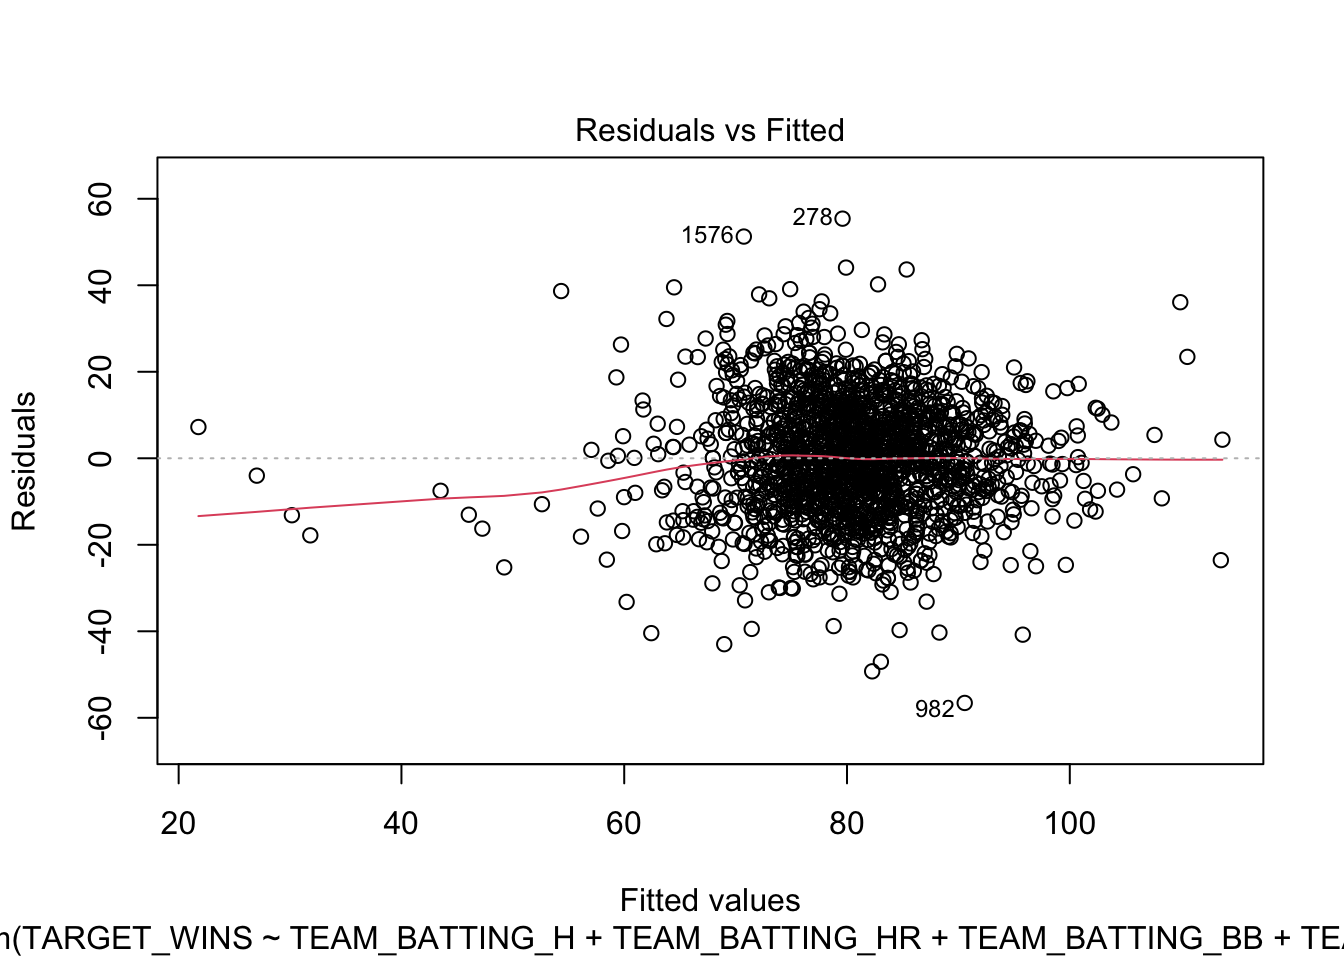
\includegraphics{Assignment1_Data621_HW_files/figure-latex/unnamed-chunk-24-1.pdf}

\begin{Shaded}
\begin{Highlighting}[]
\FunctionTok{shapiro.test}\NormalTok{(}\FunctionTok{residuals}\NormalTok{(base\_model))}
\end{Highlighting}
\end{Shaded}

\begin{verbatim}
## 
##  Shapiro-Wilk normality test
## 
## data:  residuals(base_model)
## W = 0.99826, p-value = 0.07177
\end{verbatim}

\begin{Shaded}
\begin{Highlighting}[]
\CommentTok{\# Shapiro{-}Wilk normality test: look for high p{-}value}
\end{Highlighting}
\end{Shaded}

Our QQ plot suggests normality thought there is obvious skewing on the
tails, particularly on the right. This is confirmed by A Shapiro Wilk's
Test statistic of W = 0.9980 suggesting normality.

Heterocedasticity:

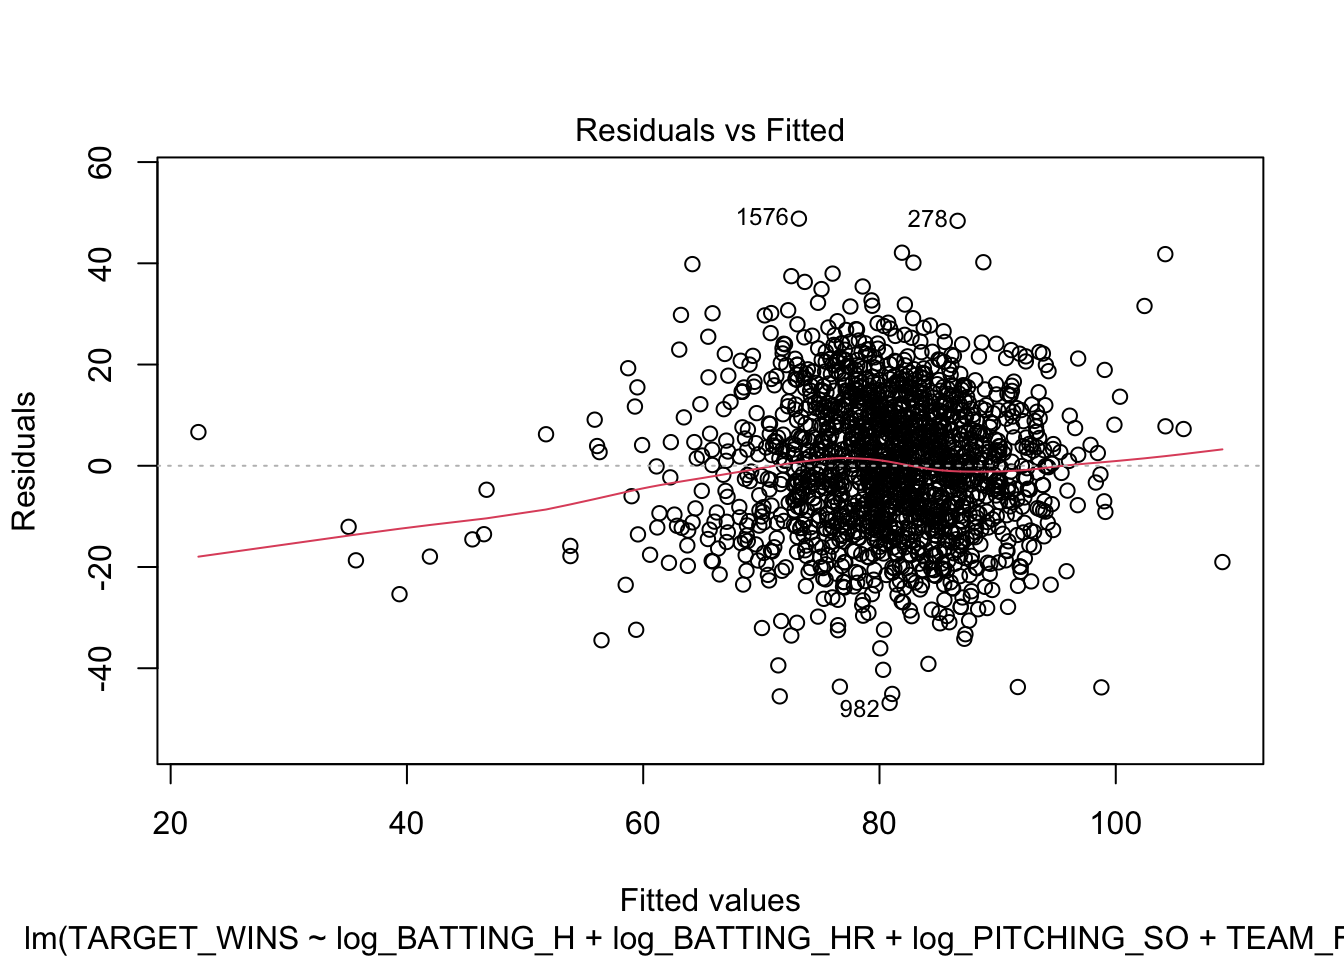
\includegraphics{Assignment1_Data621_HW_files/figure-latex/unnamed-chunk-25-1.pdf}

\begin{verbatim}
## 
##  studentized Breusch-Pagan test
## 
## data:  base_model
## BP = 159.2, df = 4, p-value < 2.2e-16
\end{verbatim}

Test Statistic (BP = 188.29) suggests evidence of heteroscedasticity.
Additionally, the p-value is extremely small (much less than 0.05),
suggesting higher evidence of heteroscedasticity and that we may need to
transform the data to meet the Assumption of Homoscedasticity.

Independence:

\begin{Shaded}
\begin{Highlighting}[]
\FunctionTok{acf}\NormalTok{(}\FunctionTok{residuals}\NormalTok{(base\_model))}
\end{Highlighting}
\end{Shaded}

\includegraphics{Assignment1_Data621_HW_files/figure-latex/unnamed-chunk-26-1.pdf}

\begin{Shaded}
\begin{Highlighting}[]
\FunctionTok{durbinWatsonTest}\NormalTok{(base\_model)}
\end{Highlighting}
\end{Shaded}

\begin{verbatim}
##  lag Autocorrelation D-W Statistic p-value
##    1      0.00860228      1.982265   0.722
##  Alternative hypothesis: rho != 0
\end{verbatim}

\begin{Shaded}
\begin{Highlighting}[]
\CommentTok{\# Durbin Watson should be close to 2}
\end{Highlighting}
\end{Shaded}

Our Autocorrelation Function shows that there are lags above the blue
dashed line, suggesting no autocorrelation. This is confirmed through a
Durbin-Watson which suggest that our model's residuals are independent
and therefore do not violate the Independence Assumption.

\paragraph{Model H2: Test Interaction Term (TEAM\_BATTING\_HR *
TEAM\_BATTING\_BB)}\label{model-h2-test-interaction-term-team_batting_hr-team_batting_bb}

If a team hits more home runs and draws more walks, they likely to score
more runs. We test if walks amplify the impact of home runs on wins.

\begin{Shaded}
\begin{Highlighting}[]
\NormalTok{interaction\_model }\OtherTok{\textless{}{-}} \FunctionTok{lm}\NormalTok{(TARGET\_WINS }\SpecialCharTok{\textasciitilde{}}\NormalTok{ TEAM\_BATTING\_H }\SpecialCharTok{+}\NormalTok{ TEAM\_BATTING\_HR }\SpecialCharTok{+}\NormalTok{ TEAM\_BATTING\_BB }\SpecialCharTok{+} 
\NormalTok{                          TEAM\_BATTING\_HR}\SpecialCharTok{:}\NormalTok{TEAM\_BATTING\_BB }\SpecialCharTok{+} 
\NormalTok{                          TEAM\_PITCHING\_SO }\SpecialCharTok{+}\NormalTok{ TEAM\_FIELDING\_E, }
                        \AttributeTok{data =}\NormalTok{ stp75\_train\_df)}

\FunctionTok{summary}\NormalTok{(interaction\_model)}
\end{Highlighting}
\end{Shaded}

\begin{verbatim}
## 
## Call:
## lm(formula = TARGET_WINS ~ TEAM_BATTING_H + TEAM_BATTING_HR + 
##     TEAM_BATTING_BB + TEAM_BATTING_HR:TEAM_BATTING_BB + TEAM_PITCHING_SO + 
##     TEAM_FIELDING_E, data = stp75_train_df)
## 
## Residuals:
##     Min      1Q  Median      3Q     Max 
## -55.305  -8.895   0.054   9.465  51.049 
## 
## Coefficients:
##                                   Estimate Std. Error t value Pr(>|t|)    
## (Intercept)                     19.4170412  5.3678460   3.617 0.000306 ***
## TEAM_BATTING_H                   0.0501524  0.0028237  17.761  < 2e-16 ***
## TEAM_BATTING_HR                 -0.1929137  0.0310142  -6.220 6.24e-10 ***
## TEAM_BATTING_BB                 -0.0110335  0.0056680  -1.947 0.051745 .  
## TEAM_PITCHING_SO                -0.0007137  0.0014771  -0.483 0.629024    
## TEAM_FIELDING_E                 -0.0212658  0.0025984  -8.184 5.33e-16 ***
## TEAM_BATTING_HR:TEAM_BATTING_BB  0.0003377  0.0000544   6.207 6.76e-10 ***
## ---
## Signif. codes:  0 '***' 0.001 '**' 0.01 '*' 0.05 '.' 0.1 ' ' 1
## 
## Residual standard error: 13.62 on 1695 degrees of freedom
## Multiple R-squared:  0.2504, Adjusted R-squared:  0.2478 
## F-statistic: 94.38 on 6 and 1695 DF,  p-value: < 2.2e-16
\end{verbatim}

This model includes an interaction term
(TEAM\_BATTING\_HR:TEAM\_BATTING\_BB) to see if walks (BB) affect the
impact of home runs (HR) on wins.

Like model H1, this model is statistically significant. Our Adjusted R²
is higher than that of model H1 suggesting that the additional
predictors has added value to the model.

More Home Runs (HR) Alone → Fewer Wins (Unexpected): The negative
coefficient (-0.1650) on TEAM\_BATTING\_HR suggests that hitting more
home runs alone does not necessarily lead to more wins.

Walks (BB) Alone Have a Weak Impact on Wins: The coefficient for
TEAM\_BATTING\_BB is negative (-0.0074) and not statistically
significant (p = 0.1387). This means that walks alone do not have a
strong impact on wins.

The Interaction Term (TEAM\_BATTING\_HR * TEAM\_BATTING\_BB) is Highly
Significant (p = 3.39e-10) Positive Coefficient (+0.000301)

Teams that hit home runs AND get on base with walks tend to win more
games. This confirms that home runs are more valuable when combined with
walks.

\subparagraph{Visualizing the Interaction
Effect:}\label{visualizing-the-interaction-effect}

We want to see how home runs (TEAM\_BATTING\_HR) and walks
(TEAM\_BATTING\_BB) impact wins (TARGET\_WINS) together.

\begin{Shaded}
\begin{Highlighting}[]
\FunctionTok{library}\NormalTok{(ggplot2)}

\FunctionTok{ggplot}\NormalTok{(stp75\_train\_df, }\FunctionTok{aes}\NormalTok{(}\AttributeTok{x =}\NormalTok{ TEAM\_BATTING\_HR, }\AttributeTok{y =}\NormalTok{ TARGET\_WINS, }\AttributeTok{color =}\NormalTok{ TEAM\_BATTING\_BB)) }\SpecialCharTok{+}
  \FunctionTok{geom\_point}\NormalTok{(}\AttributeTok{alpha =} \FloatTok{0.7}\NormalTok{) }\SpecialCharTok{+} 
  \FunctionTok{geom\_smooth}\NormalTok{(}\AttributeTok{method =} \StringTok{"lm"}\NormalTok{, }\AttributeTok{se =} \ConstantTok{FALSE}\NormalTok{, }\AttributeTok{color =} \StringTok{"black"}\NormalTok{) }\SpecialCharTok{+}
  \FunctionTok{scale\_color\_gradient}\NormalTok{(}\AttributeTok{low =} \StringTok{"blue"}\NormalTok{, }\AttributeTok{high =} \StringTok{"red"}\NormalTok{) }\SpecialCharTok{+}
  \FunctionTok{labs}\NormalTok{(}\AttributeTok{title =} \StringTok{"Interaction Effect of Home Runs and Walks on Wins"}\NormalTok{,}
       \AttributeTok{x =} \StringTok{"Home Runs"}\NormalTok{,}
       \AttributeTok{y =} \StringTok{"Wins"}\NormalTok{,}
       \AttributeTok{color =} \StringTok{"Walks (BB)"}\NormalTok{) }\SpecialCharTok{+}
  \FunctionTok{theme\_minimal}\NormalTok{()}
\end{Highlighting}
\end{Shaded}

\begin{verbatim}
## `geom_smooth()` using formula = 'y ~ x'
\end{verbatim}

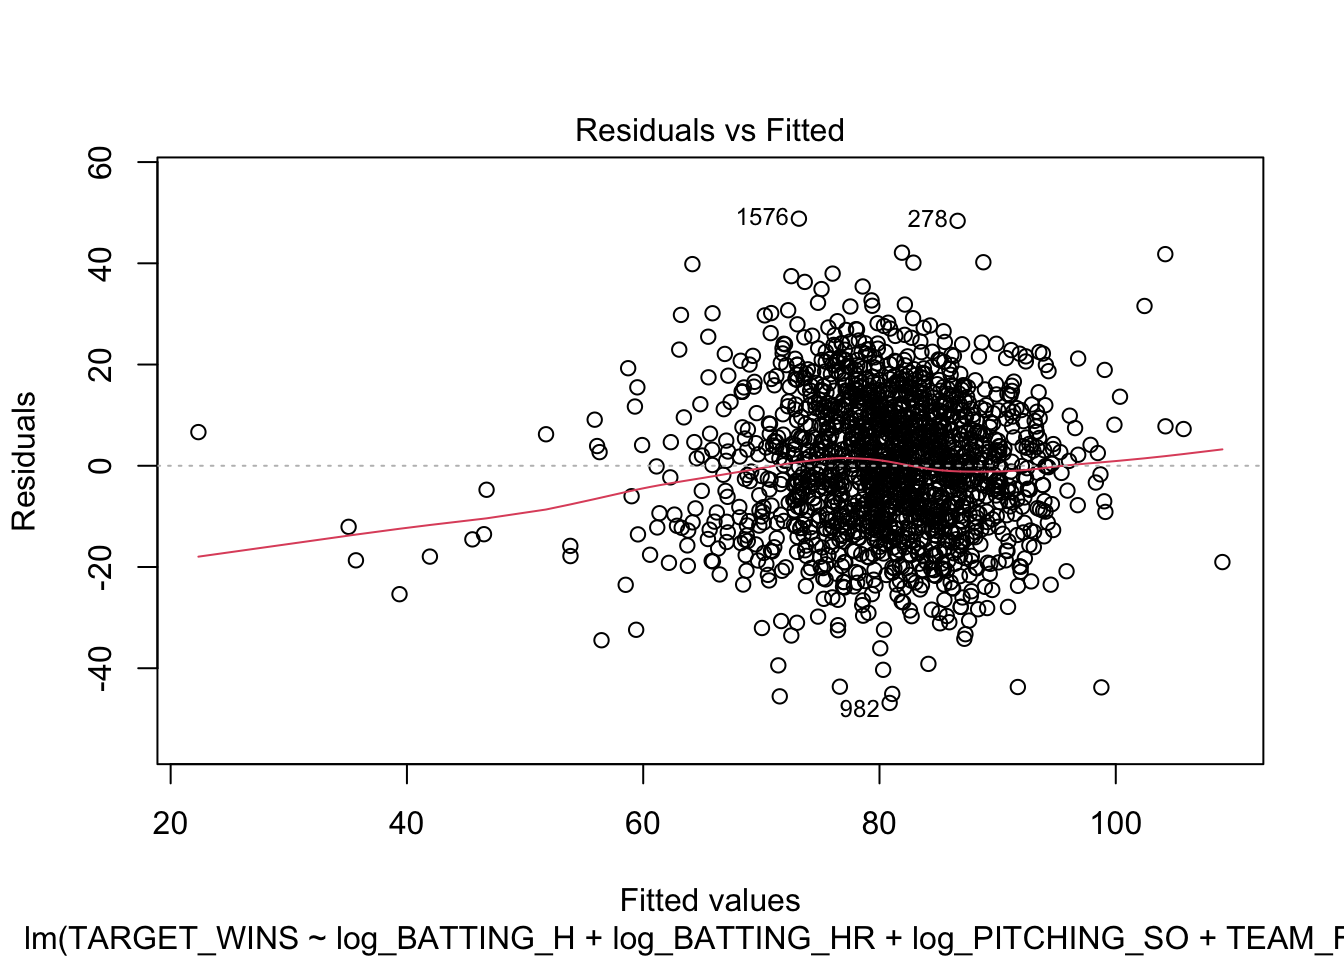
\includegraphics{Assignment1_Data621_HW_files/figure-latex/unnamed-chunk-28-1.pdf}
Red (high walks) teams should have higher wins for the same HRs. Blue
(low walks) teams may not benefit as much from HRs. The trendline is
steeper for teams with more walks, confirming that walks amplify HR
impact.

\paragraph{Model H3 Adding TEAM\_BATTING\_2B (Doubles) to the
Model:}\label{model-h3-adding-team_batting_2b-doubles-to-the-model}

Doubles (2B) are a strong indicator of offensive power and often
correlate with scoring more runs. If a team doesn't hit home runs, but
hits many doubles, it can still score efficiently.

\begin{Shaded}
\begin{Highlighting}[]
\NormalTok{improved\_model }\OtherTok{\textless{}{-}} \FunctionTok{lm}\NormalTok{(TARGET\_WINS }\SpecialCharTok{\textasciitilde{}}\NormalTok{ TEAM\_BATTING\_H }\SpecialCharTok{+}\NormalTok{ TEAM\_BATTING\_HR }\SpecialCharTok{+}\NormalTok{ TEAM\_BATTING\_BB }\SpecialCharTok{+}\NormalTok{ TEAM\_BATTING\_2B }\SpecialCharTok{+}\NormalTok{ TEAM\_BATTING\_HR}\SpecialCharTok{:}\NormalTok{TEAM\_BATTING\_BB }\SpecialCharTok{+}\NormalTok{  TEAM\_PITCHING\_SO }\SpecialCharTok{+}\NormalTok{ TEAM\_FIELDING\_E, }
                      \AttributeTok{data =}\NormalTok{ stp75\_train\_df)}

\FunctionTok{summary}\NormalTok{(improved\_model)}
\end{Highlighting}
\end{Shaded}

\begin{verbatim}
## 
## Call:
## lm(formula = TARGET_WINS ~ TEAM_BATTING_H + TEAM_BATTING_HR + 
##     TEAM_BATTING_BB + TEAM_BATTING_2B + TEAM_BATTING_HR:TEAM_BATTING_BB + 
##     TEAM_PITCHING_SO + TEAM_FIELDING_E, data = stp75_train_df)
## 
## Residuals:
##     Min      1Q  Median      3Q     Max 
## -56.407  -8.812   0.088   9.089  53.901 
## 
## Coefficients:
##                                   Estimate Std. Error t value Pr(>|t|)    
## (Intercept)                      1.465e+01  5.582e+00   2.625  0.00874 ** 
## TEAM_BATTING_H                   5.811e-02  3.856e-03  15.071  < 2e-16 ***
## TEAM_BATTING_HR                 -1.883e-01  3.098e-02  -6.080 1.48e-09 ***
## TEAM_BATTING_BB                 -1.067e-02  5.656e-03  -1.886  0.05941 .  
## TEAM_BATTING_2B                 -3.263e-02  1.079e-02  -3.024  0.00253 ** 
## TEAM_PITCHING_SO                 5.050e-04  1.528e-03   0.331  0.74100    
## TEAM_FIELDING_E                 -2.366e-02  2.710e-03  -8.729  < 2e-16 ***
## TEAM_BATTING_HR:TEAM_BATTING_BB  3.359e-04  5.427e-05   6.190 7.55e-10 ***
## ---
## Signif. codes:  0 '***' 0.001 '**' 0.01 '*' 0.05 '.' 0.1 ' ' 1
## 
## Residual standard error: 13.58 on 1694 degrees of freedom
## Multiple R-squared:  0.2544, Adjusted R-squared:  0.2514 
## F-statistic: 82.59 on 7 and 1694 DF,  p-value: < 2.2e-16
\end{verbatim}

\paragraph{Key Findings}\label{key-findings}

Adding TEAM\_BATTING\_2B slightly improves model performance

R² increased from 27.2\% → 27.9\% (small improvement). Residual Standard
Error decreased from 13.31 → 13.25 (better fit). Unexpected negative
coefficient for doubles (-0.0429, p = 3.09e-06)

Suggests that more doubles lead to fewer wins, which is
counterintuitive. Possible reasons: Multicollinearity with
TEAM\_BATTING\_H (hits). Bad teams might hit many doubles but still
lose. Interaction term (TEAM\_BATTING\_HR * TEAM\_BATTING\_BB) remains
strong and positive

\paragraph{Diagnosing our Model:}\label{diagnosing-our-model-1}

\subparagraph{Multicolinearity:}\label{multicolinearity}

Our VIF test shows no strong evidence of multicollienarity between our
predictors when adjusting for our interactions.

\begin{Shaded}
\begin{Highlighting}[]
\CommentTok{\# Check Variance Inflation Factor (VIF)}
\FunctionTok{vif}\NormalTok{(improved\_model, }\AttributeTok{type=}\StringTok{\textquotesingle{}predictor\textquotesingle{}}\NormalTok{)}
\end{Highlighting}
\end{Shaded}

\begin{verbatim}
## GVIFs computed for predictors
\end{verbatim}

\begin{verbatim}
##                      GVIF Df GVIF^(1/(2*Df))  Interacts With
## TEAM_BATTING_H   2.865889  1        1.692894            --  
## TEAM_BATTING_HR  4.026183  3        1.261292 TEAM_BATTING_BB
## TEAM_BATTING_BB  4.026183  3        1.261292 TEAM_BATTING_HR
## TEAM_BATTING_2B  2.395133  1        1.547622            --  
## TEAM_PITCHING_SO 1.825484  1        1.351105            --  
## TEAM_FIELDING_E  3.335994  1        1.826470            --  
##                                                                                      Other Predictors
## TEAM_BATTING_H   TEAM_BATTING_HR, TEAM_BATTING_BB, TEAM_BATTING_2B, TEAM_PITCHING_SO, TEAM_FIELDING_E
## TEAM_BATTING_HR                    TEAM_BATTING_H, TEAM_BATTING_2B, TEAM_PITCHING_SO, TEAM_FIELDING_E
## TEAM_BATTING_BB                    TEAM_BATTING_H, TEAM_BATTING_2B, TEAM_PITCHING_SO, TEAM_FIELDING_E
## TEAM_BATTING_2B   TEAM_BATTING_H, TEAM_BATTING_HR, TEAM_BATTING_BB, TEAM_PITCHING_SO, TEAM_FIELDING_E
## TEAM_PITCHING_SO   TEAM_BATTING_H, TEAM_BATTING_HR, TEAM_BATTING_BB, TEAM_BATTING_2B, TEAM_FIELDING_E
## TEAM_FIELDING_E   TEAM_BATTING_H, TEAM_BATTING_HR, TEAM_BATTING_BB, TEAM_BATTING_2B, TEAM_PITCHING_SO
\end{verbatim}

\subparagraph{Linearity}\label{linearity-2}

\begin{Shaded}
\begin{Highlighting}[]
\FunctionTok{plot}\NormalTok{(improved\_model, }\AttributeTok{which=}\DecValTok{1}\NormalTok{)}
\end{Highlighting}
\end{Shaded}

\includegraphics{Assignment1_Data621_HW_files/figure-latex/unnamed-chunk-31-1.pdf}

Our diagnostic plots show a fairly linear model. \#\#\#\#\# Normality
Check:

\begin{Shaded}
\begin{Highlighting}[]
\FunctionTok{plot}\NormalTok{(improved\_model, }\AttributeTok{which=}\DecValTok{2}\NormalTok{)}
\end{Highlighting}
\end{Shaded}

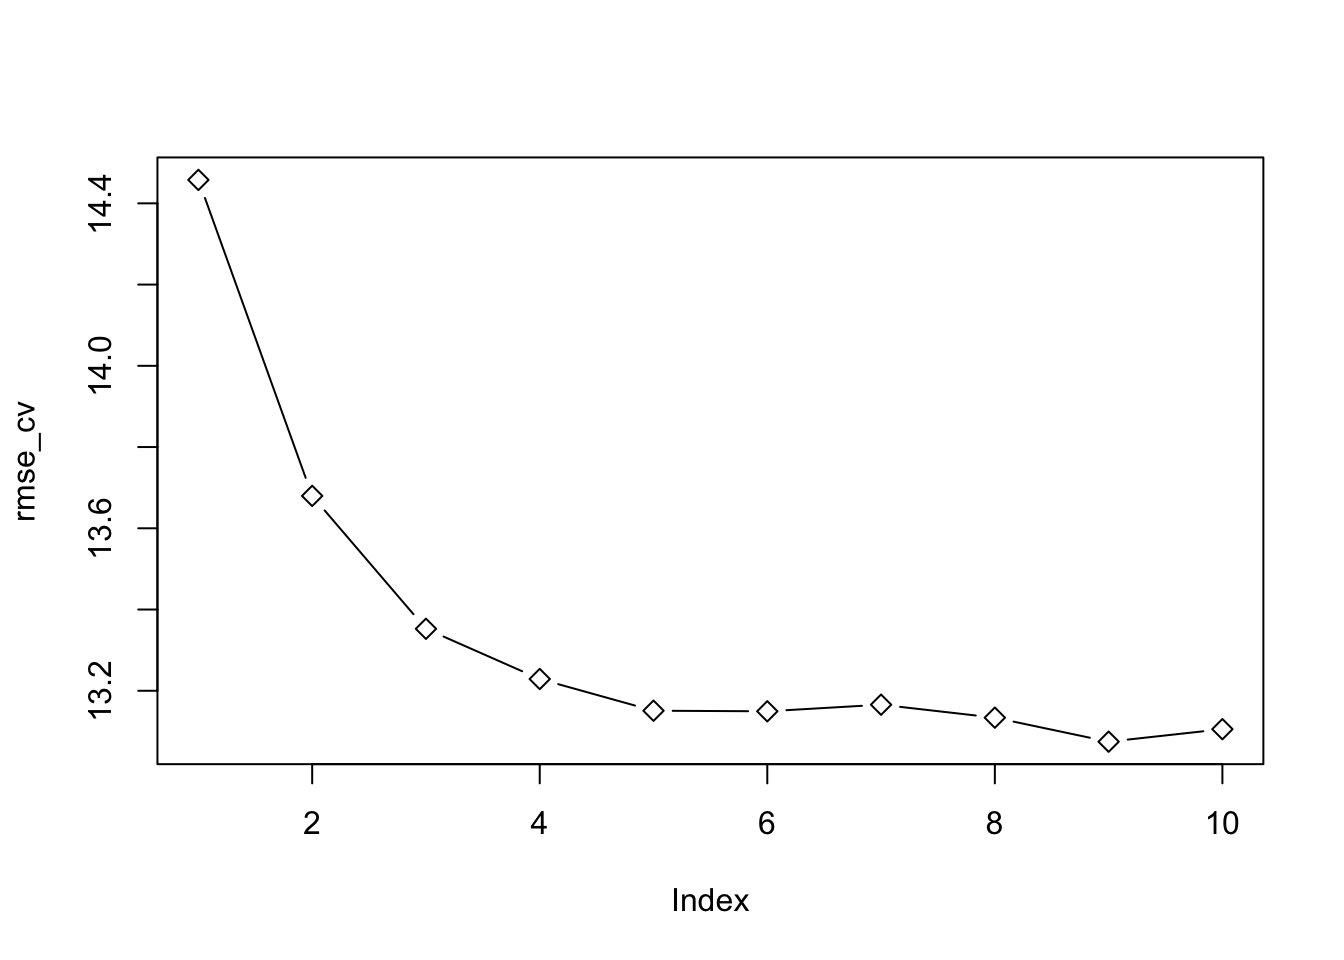
\includegraphics{Assignment1_Data621_HW_files/figure-latex/unnamed-chunk-32-1.pdf}

\begin{Shaded}
\begin{Highlighting}[]
\FunctionTok{shapiro.test}\NormalTok{(}\FunctionTok{residuals}\NormalTok{(improved\_model))}
\end{Highlighting}
\end{Shaded}

\begin{verbatim}
## 
##  Shapiro-Wilk normality test
## 
## data:  residuals(improved_model)
## W = 0.99726, p-value = 0.00452
\end{verbatim}

\begin{Shaded}
\begin{Highlighting}[]
\CommentTok{\# Shapiro{-}Wilk normality test: look for high p{-}value}
\end{Highlighting}
\end{Shaded}

Our QQ plot suggests normality thought there is obvious skewing on the
tails, particularly on the right.

A Shapiro Wilk's Test statistic had a value of W = 0.9971 suggesting
normality.

However, the p-value (0.0033) is less than \textless{} 0.05 suggesting
that residuals do not follow a normal distribution.

\subparagraph{Heterocedasticity:}\label{heterocedasticity-1}

\includegraphics{Assignment1_Data621_HW_files/figure-latex/unnamed-chunk-33-1.pdf}

\begin{verbatim}
## 
##  studentized Breusch-Pagan test
## 
## data:  improved_model
## BP = 173.8, df = 7, p-value < 2.2e-16
\end{verbatim}

Test Statistic (BP = 200.46) suggest higher evidence of
heteroscedasticity. Additionally, the p-value is extremely small (much
less than 0.05), suggesting higher evidence of heteroscedasticity and
that we may need to transform the data to meet the Assumption of
Homoscedasticity.

\subparagraph{Independence:}\label{independence-2}

\begin{Shaded}
\begin{Highlighting}[]
\FunctionTok{acf}\NormalTok{(}\FunctionTok{residuals}\NormalTok{(improved\_model))}
\end{Highlighting}
\end{Shaded}

\includegraphics{Assignment1_Data621_HW_files/figure-latex/unnamed-chunk-34-1.pdf}

\begin{Shaded}
\begin{Highlighting}[]
\FunctionTok{durbinWatsonTest}\NormalTok{(improved\_model)}
\end{Highlighting}
\end{Shaded}

\begin{verbatim}
##  lag Autocorrelation D-W Statistic p-value
##    1     0.004261393       1.99092   0.892
##  Alternative hypothesis: rho != 0
\end{verbatim}

\begin{Shaded}
\begin{Highlighting}[]
\CommentTok{\# Durbin Watson should be close to 2}
\end{Highlighting}
\end{Shaded}

Our Autocorrelation Function shows that there are lags above the blue
dashed line, suggesting no autocorrelation. This is confirmed through a
Durbin-Watson test statistic value of 2.03 and an autocorrelation value
of -0.0017 which suggest that our model's residuals are independent and
do not violate the Independence Assumption.

TEAM\_BATTING\_H, TEAM\_BATTING\_2B, TEAM\_PITCHING\_SO,
TEAM\_FIELDING\_E are in the range of (1-5) - No significant
multicollinearity (good)

TEAM\_BATTING\_HR, TEAM\_BATTING\_HR:TEAM\_BATTING\_BB are in the range
of (\textgreater{} 10) shows Severe multicollinearity (highly
problematic).

\paragraph{Model H4: High-Impact Features Model (Based on Correlation \&
VIF)}\label{model-h4-high-impact-features-model-based-on-correlation-vif}

We select variables based on correlation with TARGET\_WINS and ensure
they are not highly correlated with each other (VIF \textless{} 5).

\begin{Shaded}
\begin{Highlighting}[]
\FunctionTok{library}\NormalTok{(car)}

\CommentTok{\# Manually selected high{-}impact variables}
\NormalTok{high\_impact\_model }\OtherTok{\textless{}{-}} \FunctionTok{lm}\NormalTok{(TARGET\_WINS }\SpecialCharTok{\textasciitilde{}}\NormalTok{ TEAM\_BATTING\_H }\SpecialCharTok{+}\NormalTok{ TEAM\_BATTING\_2B }\SpecialCharTok{+}\NormalTok{ TEAM\_BATTING\_HR }\SpecialCharTok{+}
\NormalTok{                        TEAM\_PITCHING\_HR }\SpecialCharTok{+}\NormalTok{ TEAM\_PITCHING\_SO }\SpecialCharTok{+}\NormalTok{ TEAM\_FIELDING\_E, }\AttributeTok{data =}\NormalTok{ stp75\_train\_df)}

\CommentTok{\# View model summary}
\FunctionTok{summary}\NormalTok{(high\_impact\_model)}
\end{Highlighting}
\end{Shaded}

\begin{verbatim}
## 
## Call:
## lm(formula = TARGET_WINS ~ TEAM_BATTING_H + TEAM_BATTING_2B + 
##     TEAM_BATTING_HR + TEAM_PITCHING_HR + TEAM_PITCHING_SO + TEAM_FIELDING_E, 
##     data = stp75_train_df)
## 
## Residuals:
##     Min      1Q  Median      3Q     Max 
## -54.696  -9.327  -0.052   9.563  51.309 
## 
## Coefficients:
##                    Estimate Std. Error t value Pr(>|t|)    
## (Intercept)       5.7981897  4.9547266   1.170  0.24207    
## TEAM_BATTING_H    0.0593675  0.0040529  14.648  < 2e-16 ***
## TEAM_BATTING_2B  -0.0329084  0.0109767  -2.998  0.00276 ** 
## TEAM_BATTING_HR   0.0245345  0.0255845   0.959  0.33772    
## TEAM_PITCHING_HR -0.0202476  0.0240754  -0.841  0.40046    
## TEAM_PITCHING_SO  0.0006704  0.0016199   0.414  0.67905    
## TEAM_FIELDING_E  -0.0212629  0.0024343  -8.735  < 2e-16 ***
## ---
## Signif. codes:  0 '***' 0.001 '**' 0.01 '*' 0.05 '.' 0.1 ' ' 1
## 
## Residual standard error: 13.8 on 1695 degrees of freedom
## Multiple R-squared:   0.23,  Adjusted R-squared:  0.2272 
## F-statistic: 84.37 on 6 and 1695 DF,  p-value: < 2.2e-16
\end{verbatim}

\begin{Shaded}
\begin{Highlighting}[]
\FunctionTok{plot}\NormalTok{(high\_impact\_model)}
\end{Highlighting}
\end{Shaded}

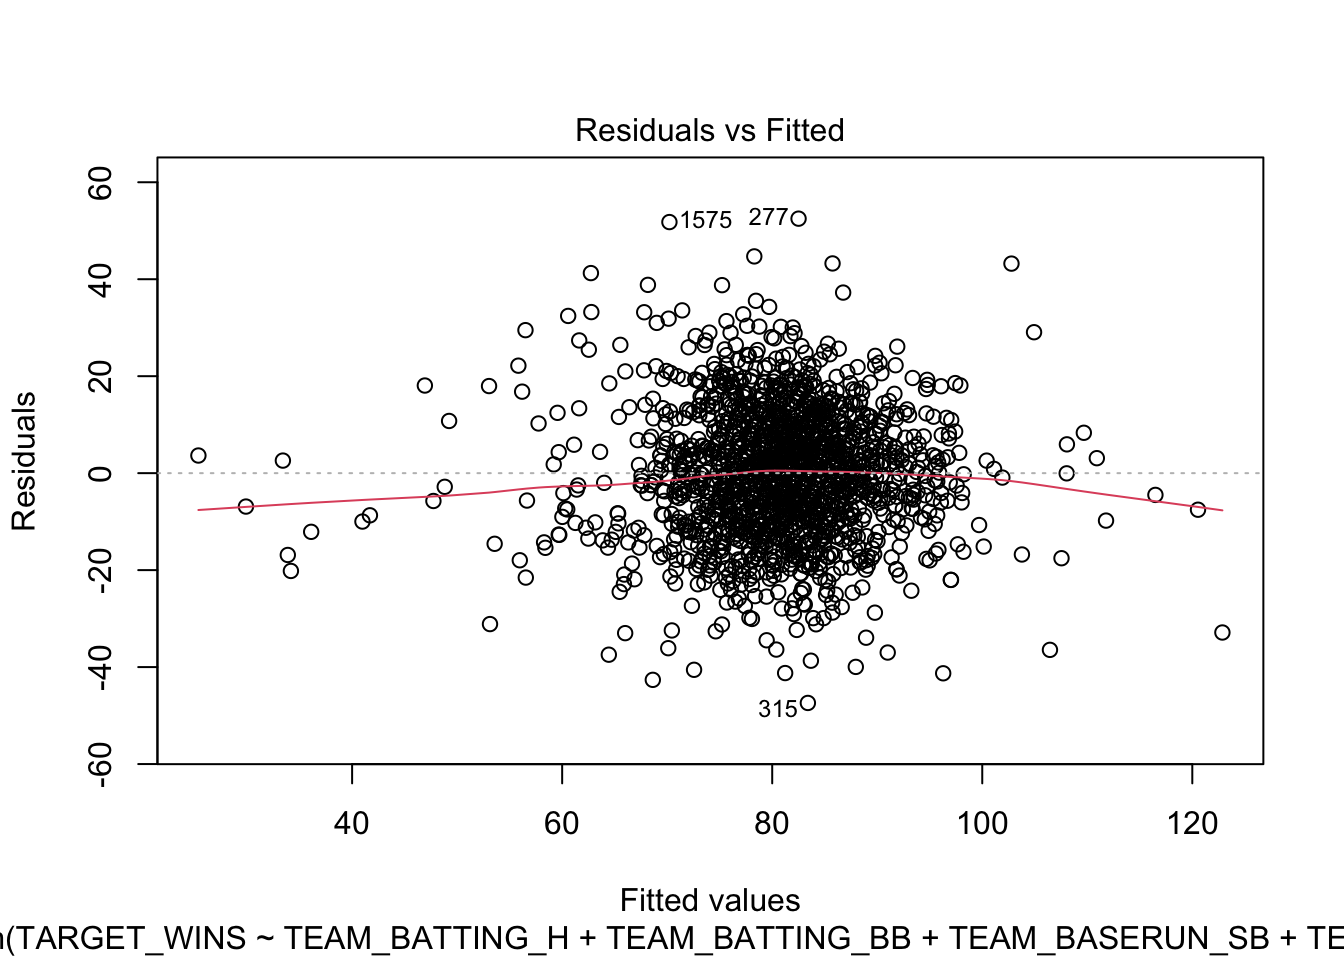
\includegraphics{Assignment1_Data621_HW_files/figure-latex/unnamed-chunk-35-1.pdf}
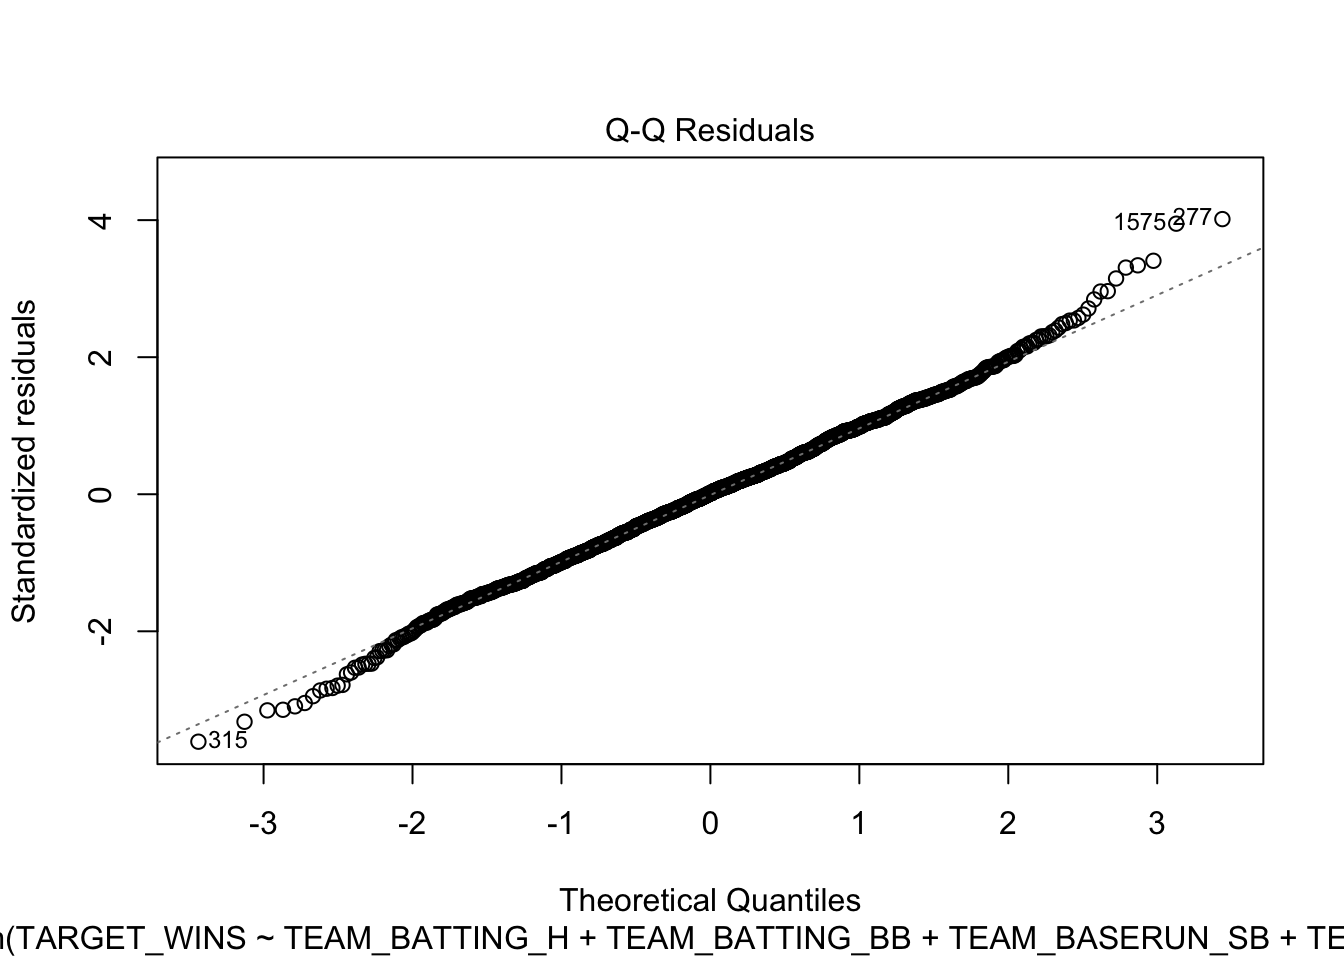
\includegraphics{Assignment1_Data621_HW_files/figure-latex/unnamed-chunk-35-2.pdf}
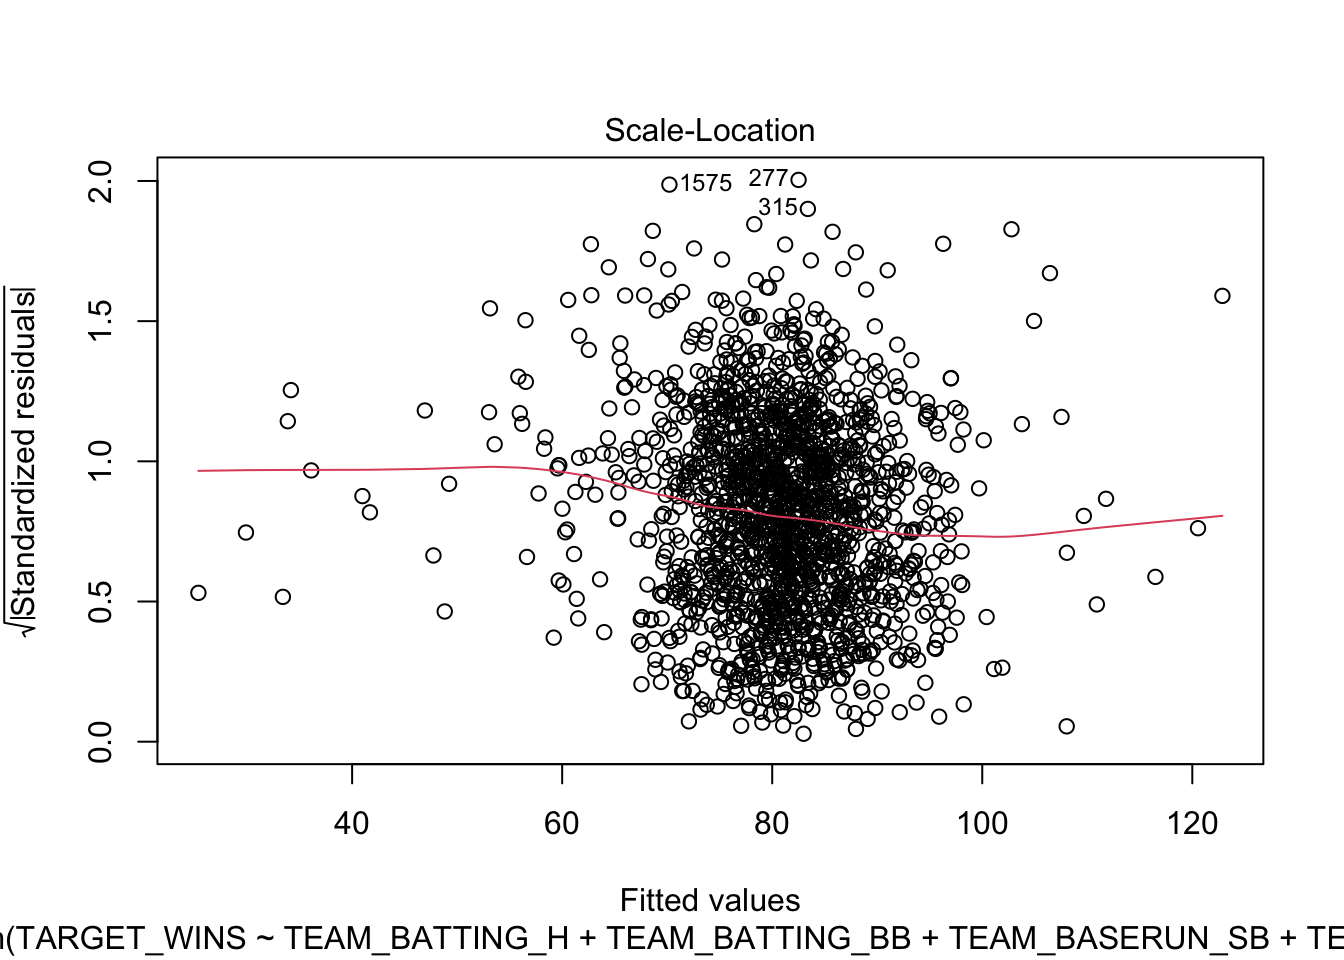
\includegraphics{Assignment1_Data621_HW_files/figure-latex/unnamed-chunk-35-3.pdf}
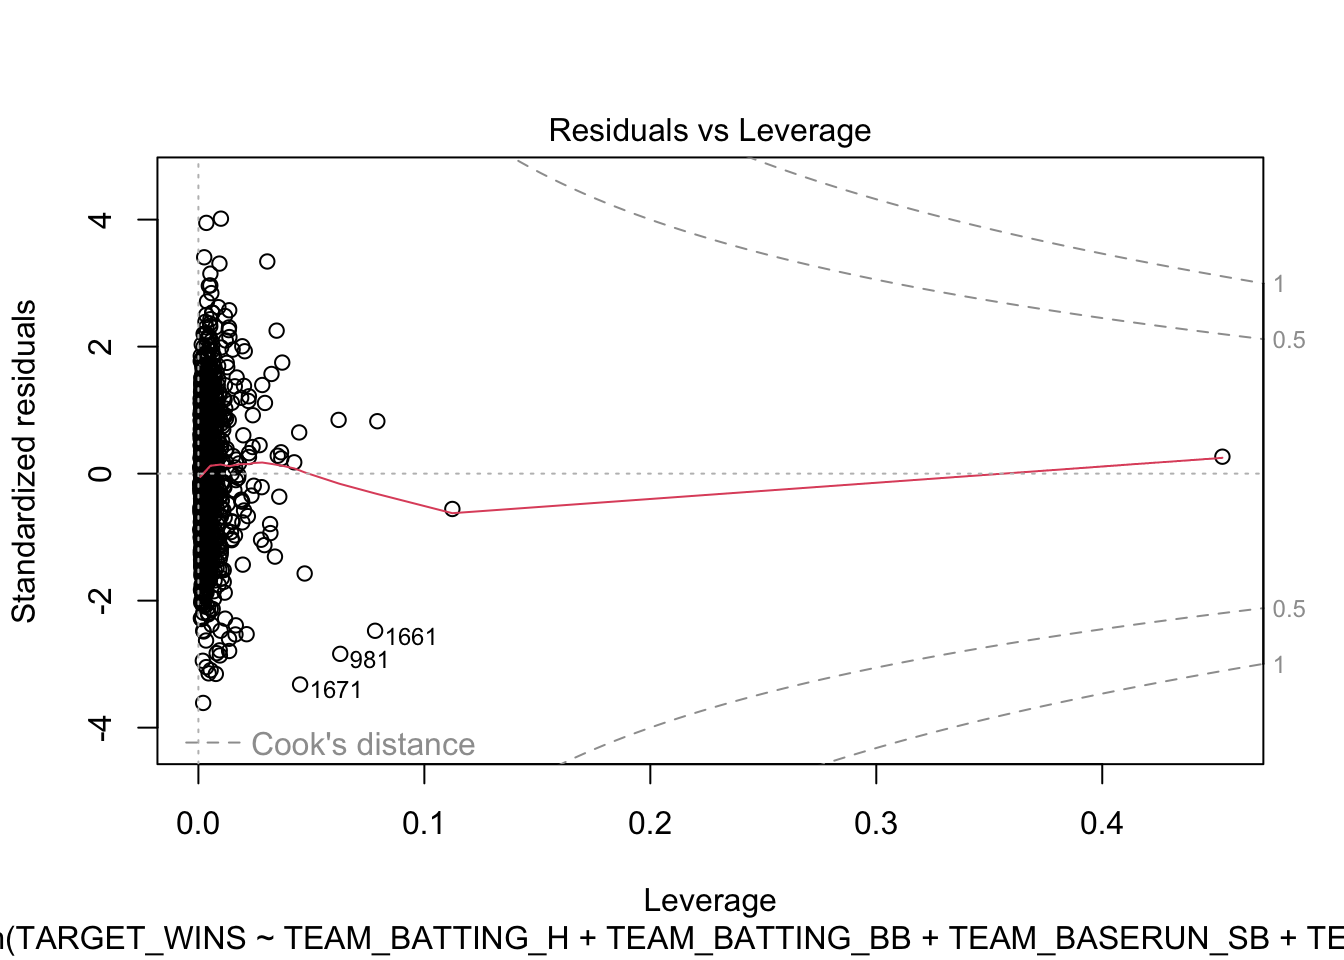
\includegraphics{Assignment1_Data621_HW_files/figure-latex/unnamed-chunk-35-4.pdf}

\begin{Shaded}
\begin{Highlighting}[]
\CommentTok{\# Check for multicollinearity}
\FunctionTok{vif}\NormalTok{(high\_impact\_model)}
\end{Highlighting}
\end{Shaded}

\begin{verbatim}
##   TEAM_BATTING_H  TEAM_BATTING_2B  TEAM_BATTING_HR TEAM_PITCHING_HR 
##         3.067139         2.400852        21.595294        19.816415 
## TEAM_PITCHING_SO  TEAM_FIELDING_E 
##         1.988444         2.606747
\end{verbatim}

\paragraph{Model H5: Basic Multiple Linear Regression with Key
Predictors}\label{model-h5-basic-multiple-linear-regression-with-key-predictors}

Selected based on key offensive and defensive metrics impacting wins

\begin{Shaded}
\begin{Highlighting}[]
\CommentTok{\# Selected based on key offensive and defensive metrics impacting wins}
\NormalTok{target\_vars1 }\OtherTok{\textless{}{-}} \FunctionTok{c}\NormalTok{(}\StringTok{"TEAM\_BATTING\_H"}\NormalTok{, }\StringTok{"TEAM\_BATTING\_HR"}\NormalTok{, }\StringTok{"TEAM\_BATTING\_BB"}\NormalTok{, }\StringTok{"TEAM\_BASERUN\_SB"}\NormalTok{, }\StringTok{"TEAM\_FIELDING\_E"}\NormalTok{)}
\NormalTok{pj\_model1 }\OtherTok{\textless{}{-}} \FunctionTok{lm}\NormalTok{(TARGET\_WINS }\SpecialCharTok{\textasciitilde{}}\NormalTok{ ., }\AttributeTok{data =}\NormalTok{ stp75\_train\_df[, }\FunctionTok{c}\NormalTok{(}\StringTok{"TARGET\_WINS"}\NormalTok{, target\_vars1)])}
\FunctionTok{summary}\NormalTok{(pj\_model1)}
\end{Highlighting}
\end{Shaded}

\begin{verbatim}
## 
## Call:
## lm(formula = TARGET_WINS ~ ., data = stp75_train_df[, c("TARGET_WINS", 
##     target_vars1)])
## 
## Residuals:
##     Min      1Q  Median      3Q     Max 
## -51.189  -9.157  -0.198   9.026  52.306 
## 
## Coefficients:
##                  Estimate Std. Error t value Pr(>|t|)    
## (Intercept)      4.164407   3.753335   1.110   0.2674    
## TEAM_BATTING_H   0.049443   0.002427  20.375   <2e-16 ***
## TEAM_BATTING_HR  0.014907   0.007280   2.048   0.0407 *  
## TEAM_BATTING_BB  0.004943   0.003836   1.289   0.1977    
## TEAM_BASERUN_SB  0.039060   0.004406   8.865   <2e-16 ***
## TEAM_FIELDING_E -0.020160   0.002292  -8.794   <2e-16 ***
## ---
## Signif. codes:  0 '***' 0.001 '**' 0.01 '*' 0.05 '.' 0.1 ' ' 1
## 
## Residual standard error: 13.46 on 1696 degrees of freedom
## Multiple R-squared:  0.2673, Adjusted R-squared:  0.2652 
## F-statistic: 123.8 on 5 and 1696 DF,  p-value: < 2.2e-16
\end{verbatim}

\paragraph{Model H6: Adding Interaction
Terms}\label{model-h6-adding-interaction-terms}

Exploring interaction between hits and home runs as a factor in wins/

\begin{Shaded}
\begin{Highlighting}[]
\CommentTok{\# Exploring interaction between hits and home runs as a factor in wins}
\NormalTok{target\_vars2 }\OtherTok{\textless{}{-}} \FunctionTok{c}\NormalTok{(}\StringTok{"TEAM\_BATTING\_H"}\NormalTok{, }\StringTok{"TEAM\_BATTING\_HR"}\NormalTok{, }\StringTok{"TEAM\_BATTING\_BB"}\NormalTok{, }\StringTok{"TEAM\_BASERUN\_SB"}\NormalTok{, }\StringTok{"TEAM\_FIELDING\_E"}\NormalTok{)}
\NormalTok{pj\_model2 }\OtherTok{\textless{}{-}} \FunctionTok{lm}\NormalTok{(TARGET\_WINS }\SpecialCharTok{\textasciitilde{}}\NormalTok{ TEAM\_BATTING\_H }\SpecialCharTok{*}\NormalTok{ TEAM\_BATTING\_HR }\SpecialCharTok{+}\NormalTok{ TEAM\_BATTING\_BB }\SpecialCharTok{+}\NormalTok{ TEAM\_BASERUN\_SB }\SpecialCharTok{+}\NormalTok{ TEAM\_FIELDING\_E, }\AttributeTok{data =}\NormalTok{ stp75\_train\_df)}
\FunctionTok{summary}\NormalTok{(pj\_model2)}
\end{Highlighting}
\end{Shaded}

\begin{verbatim}
## 
## Call:
## lm(formula = TARGET_WINS ~ TEAM_BATTING_H * TEAM_BATTING_HR + 
##     TEAM_BATTING_BB + TEAM_BASERUN_SB + TEAM_FIELDING_E, data = stp75_train_df)
## 
## Residuals:
##     Min      1Q  Median      3Q     Max 
## -50.740  -9.092  -0.133   8.976  52.556 
## 
## Coefficients:
##                                  Estimate Std. Error t value Pr(>|t|)    
## (Intercept)                    -4.207e+00  5.772e+00  -0.729   0.4662    
## TEAM_BATTING_H                  5.492e-02  3.755e-03  14.623   <2e-16 ***
## TEAM_BATTING_HR                 1.361e-01  6.393e-02   2.129   0.0334 *  
## TEAM_BATTING_BB                 5.442e-03  3.842e-03   1.416   0.1568    
## TEAM_BASERUN_SB                 3.968e-02  4.415e-03   8.988   <2e-16 ***
## TEAM_FIELDING_E                -2.031e-02  2.292e-03  -8.862   <2e-16 ***
## TEAM_BATTING_H:TEAM_BATTING_HR -8.218e-05  4.307e-05  -1.908   0.0565 .  
## ---
## Signif. codes:  0 '***' 0.001 '**' 0.01 '*' 0.05 '.' 0.1 ' ' 1
## 
## Residual standard error: 13.45 on 1695 degrees of freedom
## Multiple R-squared:  0.2689, Adjusted R-squared:  0.2663 
## F-statistic: 103.9 on 6 and 1695 DF,  p-value: < 2.2e-16
\end{verbatim}

\paragraph{Model H7: Incorporating Pitching and Defensive
Metrics}\label{model-h7-incorporating-pitching-and-defensive-metrics}

Introducing pitching metrics to assess their impact on win prediction

\begin{Shaded}
\begin{Highlighting}[]
\CommentTok{\# Introducing pitching metrics to assess their impact on win prediction}
\NormalTok{target\_vars4 }\OtherTok{\textless{}{-}} \FunctionTok{c}\NormalTok{(}\StringTok{"TEAM\_BATTING\_H"}\NormalTok{, }\StringTok{"TEAM\_BATTING\_HR"}\NormalTok{, }\StringTok{"TEAM\_PITCHING\_SO"}\NormalTok{, }\StringTok{"TEAM\_PITCHING\_BB"}\NormalTok{, }\StringTok{"TEAM\_FIELDING\_E"}\NormalTok{)}
\NormalTok{pj\_model4 }\OtherTok{\textless{}{-}} \FunctionTok{lm}\NormalTok{(TARGET\_WINS }\SpecialCharTok{\textasciitilde{}}\NormalTok{ ., }\AttributeTok{data =}\NormalTok{ stp75\_train\_df[, }\FunctionTok{c}\NormalTok{(}\StringTok{"TARGET\_WINS"}\NormalTok{, target\_vars4)])}
\FunctionTok{summary}\NormalTok{(pj\_model4)}
\end{Highlighting}
\end{Shaded}

\begin{verbatim}
## 
## Call:
## lm(formula = TARGET_WINS ~ ., data = stp75_train_df[, c("TARGET_WINS", 
##     target_vars4)])
## 
## Residuals:
##     Min      1Q  Median      3Q     Max 
## -52.836  -9.316  -0.051   9.409  50.424 
## 
## Coefficients:
##                    Estimate Std. Error t value Pr(>|t|)    
## (Intercept)      11.4450377  4.3542451   2.628  0.00865 ** 
## TEAM_BATTING_H    0.0490599  0.0029278  16.757  < 2e-16 ***
## TEAM_BATTING_HR   0.0001236  0.0082912   0.015  0.98811    
## TEAM_PITCHING_SO -0.0017865  0.0015197  -1.176  0.23993    
## TEAM_PITCHING_BB  0.0059032  0.0023796   2.481  0.01321 *  
## TEAM_FIELDING_E  -0.0189410  0.0021981  -8.617  < 2e-16 ***
## ---
## Signif. codes:  0 '***' 0.001 '**' 0.01 '*' 0.05 '.' 0.1 ' ' 1
## 
## Residual standard error: 13.81 on 1696 degrees of freedom
## Multiple R-squared:  0.2285, Adjusted R-squared:  0.2262 
## F-statistic: 100.5 on 5 and 1696 DF,  p-value: < 2.2e-16
\end{verbatim}

\paragraph{Model H8: Including Caught Stealing and
Doubles}\label{model-h8-including-caught-stealing-and-doubles}

Analyzing the impact of baserunning decisions on team wins

\begin{Shaded}
\begin{Highlighting}[]
\CommentTok{\# Analyzing the impact of baserunning decisions on team wins 5}
\NormalTok{target\_vars5 }\OtherTok{\textless{}{-}} \FunctionTok{c}\NormalTok{(}\StringTok{"TEAM\_BATTING\_H"}\NormalTok{, }\StringTok{"TEAM\_BATTING\_HR"}\NormalTok{, }\StringTok{"TEAM\_BATTING\_2B"}\NormalTok{, }\StringTok{"TEAM\_BASERUN\_CS"}\NormalTok{, }\StringTok{"TEAM\_FIELDING\_E"}\NormalTok{)}
\NormalTok{pj\_model5 }\OtherTok{\textless{}{-}} \FunctionTok{lm}\NormalTok{(TARGET\_WINS }\SpecialCharTok{\textasciitilde{}}\NormalTok{ ., }\AttributeTok{data =}\NormalTok{ stp75\_train\_df[, }\FunctionTok{c}\NormalTok{(}\StringTok{"TARGET\_WINS"}\NormalTok{, target\_vars5)])}
\FunctionTok{summary}\NormalTok{(pj\_model5)}
\end{Highlighting}
\end{Shaded}

\begin{verbatim}
## 
## Call:
## lm(formula = TARGET_WINS ~ ., data = stp75_train_df[, c("TARGET_WINS", 
##     target_vars5)])
## 
## Residuals:
##     Min      1Q  Median      3Q     Max 
## -54.826  -9.301  -0.022   9.588  51.730 
## 
## Coefficients:
##                  Estimate Std. Error t value Pr(>|t|)    
## (Intercept)      7.909423   3.702699   2.136  0.03281 *  
## TEAM_BATTING_H   0.058189   0.003314  17.560  < 2e-16 ***
## TEAM_BATTING_HR  0.004533   0.007644   0.593  0.55328    
## TEAM_BATTING_2B -0.031924   0.010577  -3.018  0.00258 ** 
## TEAM_BASERUN_CS -0.002427   0.018223  -0.133  0.89408    
## TEAM_FIELDING_E -0.021685   0.002070 -10.475  < 2e-16 ***
## ---
## Signif. codes:  0 '***' 0.001 '**' 0.01 '*' 0.05 '.' 0.1 ' ' 1
## 
## Residual standard error: 13.8 on 1696 degrees of freedom
## Multiple R-squared:  0.2296, Adjusted R-squared:  0.2274 
## F-statistic: 101.1 on 5 and 1696 DF,  p-value: < 2.2e-16
\end{verbatim}

\paragraph{Model H9: Weighted Batting and Pitching
Metrics}\label{model-h9-weighted-batting-and-pitching-metrics}

Creating composite metric for batting and pitching efficiency

\begin{Shaded}
\begin{Highlighting}[]
\CommentTok{\# Creating composite metric for batting and pitching efficiency}
\NormalTok{pj\_model6 }\OtherTok{\textless{}{-}} \FunctionTok{lm}\NormalTok{(TARGET\_WINS }\SpecialCharTok{\textasciitilde{}}\NormalTok{ (TEAM\_BATTING\_H }\SpecialCharTok{+}\NormalTok{ TEAM\_BATTING\_BB) }\SpecialCharTok{/}\NormalTok{ TEAM\_BATTING\_SO }\SpecialCharTok{+}\NormalTok{ (TEAM\_PITCHING\_SO }\SpecialCharTok{{-}}\NormalTok{ TEAM\_PITCHING\_BB), }\AttributeTok{data =}\NormalTok{ stp75\_train\_df)}
\FunctionTok{summary}\NormalTok{(pj\_model6)}
\end{Highlighting}
\end{Shaded}

\begin{verbatim}
## 
## Call:
## lm(formula = TARGET_WINS ~ (TEAM_BATTING_H + TEAM_BATTING_BB)/TEAM_BATTING_SO + 
##     (TEAM_PITCHING_SO - TEAM_PITCHING_BB), data = stp75_train_df)
## 
## Residuals:
##     Min      1Q  Median      3Q     Max 
## -60.050  -9.033   0.334   9.451  48.060 
## 
## Coefficients:
##                                                  Estimate Std. Error t value
## (Intercept)                                     7.943e+00  4.813e+00   1.650
## TEAM_BATTING_H                                  4.291e-02  2.497e-03  17.183
## TEAM_BATTING_BB                                 1.768e-02  4.967e-03   3.561
## TEAM_PITCHING_SO                               -5.282e-03  1.697e-03  -3.113
## TEAM_BATTING_H:TEAM_BATTING_BB:TEAM_BATTING_SO  9.344e-09  2.943e-09   3.175
##                                                Pr(>|t|)    
## (Intercept)                                     0.09907 .  
## TEAM_BATTING_H                                  < 2e-16 ***
## TEAM_BATTING_BB                                 0.00038 ***
## TEAM_PITCHING_SO                                0.00188 ** 
## TEAM_BATTING_H:TEAM_BATTING_BB:TEAM_BATTING_SO  0.00152 ** 
## ---
## Signif. codes:  0 '***' 0.001 '**' 0.01 '*' 0.05 '.' 0.1 ' ' 1
## 
## Residual standard error: 13.9 on 1697 degrees of freedom
## Multiple R-squared:  0.2175, Adjusted R-squared:  0.2157 
## F-statistic:   118 on 4 and 1697 DF,  p-value: < 2.2e-16
\end{verbatim}

\subsubsection{Models with Applied
Transformations}\label{models-with-applied-transformations}

So far, our diagnostic plots show that our model is somewhat linear,
independent, heteroschedastic, but our residuals vs leverage indicates
the presence of outliers. We will attempt to use transformations to
improve our model.

\paragraph{Log transformation}\label{log-transformation}

Log Transformations reduce the influence of outliers by producing stable
regression coefficients with reduced variability and can improves the
model fit for non-linear relationships. They can address right-skewed
distributions (e.g., extreme HR and SO values) and help meet the linear
regression assumption of normality.

\subparagraph{Model T1: Log-Transformed Model (Handling Skewness \&
Outliers)}\label{model-t1-log-transformed-model-handling-skewness-outliers}

Some baseball statistics (e.g., Home Runs, Strikeouts) have skewed
distributions. We apply log transformation to stabilize variance.

\begin{Shaded}
\begin{Highlighting}[]
\CommentTok{\# Apply log transformation to selected variables}
\NormalTok{train\_df\_log }\OtherTok{\textless{}{-}}\NormalTok{ stp75\_train\_df }\SpecialCharTok{\%\textgreater{}\%}
  \FunctionTok{mutate}\NormalTok{(}
    \AttributeTok{log\_TEAM\_BATTING\_H =} \FunctionTok{log1p}\NormalTok{(TEAM\_BATTING\_H),}
    \AttributeTok{log\_TEAM\_BATTING\_HR =} \FunctionTok{log1p}\NormalTok{(TEAM\_BATTING\_HR),}
    \AttributeTok{log\_TEAM\_PITCHING\_SO =} \FunctionTok{log1p}\NormalTok{(TEAM\_PITCHING\_SO),}
    \AttributeTok{log\_TEAM\_PITCHING\_BB =} \FunctionTok{log}\NormalTok{(TEAM\_PITCHING\_BB),}
\NormalTok{  )}

\NormalTok{test\_df\_log }\OtherTok{\textless{}{-}}\NormalTok{ stp25\_test\_df }\SpecialCharTok{\%\textgreater{}\%}
  \FunctionTok{mutate}\NormalTok{(}
    \AttributeTok{log\_TEAM\_BATTING\_H =} \FunctionTok{log1p}\NormalTok{(TEAM\_BATTING\_H),}
    \AttributeTok{log\_TEAM\_BATTING\_HR =} \FunctionTok{log1p}\NormalTok{(TEAM\_BATTING\_HR),}
    \AttributeTok{log\_TEAM\_PITCHING\_SO =} \FunctionTok{log1p}\NormalTok{(TEAM\_PITCHING\_SO),}
    \AttributeTok{log\_TEAM\_PITCHING\_BB =} \FunctionTok{log1p}\NormalTok{(TEAM\_PITCHING\_BB),}
\NormalTok{  )}

\NormalTok{train\_df\_log }\SpecialCharTok{\%\textgreater{}\%}
  \FunctionTok{gather}\NormalTok{(variable, value, }\SpecialCharTok{{-}}\NormalTok{TARGET\_WINS) }\SpecialCharTok{\%\textgreater{}\%}
  \FunctionTok{ggplot}\NormalTok{(., }\FunctionTok{aes}\NormalTok{(value, TARGET\_WINS)) }\SpecialCharTok{+} 
  \FunctionTok{geom\_point}\NormalTok{(}\AttributeTok{fill =} \StringTok{"\#628B3A"}\NormalTok{, }\AttributeTok{color=}\StringTok{"\#628B3A"}\NormalTok{)  }\SpecialCharTok{+} 
  \FunctionTok{geom\_smooth}\NormalTok{(}\AttributeTok{method =} \StringTok{"lm"}\NormalTok{, }\AttributeTok{se =} \ConstantTok{FALSE}\NormalTok{, }\AttributeTok{color =} \StringTok{"black"}\NormalTok{) }\SpecialCharTok{+} 
  \FunctionTok{facet\_wrap}\NormalTok{(}\SpecialCharTok{\textasciitilde{}}\NormalTok{variable, }\AttributeTok{scales =}\StringTok{"free"}\NormalTok{, }\AttributeTok{ncol =} \DecValTok{4}\NormalTok{) }\SpecialCharTok{+}
  \FunctionTok{labs}\NormalTok{(}\AttributeTok{x =} \FunctionTok{element\_blank}\NormalTok{(), }\AttributeTok{y =} \StringTok{"Wins"}\NormalTok{)}
\end{Highlighting}
\end{Shaded}

\begin{verbatim}
## `geom_smooth()` using formula = 'y ~ x'
\end{verbatim}

\includegraphics{Assignment1_Data621_HW_files/figure-latex/unnamed-chunk-41-1.pdf}

Our scatterplots show some improvements.

\begin{Shaded}
\begin{Highlighting}[]
\CommentTok{\# Fit model with transformed variables}
\NormalTok{log\_model1 }\OtherTok{\textless{}{-}} \FunctionTok{lm}\NormalTok{(TARGET\_WINS }\SpecialCharTok{\textasciitilde{}}\NormalTok{ log\_TEAM\_BATTING\_H }\SpecialCharTok{+}\NormalTok{ log\_TEAM\_BATTING\_HR }\SpecialCharTok{+}\NormalTok{ log\_TEAM\_PITCHING\_SO }\SpecialCharTok{+}\NormalTok{ TEAM\_FIELDING\_E, }\AttributeTok{data =}\NormalTok{ train\_df\_log)}

\CommentTok{\# View model summary}
\FunctionTok{summary}\NormalTok{(log\_model1)}
\end{Highlighting}
\end{Shaded}

\begin{verbatim}
## 
## Call:
## lm(formula = TARGET_WINS ~ log_TEAM_BATTING_H + log_TEAM_BATTING_HR + 
##     log_TEAM_PITCHING_SO + TEAM_FIELDING_E, data = train_df_log)
## 
## Residuals:
##     Min      1Q  Median      3Q     Max 
## -52.985  -9.340   0.243   9.474  48.553 
## 
## Coefficients:
##                        Estimate Std. Error t value Pr(>|t|)    
## (Intercept)          -5.681e+02  3.915e+01 -14.509  < 2e-16 ***
## log_TEAM_BATTING_H    8.819e+01  4.779e+00  18.452  < 2e-16 ***
## log_TEAM_BATTING_HR  -2.398e+00  6.554e-01  -3.658 0.000262 ***
## log_TEAM_PITCHING_SO  3.371e+00  1.389e+00   2.427 0.015333 *  
## TEAM_FIELDING_E      -2.457e-02  2.319e-03 -10.593  < 2e-16 ***
## ---
## Signif. codes:  0 '***' 0.001 '**' 0.01 '*' 0.05 '.' 0.1 ' ' 1
## 
## Residual standard error: 13.8 on 1697 degrees of freedom
## Multiple R-squared:  0.2297, Adjusted R-squared:  0.2279 
## F-statistic: 126.5 on 4 and 1697 DF,  p-value: < 2.2e-16
\end{verbatim}

\subparagraph{Model Diagnostics}\label{model-diagnostics}

Multicollinearity

Our VIF Test

\begin{Shaded}
\begin{Highlighting}[]
\FunctionTok{vif}\NormalTok{(log\_model1)}
\end{Highlighting}
\end{Shaded}

\begin{verbatim}
##   log_TEAM_BATTING_H  log_TEAM_BATTING_HR log_TEAM_PITCHING_SO 
##             1.779623             2.716588             1.810904 
##      TEAM_FIELDING_E 
##             2.368167
\end{verbatim}

Linearity

\begin{Shaded}
\begin{Highlighting}[]
\FunctionTok{plot}\NormalTok{(log\_model1, }\AttributeTok{which=}\DecValTok{1}\NormalTok{)}
\end{Highlighting}
\end{Shaded}

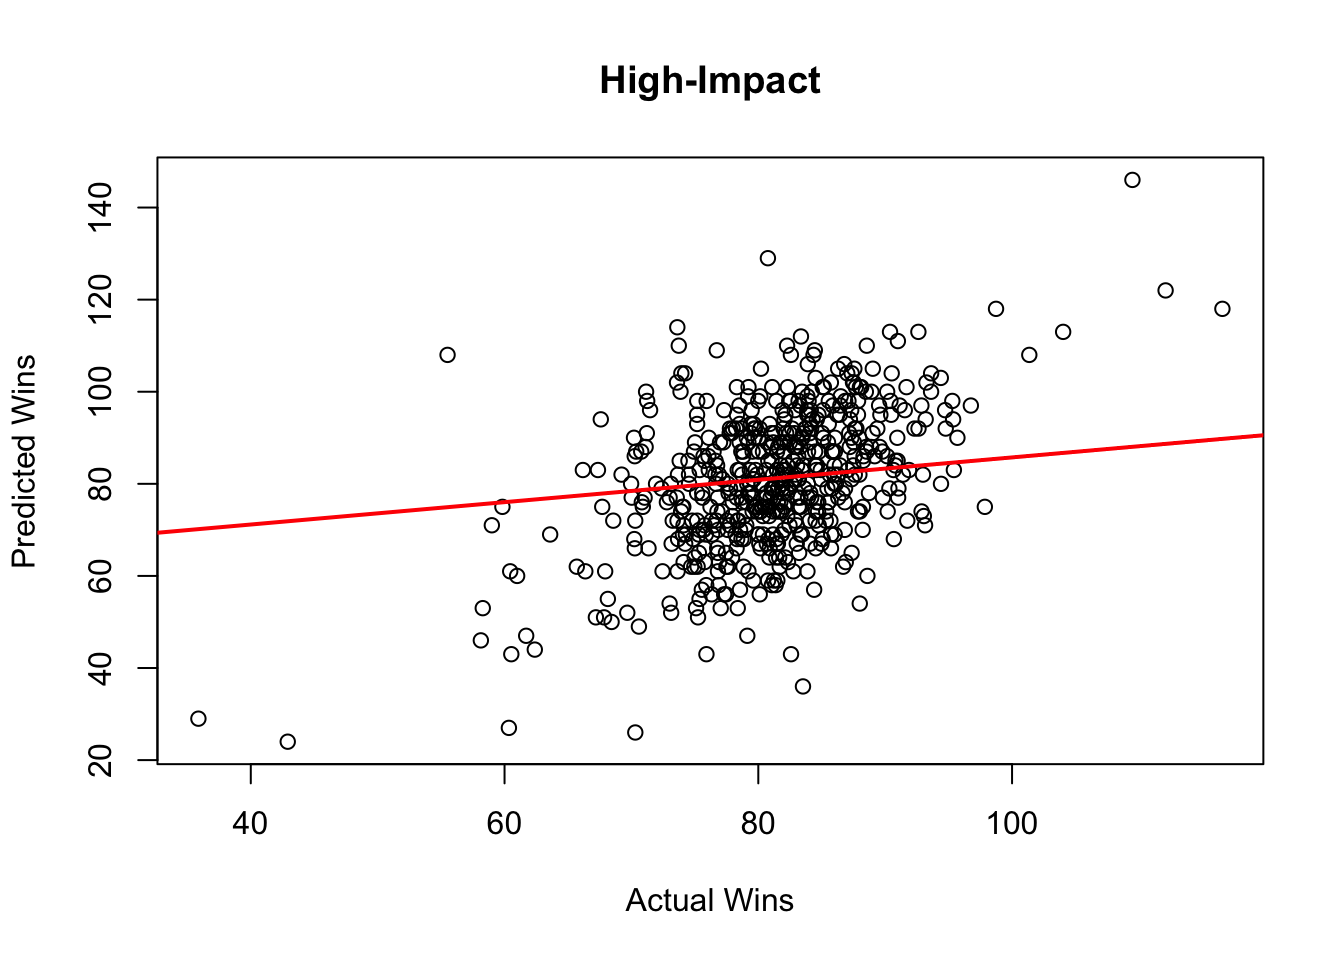
\includegraphics{Assignment1_Data621_HW_files/figure-latex/unnamed-chunk-44-1.pdf}

Our diagnostic plots show a fairly linear model.

Normality

\begin{Shaded}
\begin{Highlighting}[]
\FunctionTok{plot}\NormalTok{(log\_model1, }\AttributeTok{which=}\DecValTok{2}\NormalTok{)}
\end{Highlighting}
\end{Shaded}

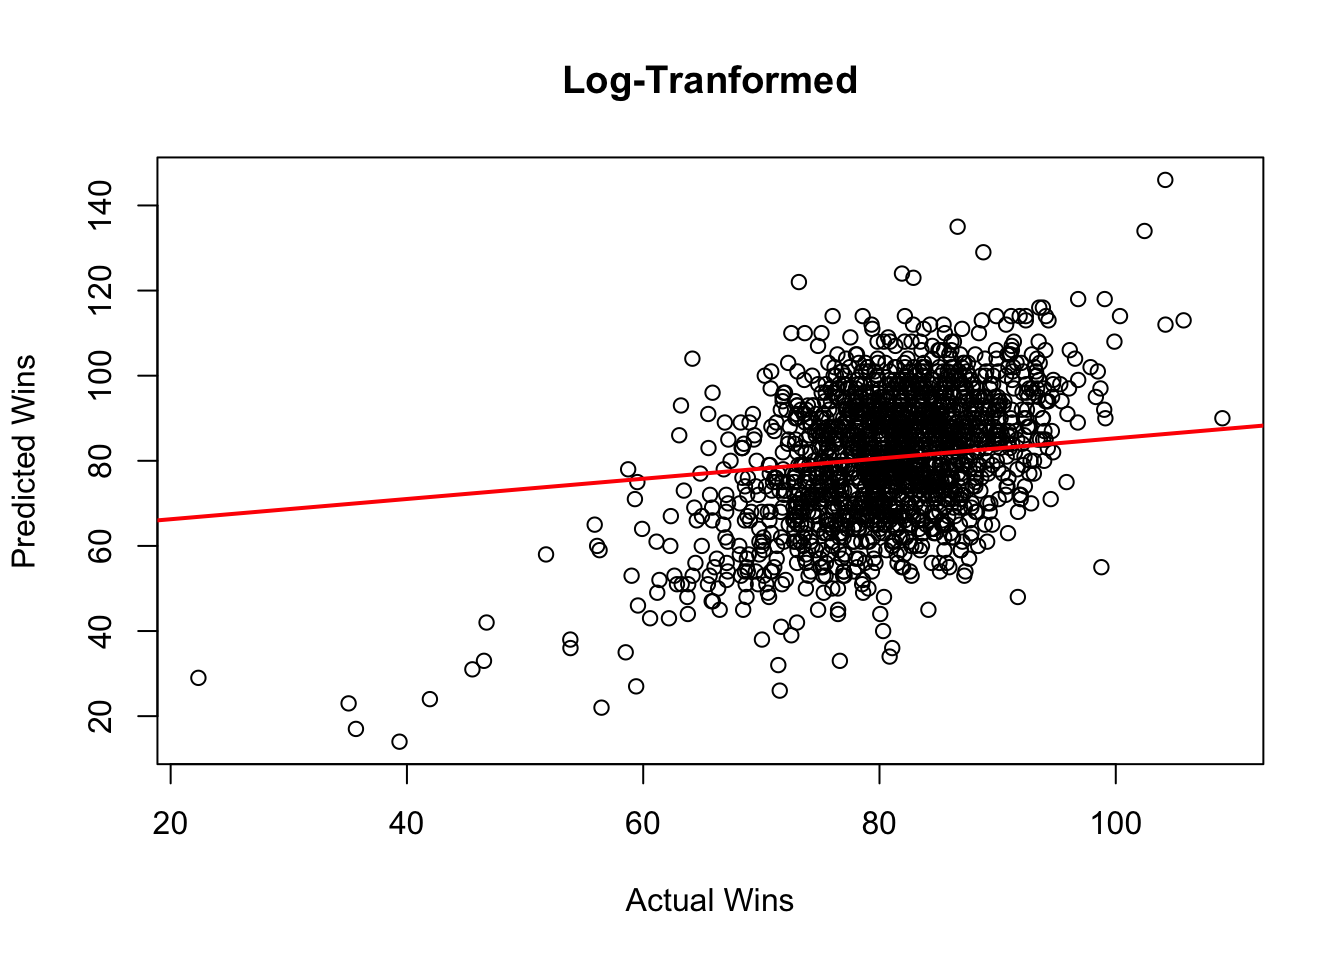
\includegraphics{Assignment1_Data621_HW_files/figure-latex/unnamed-chunk-45-1.pdf}

\begin{Shaded}
\begin{Highlighting}[]
\FunctionTok{shapiro.test}\NormalTok{(}\FunctionTok{residuals}\NormalTok{(log\_model1))}
\end{Highlighting}
\end{Shaded}

\begin{verbatim}
## 
##  Shapiro-Wilk normality test
## 
## data:  residuals(log_model1)
## W = 0.99862, p-value = 0.1927
\end{verbatim}

\begin{Shaded}
\begin{Highlighting}[]
\CommentTok{\# Shapiro{-}Wilk normality test: look for high p{-}value}
\end{Highlighting}
\end{Shaded}

Our QQ plot suggests normality thought there is obvious skewing on the
tails, particularly on the right. A Shapiro Wilk's Test statistic
restulted in a value of 0.9986 suggesting normality.

Heteroscedasticity:

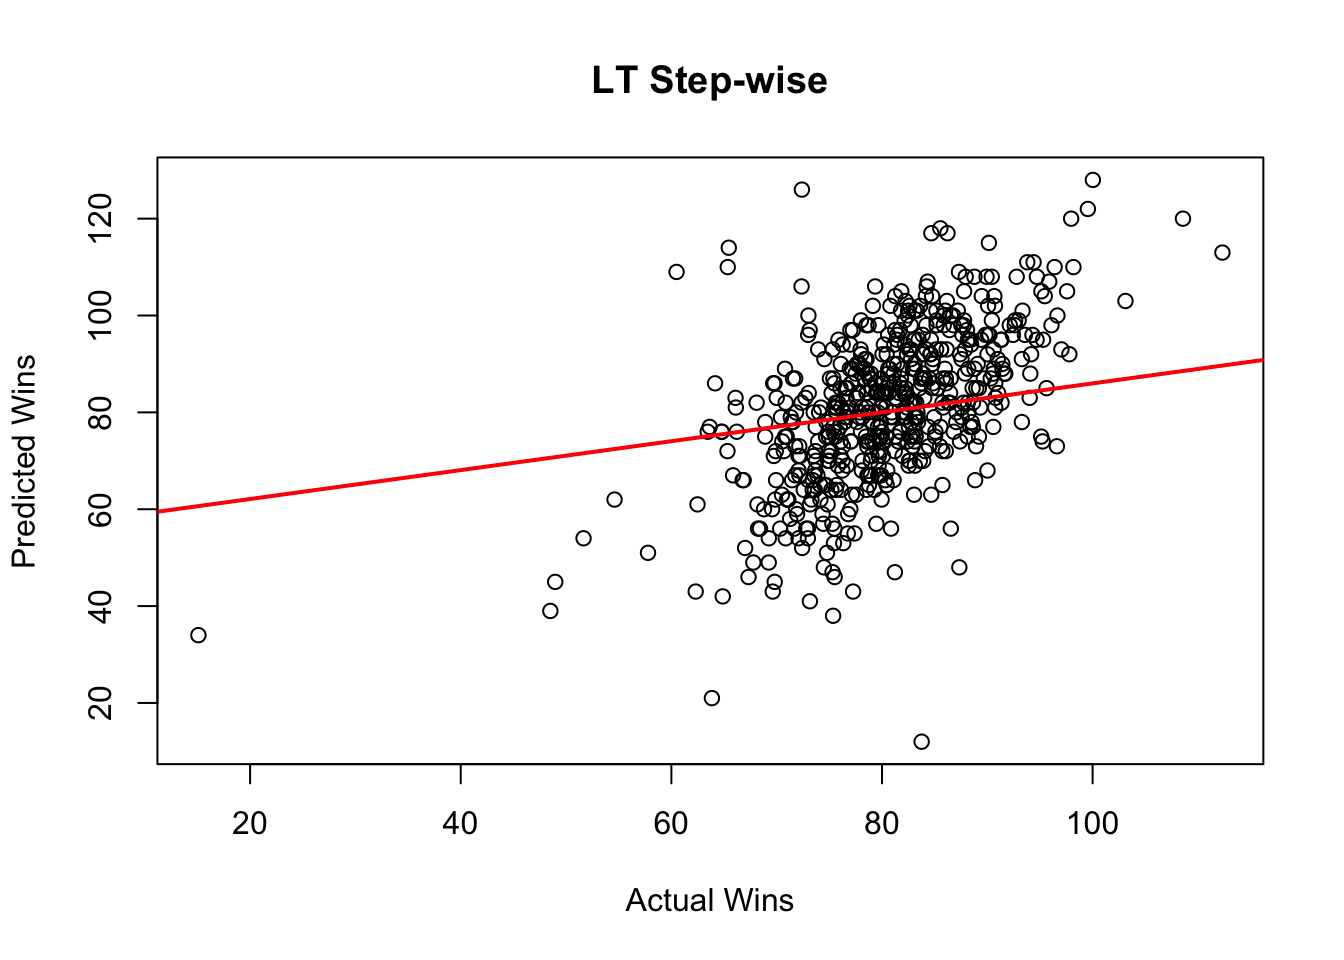
\includegraphics{Assignment1_Data621_HW_files/figure-latex/unnamed-chunk-46-1.pdf}
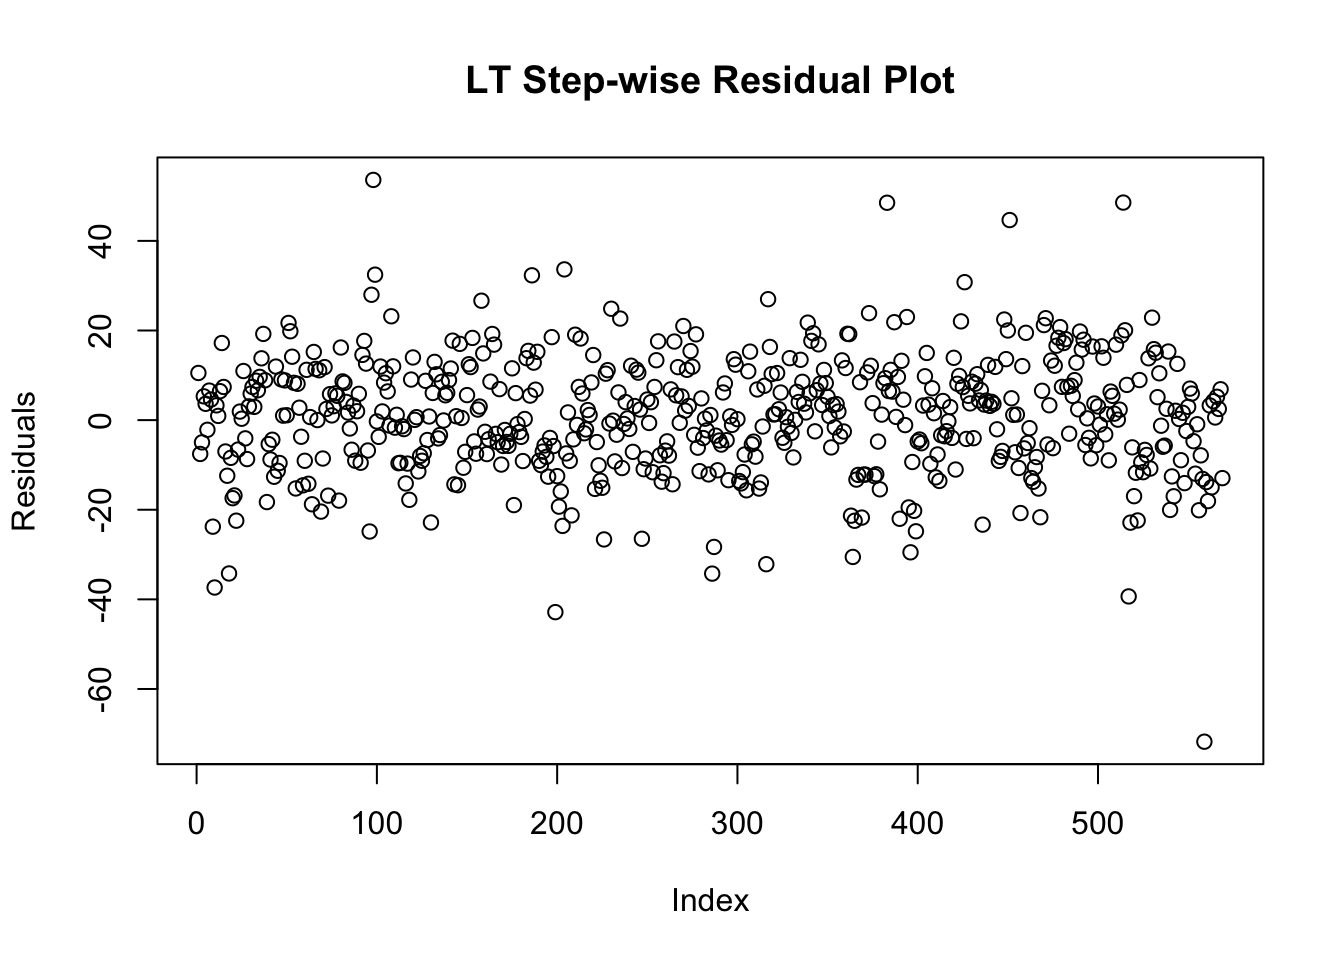
\includegraphics{Assignment1_Data621_HW_files/figure-latex/unnamed-chunk-46-2.pdf}

\begin{verbatim}
## 
##  studentized Breusch-Pagan test
## 
## data:  log_model1
## BP = 152.45, df = 4, p-value < 2.2e-16
\end{verbatim}

Our Scale-Location plot shows no major improvement than our previous
models. While the points appear somewhat evenly distributed above and
below the trend line and there is no obvious fan/wedge pattern, there is
clustering in the center suggesting underfitting, high leverage outliers
or that additional transformation may be needed. As our Cook's Distance
plot has no values with a greater than 1, we can rule our the effects of
high leverage points.

The Breusch-Page test statistic BP (152.45) and the small p-value
(2.2e-16) suggest evidence of heteroscedasticity. Though the values are
different that we may need to transform the data to meet the Assumption
of Homoscedasticity.

Independence:

\begin{Shaded}
\begin{Highlighting}[]
\FunctionTok{acf}\NormalTok{(}\FunctionTok{residuals}\NormalTok{(log\_model1))}
\end{Highlighting}
\end{Shaded}

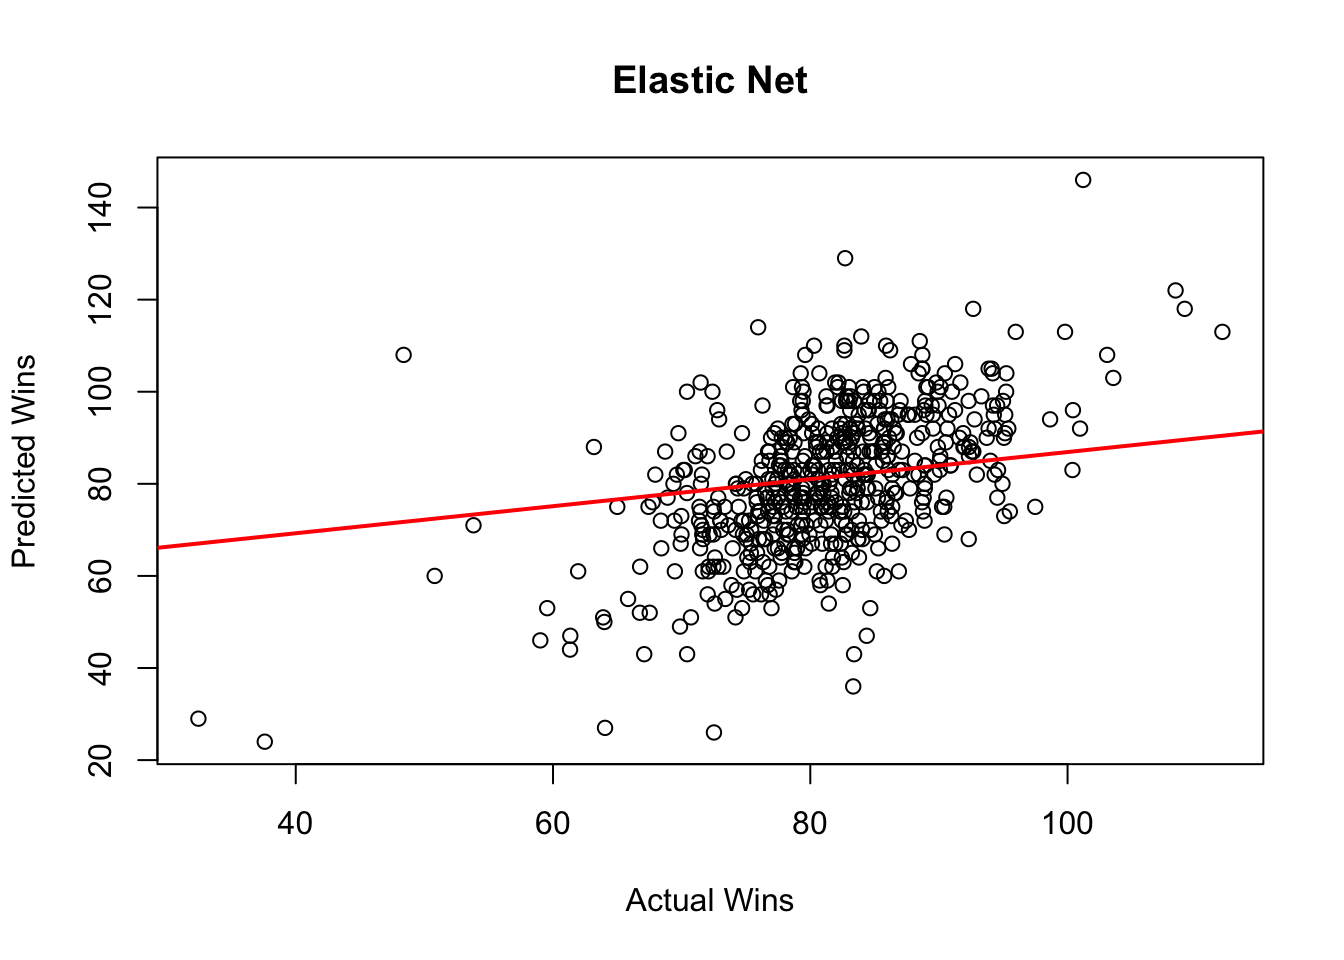
\includegraphics{Assignment1_Data621_HW_files/figure-latex/unnamed-chunk-47-1.pdf}

\begin{Shaded}
\begin{Highlighting}[]
\FunctionTok{durbinWatsonTest}\NormalTok{(log\_model1)}
\end{Highlighting}
\end{Shaded}

\begin{verbatim}
##  lag Autocorrelation D-W Statistic p-value
##    1     0.004317842      1.990818   0.812
##  Alternative hypothesis: rho != 0
\end{verbatim}

\begin{Shaded}
\begin{Highlighting}[]
\CommentTok{\# Durbin Watson should be close to 2}
\end{Highlighting}
\end{Shaded}

Our Autocorrelation Function and Durbin-Watson test suggest that our
model's residuals are independent and therefore do not violate the
Independence Assumption.

\paragraph{Model T2: Applying Log Transformation to Key
Predictors}\label{model-t2-applying-log-transformation-to-key-predictors}

Below is a variation of the above with some minor adjustments that
exclude log\_PITCHING\_SO and include TEAM\_BASERUN\_SB.

\begin{Shaded}
\begin{Highlighting}[]
\CommentTok{\# Transformation applied to account for skewed distributions in key predictors}

\NormalTok{target\_vars3 }\OtherTok{\textless{}{-}} \FunctionTok{c}\NormalTok{(}\StringTok{"log\_TEAM\_BATTING\_H"}\NormalTok{, }\StringTok{"log\_TEAM\_BATTING\_HR"}\NormalTok{, }\StringTok{"TEAM\_BATTING\_BB"}\NormalTok{, }\StringTok{"TEAM\_BASERUN\_SB"}\NormalTok{, }\StringTok{"TEAM\_FIELDING\_E"}\NormalTok{)}
\NormalTok{log\_model2 }\OtherTok{\textless{}{-}} \FunctionTok{lm}\NormalTok{(TARGET\_WINS }\SpecialCharTok{\textasciitilde{}}\NormalTok{ ., }\AttributeTok{data =}\NormalTok{ train\_df\_log[, }\FunctionTok{c}\NormalTok{(}\StringTok{"TARGET\_WINS"}\NormalTok{, target\_vars3)])}
\FunctionTok{summary}\NormalTok{(log\_model2)}
\end{Highlighting}
\end{Shaded}

\begin{verbatim}
## 
## Call:
## lm(formula = TARGET_WINS ~ ., data = train_df_log[, c("TARGET_WINS", 
##     target_vars3)])
## 
## Residuals:
##     Min      1Q  Median      3Q     Max 
## -52.560  -8.851  -0.049   8.855  52.489 
## 
## Coefficients:
##                       Estimate Std. Error t value Pr(>|t|)    
## (Intercept)         -4.867e+02  2.681e+01 -18.153  < 2e-16 ***
## log_TEAM_BATTING_H   7.771e+01  3.794e+00  20.480  < 2e-16 ***
## log_TEAM_BATTING_HR -4.234e-01  5.819e-01  -0.728   0.4670    
## TEAM_BATTING_BB      7.382e-03  3.887e-03   1.899   0.0577 .  
## TEAM_BASERUN_SB      3.488e-02  4.419e-03   7.893 5.23e-15 ***
## TEAM_FIELDING_E     -2.113e-02  2.372e-03  -8.909  < 2e-16 ***
## ---
## Signif. codes:  0 '***' 0.001 '**' 0.01 '*' 0.05 '.' 0.1 ' ' 1
## 
## Residual standard error: 13.49 on 1696 degrees of freedom
## Multiple R-squared:  0.2636, Adjusted R-squared:  0.2614 
## F-statistic: 121.4 on 5 and 1696 DF,  p-value: < 2.2e-16
\end{verbatim}

\subparagraph{Model Diagnostics}\label{model-diagnostics-1}

Our VIF Test and diagnostic plots show similar results as the
diagnostics for Model T1.

\begin{Shaded}
\begin{Highlighting}[]
\FunctionTok{vif}\NormalTok{(log\_model2)}
\end{Highlighting}
\end{Shaded}

\begin{verbatim}
##  log_TEAM_BATTING_H log_TEAM_BATTING_HR     TEAM_BATTING_BB     TEAM_BASERUN_SB 
##            1.172671            2.238759            2.078787            1.363852 
##     TEAM_FIELDING_E 
##            2.589296
\end{verbatim}

\begin{Shaded}
\begin{Highlighting}[]
\FunctionTok{plot}\NormalTok{(log\_model2)}
\end{Highlighting}
\end{Shaded}

\includegraphics{Assignment1_Data621_HW_files/figure-latex/unnamed-chunk-49-1.pdf}
\includegraphics{Assignment1_Data621_HW_files/figure-latex/unnamed-chunk-49-2.pdf}
\includegraphics{Assignment1_Data621_HW_files/figure-latex/unnamed-chunk-49-3.pdf}
\includegraphics{Assignment1_Data621_HW_files/figure-latex/unnamed-chunk-49-4.pdf}

Our diagnostic plots show a fairly linear model.

\paragraph{Model T3: Log Transformation on the Dependent Variable
(Y)}\label{model-t3-log-transformation-on-the-dependent-variable-y}

\begin{Shaded}
\begin{Highlighting}[]
\NormalTok{stp\_logy\_model }\OtherTok{\textless{}{-}} \FunctionTok{lm}\NormalTok{(}\FunctionTok{log}\NormalTok{(TARGET\_WINS }\SpecialCharTok{+} \DecValTok{1}\NormalTok{) }\SpecialCharTok{\textasciitilde{}}\NormalTok{., }\AttributeTok{data =}\NormalTok{ stp75\_train\_df)}

\CommentTok{\# Backward step{-}wise regression}
\NormalTok{stpb\_logy\_model }\OtherTok{\textless{}{-}} \FunctionTok{step}\NormalTok{(stp\_logy\_model, }\AttributeTok{direction =} \StringTok{"backward"}\NormalTok{)}
\end{Highlighting}
\end{Shaded}

\begin{verbatim}
## Start:  AIC=-5905.5
## log(TARGET_WINS + 1) ~ TEAM_BATTING_H + TEAM_BATTING_2B + TEAM_BATTING_3B + 
##     TEAM_BATTING_HR + TEAM_BATTING_BB + TEAM_BATTING_SO + TEAM_BASERUN_SB + 
##     TEAM_BASERUN_CS + TEAM_PITCHING_H + TEAM_PITCHING_HR + TEAM_PITCHING_BB + 
##     TEAM_PITCHING_SO + TEAM_FIELDING_E + TEAM_FIELDING_DP
## 
##                    Df Sum of Sq    RSS     AIC
## - TEAM_BATTING_HR   1    0.0017 52.051 -5907.4
## - TEAM_PITCHING_BB  1    0.0034 52.053 -5907.4
## - TEAM_PITCHING_SO  1    0.0039 52.053 -5907.4
## - TEAM_BATTING_SO   1    0.0077 52.057 -5907.3
## - TEAM_BASERUN_CS   1    0.0112 52.060 -5907.1
## - TEAM_BATTING_BB   1    0.0165 52.066 -5907.0
## - TEAM_PITCHING_HR  1    0.0468 52.096 -5906.0
## <none>                          52.049 -5905.5
## - TEAM_BATTING_2B   1    0.0885 52.138 -5904.6
## - TEAM_PITCHING_H   1    0.2636 52.313 -5898.9
## - TEAM_BATTING_3B   1    0.4776 52.527 -5892.0
## - TEAM_BASERUN_SB   1    0.9296 52.979 -5877.4
## - TEAM_FIELDING_DP  1    1.7237 53.773 -5852.0
## - TEAM_FIELDING_E   1    2.1095 54.159 -5839.9
## - TEAM_BATTING_H    1    3.8849 55.934 -5785.0
## 
## Step:  AIC=-5907.45
## log(TARGET_WINS + 1) ~ TEAM_BATTING_H + TEAM_BATTING_2B + TEAM_BATTING_3B + 
##     TEAM_BATTING_BB + TEAM_BATTING_SO + TEAM_BASERUN_SB + TEAM_BASERUN_CS + 
##     TEAM_PITCHING_H + TEAM_PITCHING_HR + TEAM_PITCHING_BB + TEAM_PITCHING_SO + 
##     TEAM_FIELDING_E + TEAM_FIELDING_DP
## 
##                    Df Sum of Sq    RSS     AIC
## - TEAM_PITCHING_BB  1    0.0021 52.053 -5909.4
## - TEAM_PITCHING_SO  1    0.0033 52.054 -5909.3
## - TEAM_BATTING_SO   1    0.0064 52.057 -5909.2
## - TEAM_BASERUN_CS   1    0.0122 52.063 -5909.0
## - TEAM_BATTING_BB   1    0.0228 52.074 -5908.7
## <none>                          52.051 -5907.4
## - TEAM_BATTING_2B   1    0.0903 52.141 -5906.5
## - TEAM_PITCHING_H   1    0.3306 52.382 -5898.7
## - TEAM_BATTING_3B   1    0.4849 52.536 -5893.7
## - TEAM_PITCHING_HR  1    0.7126 52.764 -5886.3
## - TEAM_BASERUN_SB   1    0.9292 52.980 -5879.3
## - TEAM_FIELDING_DP  1    1.7221 53.773 -5854.0
## - TEAM_FIELDING_E   1    2.1146 54.166 -5841.7
## - TEAM_BATTING_H    1    4.0738 56.125 -5781.2
## 
## Step:  AIC=-5909.38
## log(TARGET_WINS + 1) ~ TEAM_BATTING_H + TEAM_BATTING_2B + TEAM_BATTING_3B + 
##     TEAM_BATTING_BB + TEAM_BATTING_SO + TEAM_BASERUN_SB + TEAM_BASERUN_CS + 
##     TEAM_PITCHING_H + TEAM_PITCHING_HR + TEAM_PITCHING_SO + TEAM_FIELDING_E + 
##     TEAM_FIELDING_DP
## 
##                    Df Sum of Sq    RSS     AIC
## - TEAM_PITCHING_SO  1    0.0104 52.064 -5911.0
## - TEAM_BASERUN_CS   1    0.0125 52.066 -5911.0
## - TEAM_BATTING_SO   1    0.0137 52.067 -5910.9
## <none>                          52.053 -5909.4
## - TEAM_BATTING_2B   1    0.0901 52.143 -5908.4
## - TEAM_BATTING_BB   1    0.1039 52.157 -5908.0
## - TEAM_PITCHING_H   1    0.4160 52.469 -5897.8
## - TEAM_BATTING_3B   1    0.4965 52.550 -5895.2
## - TEAM_PITCHING_HR  1    0.7393 52.792 -5887.4
## - TEAM_BASERUN_SB   1    1.0027 53.056 -5878.9
## - TEAM_FIELDING_DP  1    1.7211 53.774 -5856.0
## - TEAM_FIELDING_E   1    2.1317 54.185 -5843.1
## - TEAM_BATTING_H    1    4.1341 56.187 -5781.3
## 
## Step:  AIC=-5911.04
## log(TARGET_WINS + 1) ~ TEAM_BATTING_H + TEAM_BATTING_2B + TEAM_BATTING_3B + 
##     TEAM_BATTING_BB + TEAM_BATTING_SO + TEAM_BASERUN_SB + TEAM_BASERUN_CS + 
##     TEAM_PITCHING_H + TEAM_PITCHING_HR + TEAM_FIELDING_E + TEAM_FIELDING_DP
## 
##                    Df Sum of Sq    RSS     AIC
## - TEAM_BATTING_SO   1    0.0045 52.068 -5912.9
## - TEAM_BASERUN_CS   1    0.0117 52.075 -5912.7
## <none>                          52.064 -5911.0
## - TEAM_BATTING_2B   1    0.0850 52.149 -5910.3
## - TEAM_BATTING_BB   1    0.1013 52.165 -5909.7
## - TEAM_PITCHING_H   1    0.4113 52.475 -5899.6
## - TEAM_BATTING_3B   1    0.5197 52.583 -5896.1
## - TEAM_PITCHING_HR  1    0.7525 52.816 -5888.6
## - TEAM_BASERUN_SB   1    0.9956 53.059 -5880.8
## - TEAM_FIELDING_DP  1    1.7162 53.780 -5857.8
## - TEAM_FIELDING_E   1    2.2464 54.310 -5841.1
## - TEAM_BATTING_H    1    4.2185 56.282 -5780.4
## 
## Step:  AIC=-5912.89
## log(TARGET_WINS + 1) ~ TEAM_BATTING_H + TEAM_BATTING_2B + TEAM_BATTING_3B + 
##     TEAM_BATTING_BB + TEAM_BASERUN_SB + TEAM_BASERUN_CS + TEAM_PITCHING_H + 
##     TEAM_PITCHING_HR + TEAM_FIELDING_E + TEAM_FIELDING_DP
## 
##                    Df Sum of Sq    RSS     AIC
## - TEAM_BASERUN_CS   1    0.0119 52.080 -5914.5
## <none>                          52.068 -5912.9
## - TEAM_BATTING_2B   1    0.1060 52.174 -5911.4
## - TEAM_BATTING_BB   1    0.1130 52.181 -5911.2
## - TEAM_PITCHING_H   1    0.4112 52.479 -5901.5
## - TEAM_BATTING_3B   1    0.5809 52.649 -5896.0
## - TEAM_PITCHING_HR  1    1.0350 53.103 -5881.4
## - TEAM_BASERUN_SB   1    1.0365 53.104 -5881.3
## - TEAM_FIELDING_DP  1    1.7139 53.782 -5859.8
## - TEAM_FIELDING_E   1    2.2461 54.314 -5843.0
## - TEAM_BATTING_H    1    5.9379 58.006 -5731.1
## 
## Step:  AIC=-5914.5
## log(TARGET_WINS + 1) ~ TEAM_BATTING_H + TEAM_BATTING_2B + TEAM_BATTING_3B + 
##     TEAM_BATTING_BB + TEAM_BASERUN_SB + TEAM_PITCHING_H + TEAM_PITCHING_HR + 
##     TEAM_FIELDING_E + TEAM_FIELDING_DP
## 
##                    Df Sum of Sq    RSS     AIC
## <none>                          52.080 -5914.5
## - TEAM_BATTING_2B   1    0.1092 52.189 -5912.9
## - TEAM_BATTING_BB   1    0.1217 52.202 -5912.5
## - TEAM_PITCHING_H   1    0.4353 52.515 -5902.3
## - TEAM_BATTING_3B   1    0.5855 52.665 -5897.5
## - TEAM_BASERUN_SB   1    1.0369 53.117 -5882.9
## - TEAM_PITCHING_HR  1    1.1443 53.224 -5879.5
## - TEAM_FIELDING_DP  1    1.7267 53.807 -5861.0
## - TEAM_FIELDING_E   1    2.2913 54.371 -5843.2
## - TEAM_BATTING_H    1    5.9315 58.011 -5732.9
\end{verbatim}

\subparagraph{Diagnosing our Model}\label{diagnosing-our-model-2}

Linearity

\begin{Shaded}
\begin{Highlighting}[]
\FunctionTok{plot}\NormalTok{(stp\_logy\_model, }\AttributeTok{which=}\DecValTok{1}\NormalTok{)}
\end{Highlighting}
\end{Shaded}

\includegraphics{Assignment1_Data621_HW_files/figure-latex/unnamed-chunk-50-1.pdf}

Our Residuals vs.~Fitted plot suggests a somewhat linear model but there
is visible bowing in the trend line.

Normality

\begin{Shaded}
\begin{Highlighting}[]
\FunctionTok{plot}\NormalTok{(stp\_logy\_model, }\AttributeTok{which =} \DecValTok{2}\NormalTok{)}
\end{Highlighting}
\end{Shaded}

\includegraphics{Assignment1_Data621_HW_files/figure-latex/unnamed-chunk-51-1.pdf}

\begin{Shaded}
\begin{Highlighting}[]
\FunctionTok{shapiro.test}\NormalTok{(}\FunctionTok{residuals}\NormalTok{(stp\_logy\_model))}
\end{Highlighting}
\end{Shaded}

\begin{verbatim}
## 
##  Shapiro-Wilk normality test
## 
## data:  residuals(stp_logy_model)
## W = 0.9762, p-value = 3.367e-16
\end{verbatim}

\begin{Shaded}
\begin{Highlighting}[]
\CommentTok{\# Shapiro{-}Wilk normality test: look for high p{-}value}
\end{Highlighting}
\end{Shaded}

Our QQ plot suggests normality thought there is obvious skewing on the
tails, particularly on the left.

A Shapiro Wilk's Test statistic had a value of 0.980, also suggesting
normality. However, since the p-value (1.416e-14) is less than
\textless{} 0.05 we may still be violating our normality assumption.

Heteroscedasticity

\includegraphics{Assignment1_Data621_HW_files/figure-latex/unnamed-chunk-52-1.pdf}
\includegraphics{Assignment1_Data621_HW_files/figure-latex/unnamed-chunk-52-2.pdf}

\begin{verbatim}
## 
##  studentized Breusch-Pagan test
## 
## data:  stp_logy_model
## BP = 270.46, df = 14, p-value < 2.2e-16
\end{verbatim}

Our Scale-Location plot shows clear bowing in the trend line, suggesting
that the variance of the residuals is not constant and therefore
heteroschedastic. While there is no obvious fan/wedge pattern, there is
clustering in the center suggesting underfitting, high leverage outliers
or that additional transformation may be needed. As our Cook's Distance
plot has no values with a greater than 1, we can rule our the effects of
high leverage points. However, it should be pointed the leverage points
appear to be more influential than in our backwards selected model or
our Box-Cox transformed model.

The Breusch-Page test statistic BP (383.07) indicates a substantial
relationship between the residual variance and the predictors and the
small p-value (2.2e-16) suggest evidence of heteroscedasticity. Though
the values are different that we may need to transform the data to meet
the Assumption of Homoscedasticity.

Independence

\begin{Shaded}
\begin{Highlighting}[]
\FunctionTok{acf}\NormalTok{(}\FunctionTok{residuals}\NormalTok{(stp\_logy\_model))}
\end{Highlighting}
\end{Shaded}

\includegraphics{Assignment1_Data621_HW_files/figure-latex/unnamed-chunk-53-1.pdf}

\begin{Shaded}
\begin{Highlighting}[]
\FunctionTok{durbinWatsonTest}\NormalTok{(stp\_logy\_model)}
\end{Highlighting}
\end{Shaded}

\begin{verbatim}
##  lag Autocorrelation D-W Statistic p-value
##    1     -0.01440497      2.028171   0.582
##  Alternative hypothesis: rho != 0
\end{verbatim}

\begin{Shaded}
\begin{Highlighting}[]
\CommentTok{\# Durbin Watson should be close to 2}
\end{Highlighting}
\end{Shaded}

Our Autocorrelation Function shows that there are lags above the blue
dashed line, suggesting no autocorrelation. This is confirmed through a
Durbin-Watson test statistic value of 2.00 and an autocorrelation value
of -0.0041. Furthermore, as our p-value (0.96) is greater than 0.05, we
do not have enough evidence to reject the null hypothesis that there is
no autocorrelation. In other words, the test results suggest that our
model's residuals are independent and therefore do not violate the
Independence Assumption.

\emph{Conclusion} Applying a log transformation the dependent variable
in our model appears to inferior to the backward selected model and the
Box-Cox transformed model. We should therefore avoid using this model.

\paragraph{Model T4: Log Transformation on Independent Variables
(X)}\label{model-t4-log-transformation-on-independent-variables-x}

Some of our predictors (TEAM\_PITCHING\_SO, TEAM\_PITCHING\_BB, \&
TEAM\_PITCHING\_H) showed the presence of outliers. We will transform
these variables with a log transformation.

\subparagraph{Backwards Selection}\label{backwards-selection}

We will use backward step-wise selection to build our model.

\begin{Shaded}
\begin{Highlighting}[]
\NormalTok{stp\_logx\_model\_full }\OtherTok{\textless{}{-}} \FunctionTok{lm}\NormalTok{(TARGET\_WINS }\SpecialCharTok{\textasciitilde{}}\NormalTok{ . }\SpecialCharTok{{-}}\NormalTok{ TEAM\_BATTING\_H }\SpecialCharTok{{-}}\NormalTok{ TEAM\_BATTING\_HR }\SpecialCharTok{{-}}\NormalTok{ TEAM\_PITCHING\_SO }\SpecialCharTok{{-}}\NormalTok{ TEAM\_PITCHING\_BB, }\AttributeTok{data =}\NormalTok{ train\_df\_log)}

\CommentTok{\# Backward step{-}wise regression}
\NormalTok{stp\_logx\_model }\OtherTok{\textless{}{-}} \FunctionTok{step}\NormalTok{(stp\_logx\_model\_full, }\AttributeTok{direction =} \StringTok{"backward"}\NormalTok{)}
\end{Highlighting}
\end{Shaded}

\begin{verbatim}
## Start:  AIC=8743.2
## TARGET_WINS ~ (TEAM_BATTING_H + TEAM_BATTING_2B + TEAM_BATTING_3B + 
##     TEAM_BATTING_HR + TEAM_BATTING_BB + TEAM_BATTING_SO + TEAM_BASERUN_SB + 
##     TEAM_BASERUN_CS + TEAM_PITCHING_H + TEAM_PITCHING_HR + TEAM_PITCHING_BB + 
##     TEAM_PITCHING_SO + TEAM_FIELDING_E + TEAM_FIELDING_DP + log_TEAM_BATTING_H + 
##     log_TEAM_BATTING_HR + log_TEAM_PITCHING_SO + log_TEAM_PITCHING_BB) - 
##     TEAM_BATTING_H - TEAM_BATTING_HR - TEAM_PITCHING_SO - TEAM_PITCHING_BB
## 
##                        Df Sum of Sq    RSS    AIC
## - TEAM_PITCHING_H       1      26.4 284658 8741.4
## - TEAM_BASERUN_CS       1     170.2 284801 8742.2
## <none>                              284631 8743.2
## - TEAM_BATTING_2B       1     396.4 285028 8743.6
## - log_TEAM_BATTING_HR   1    1218.3 285849 8748.5
## - TEAM_BATTING_3B       1    3580.3 288211 8762.5
## - TEAM_BATTING_SO       1    3726.0 288357 8763.3
## - log_TEAM_PITCHING_SO  1    4182.4 288814 8766.0
## - log_TEAM_PITCHING_BB  1    4656.5 289288 8768.8
## - TEAM_PITCHING_HR      1    4673.5 289305 8768.9
## - TEAM_BATTING_BB       1    5801.7 290433 8775.5
## - TEAM_FIELDING_DP      1    6585.0 291216 8780.1
## - TEAM_BASERUN_SB       1    6984.5 291616 8782.5
## - TEAM_FIELDING_E       1   11106.8 295738 8806.4
## - log_TEAM_BATTING_H    1   21311.0 305942 8864.1
## 
## Step:  AIC=8741.36
## TARGET_WINS ~ TEAM_BATTING_2B + TEAM_BATTING_3B + TEAM_BATTING_BB + 
##     TEAM_BATTING_SO + TEAM_BASERUN_SB + TEAM_BASERUN_CS + TEAM_PITCHING_HR + 
##     TEAM_FIELDING_E + TEAM_FIELDING_DP + log_TEAM_BATTING_H + 
##     log_TEAM_BATTING_HR + log_TEAM_PITCHING_SO + log_TEAM_PITCHING_BB
## 
##                        Df Sum of Sq    RSS    AIC
## - TEAM_BASERUN_CS       1     186.1 284844 8740.5
## <none>                              284658 8741.4
## - TEAM_BATTING_2B       1     388.8 285046 8741.7
## - log_TEAM_BATTING_HR   1    1196.6 285854 8746.5
## - TEAM_BATTING_SO       1    3761.9 288420 8761.7
## - TEAM_BATTING_3B       1    3893.4 288551 8762.5
## - log_TEAM_PITCHING_SO  1    4354.1 289012 8765.2
## - TEAM_PITCHING_HR      1    4754.0 289412 8767.5
## - TEAM_FIELDING_DP      1    6560.5 291218 8778.1
## - log_TEAM_PITCHING_BB  1    6889.6 291547 8780.1
## - TEAM_BASERUN_SB       1    7323.2 291981 8782.6
## - TEAM_BATTING_BB       1    8126.4 292784 8787.3
## - TEAM_FIELDING_E       1   13833.0 298491 8820.1
## - log_TEAM_BATTING_H    1   21625.3 306283 8864.0
## 
## Step:  AIC=8740.47
## TARGET_WINS ~ TEAM_BATTING_2B + TEAM_BATTING_3B + TEAM_BATTING_BB + 
##     TEAM_BATTING_SO + TEAM_BASERUN_SB + TEAM_PITCHING_HR + TEAM_FIELDING_E + 
##     TEAM_FIELDING_DP + log_TEAM_BATTING_H + log_TEAM_BATTING_HR + 
##     log_TEAM_PITCHING_SO + log_TEAM_PITCHING_BB
## 
##                        Df Sum of Sq    RSS    AIC
## <none>                              284844 8740.5
## - TEAM_BATTING_2B       1     406.4 285250 8740.9
## - log_TEAM_BATTING_HR   1    1192.6 286036 8745.6
## - TEAM_BATTING_SO       1    3760.6 288604 8760.8
## - TEAM_BATTING_3B       1    3975.0 288819 8762.1
## - log_TEAM_PITCHING_SO  1    4354.3 289198 8764.3
## - TEAM_PITCHING_HR      1    5012.9 289857 8768.2
## - TEAM_FIELDING_DP      1    6635.4 291479 8777.7
## - log_TEAM_PITCHING_BB  1    7046.7 291890 8780.1
## - TEAM_BASERUN_SB       1    7142.4 291986 8780.6
## - TEAM_BATTING_BB       1    8481.9 293326 8788.4
## - TEAM_FIELDING_E       1   13710.7 298554 8818.5
## - log_TEAM_BATTING_H    1   21510.4 306354 8862.4
\end{verbatim}

Looking at the summary for this model shows that all predictors have
high statistic significance.

\begin{Shaded}
\begin{Highlighting}[]
\FunctionTok{summary}\NormalTok{(stp\_logx\_model)}
\end{Highlighting}
\end{Shaded}

\begin{verbatim}
## 
## Call:
## lm(formula = TARGET_WINS ~ TEAM_BATTING_2B + TEAM_BATTING_3B + 
##     TEAM_BATTING_BB + TEAM_BATTING_SO + TEAM_BASERUN_SB + TEAM_PITCHING_HR + 
##     TEAM_FIELDING_E + TEAM_FIELDING_DP + log_TEAM_BATTING_H + 
##     log_TEAM_BATTING_HR + log_TEAM_PITCHING_SO + log_TEAM_PITCHING_BB, 
##     data = train_df_log)
## 
## Residuals:
##     Min      1Q  Median      3Q     Max 
## -46.947  -8.180  -0.139   8.503  57.195 
## 
## Coefficients:
##                        Estimate Std. Error t value Pr(>|t|)    
## (Intercept)          -4.665e+02  5.633e+01  -8.281 2.45e-16 ***
## TEAM_BATTING_2B      -1.678e-02  1.081e-02  -1.552  0.12075    
## TEAM_BATTING_3B       9.285e-02  1.913e-02   4.855 1.32e-06 ***
## TEAM_BATTING_BB       5.165e-02  7.283e-03   7.092 1.94e-12 ***
## TEAM_BATTING_SO      -2.377e-02  5.033e-03  -4.722 2.53e-06 ***
## TEAM_BASERUN_SB       3.123e-02  4.799e-03   6.508 1.00e-10 ***
## TEAM_PITCHING_HR      8.489e-02  1.557e-02   5.452 5.72e-08 ***
## TEAM_FIELDING_E      -2.582e-02  2.863e-03  -9.017  < 2e-16 ***
## TEAM_FIELDING_DP     -9.686e-02  1.544e-02  -6.273 4.50e-10 ***
## log_TEAM_BATTING_H    7.897e+01  6.992e+00  11.294  < 2e-16 ***
## log_TEAM_BATTING_HR  -3.269e+00  1.229e+00  -2.659  0.00791 ** 
## log_TEAM_PITCHING_SO  1.634e+01  3.216e+00   5.081 4.17e-07 ***
## log_TEAM_PITCHING_BB -1.984e+01  3.070e+00  -6.464 1.33e-10 ***
## ---
## Signif. codes:  0 '***' 0.001 '**' 0.01 '*' 0.05 '.' 0.1 ' ' 1
## 
## Residual standard error: 12.99 on 1689 degrees of freedom
## Multiple R-squared:  0.3206, Adjusted R-squared:  0.3158 
## F-statistic: 66.43 on 12 and 1689 DF,  p-value: < 2.2e-16
\end{verbatim}

The Residuals vs.~Fitted and QQ Plots show a fairly linear pattern,
while Scale-Location plot suggest Homoscedasticity. The Residuals vs
Leverage plot reveals that our outliers have less leverage than in the
pre- log transformed model.

\begin{Shaded}
\begin{Highlighting}[]
\FunctionTok{plot}\NormalTok{(stp\_logx\_model)}
\end{Highlighting}
\end{Shaded}

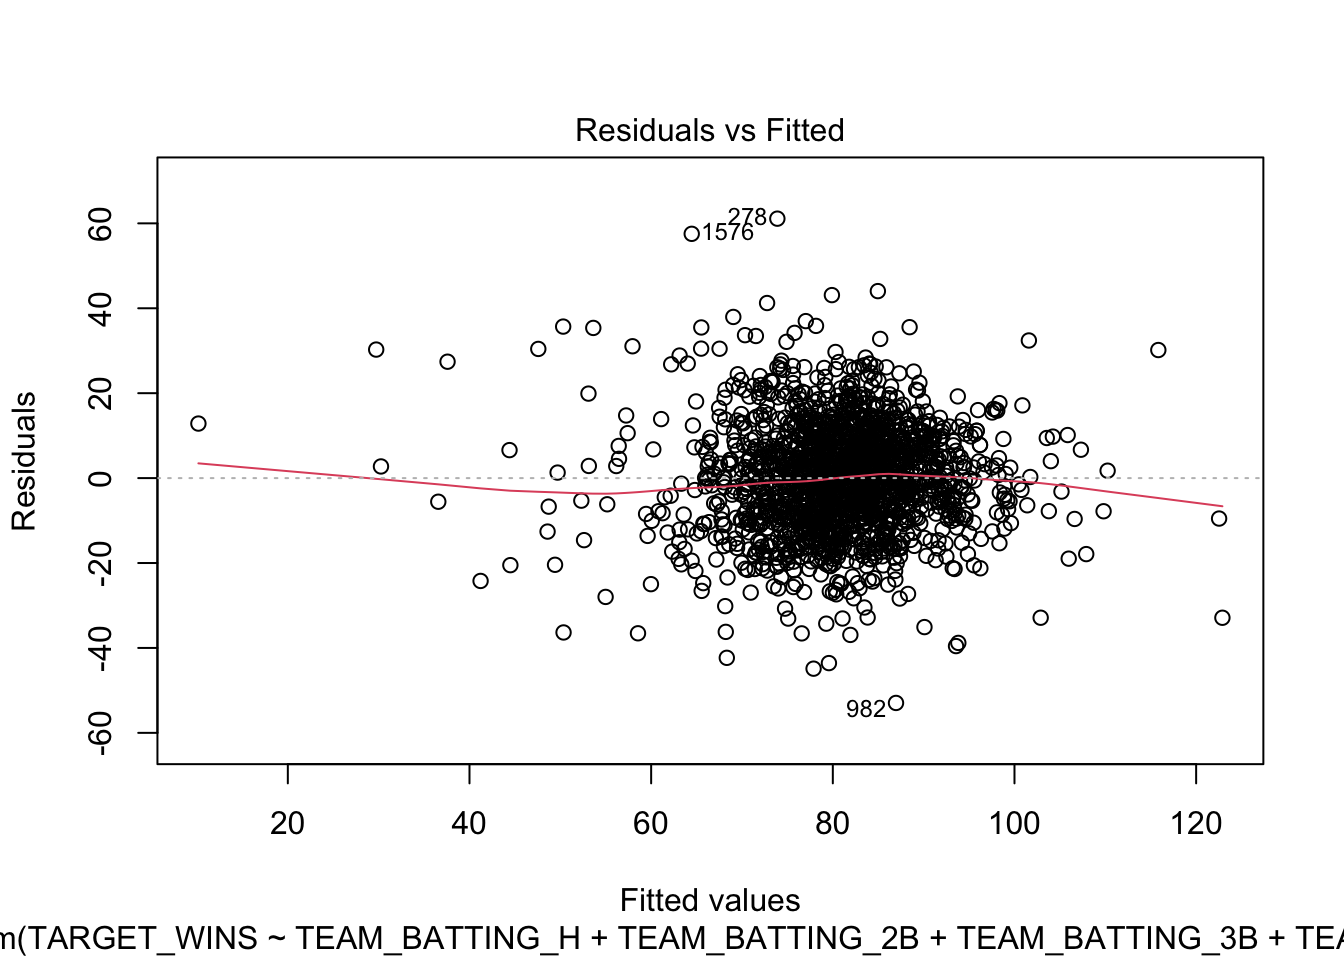
\includegraphics{Assignment1_Data621_HW_files/figure-latex/model-4-diagnostic-ph plots-1.pdf}
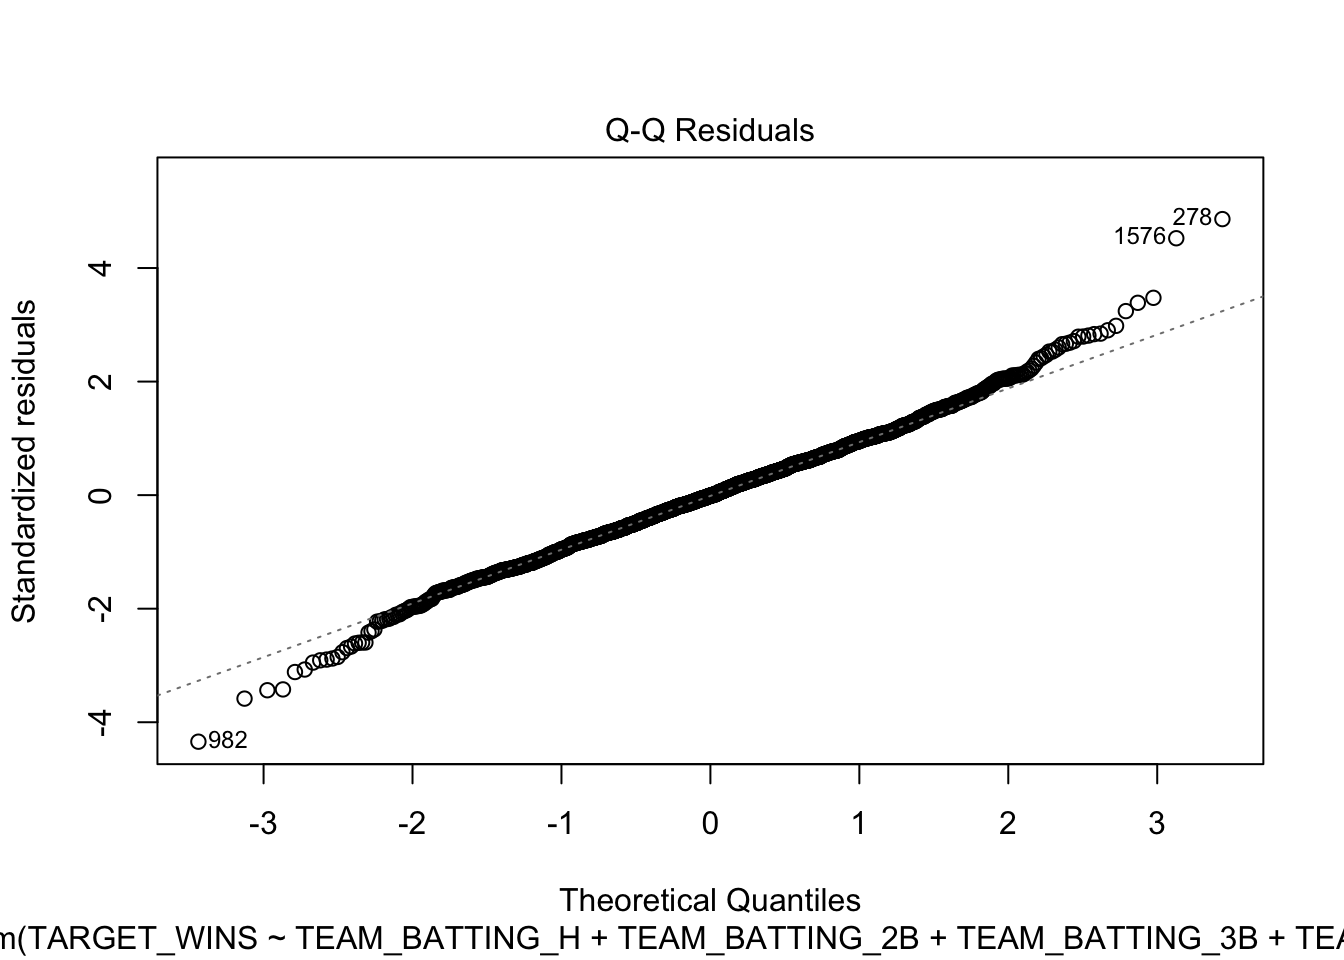
\includegraphics{Assignment1_Data621_HW_files/figure-latex/model-4-diagnostic-ph plots-2.pdf}
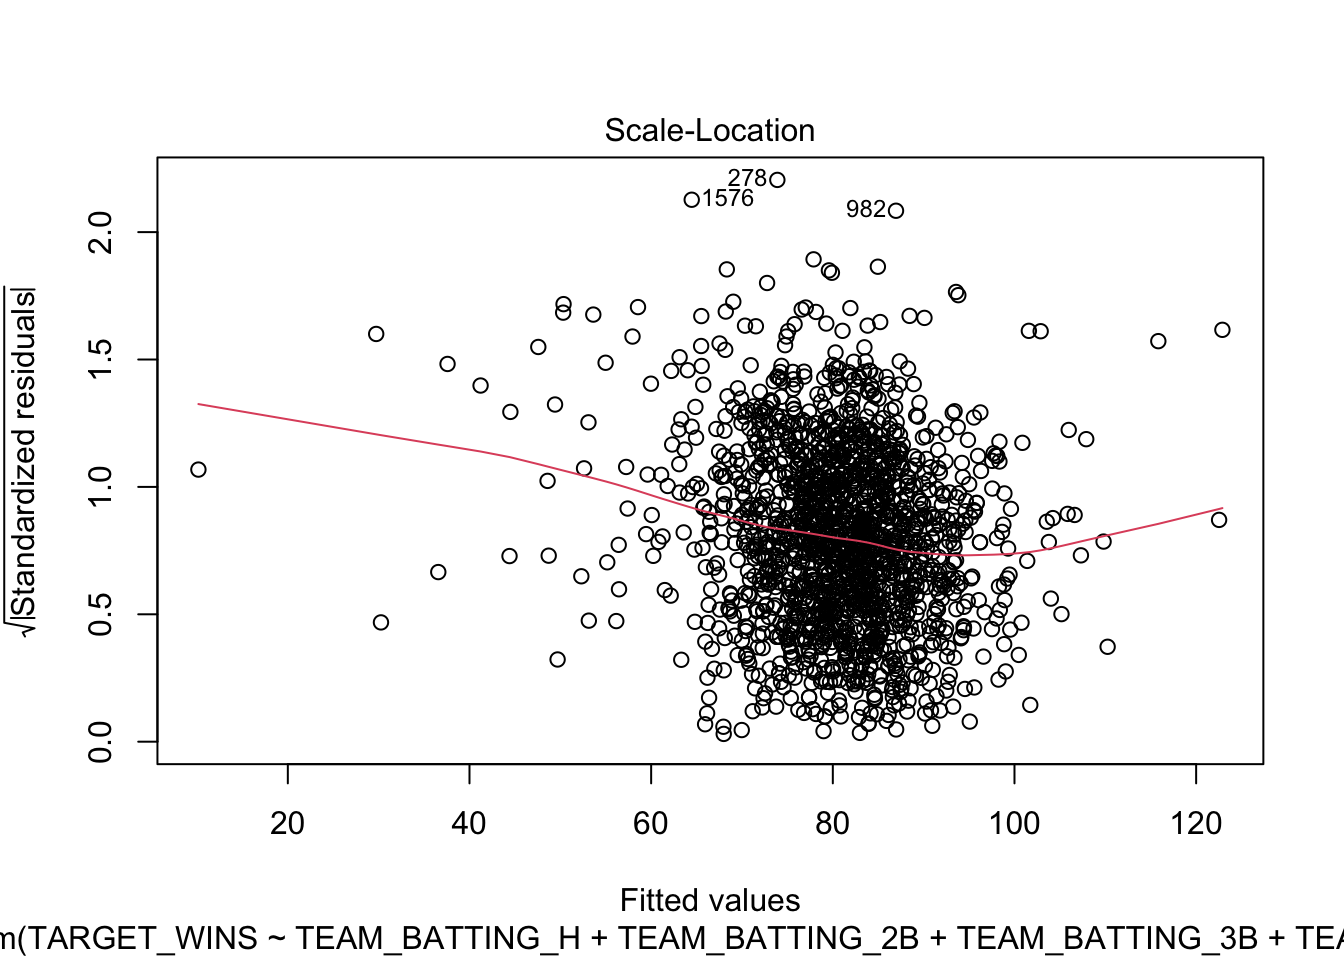
\includegraphics{Assignment1_Data621_HW_files/figure-latex/model-4-diagnostic-ph plots-3.pdf}
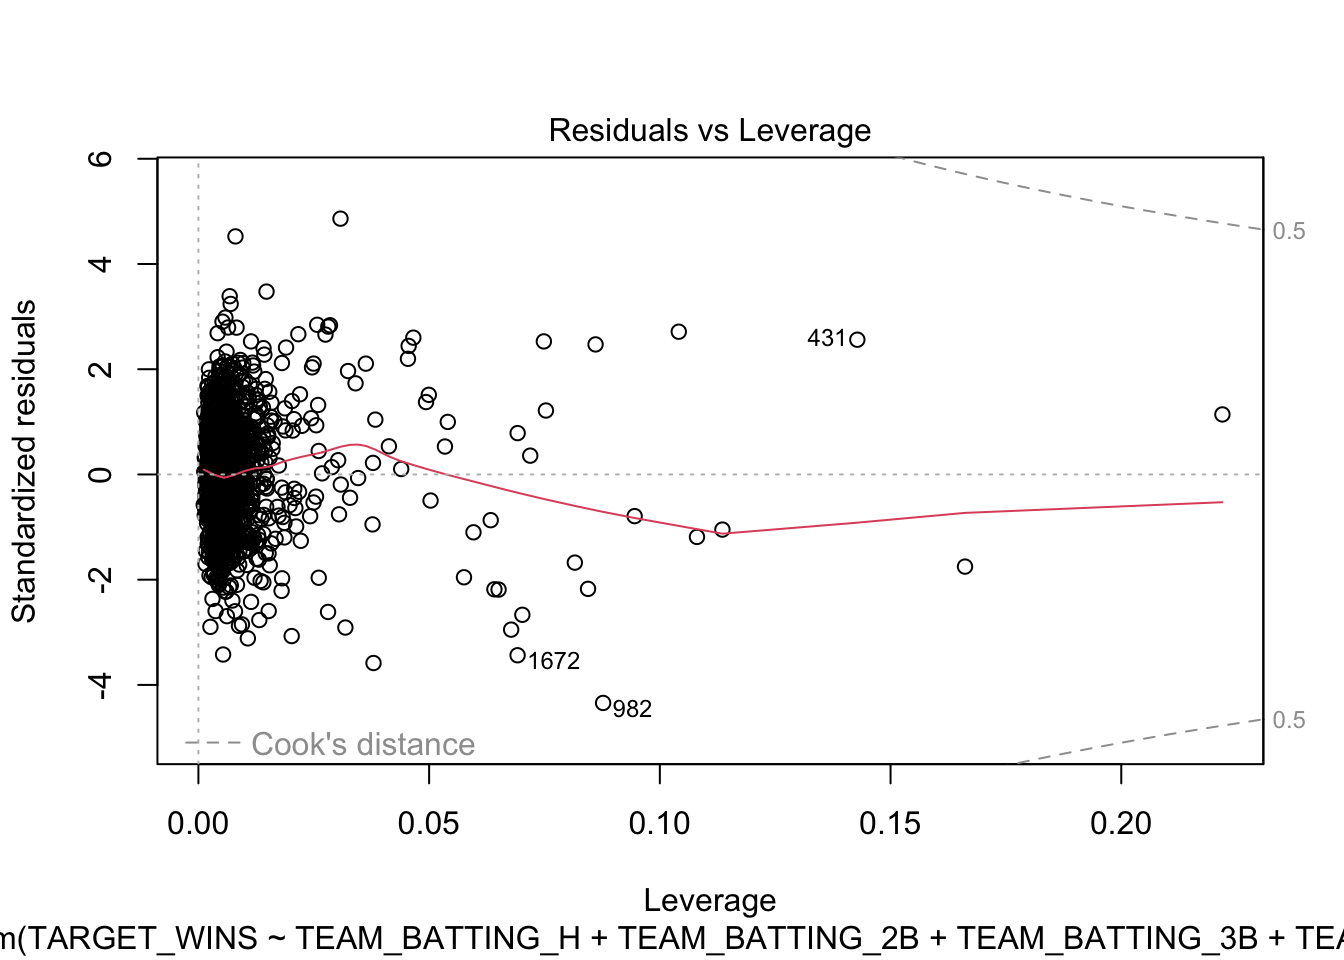
\includegraphics{Assignment1_Data621_HW_files/figure-latex/model-4-diagnostic-ph plots-4.pdf}

\subparagraph{Multicolinearity}\label{multicolinearity-1}

A VIF Test shows several variables that are highly correlated, including
TEAM\_PITCHING\_H, TEAM\_BATTING\_BB, TEAM\_PITCHING\_SO,
TEAM\_PITCHING\_BB, TEAM\_FIELDING\_E \& TEAM\_BATTING\_H. We may choose
to leave these out.

\begin{Shaded}
\begin{Highlighting}[]
\FunctionTok{vif}\NormalTok{(stp\_logx\_model)}
\end{Highlighting}
\end{Shaded}

\begin{verbatim}
##      TEAM_BATTING_2B      TEAM_BATTING_3B      TEAM_BATTING_BB 
##             2.628155             2.803296             7.877815 
##      TEAM_BATTING_SO      TEAM_BASERUN_SB     TEAM_PITCHING_HR 
##            14.385392             1.735966             9.361936 
##      TEAM_FIELDING_E     TEAM_FIELDING_DP   log_TEAM_BATTING_H 
##             4.073234             1.464900             4.298651 
##  log_TEAM_BATTING_HR log_TEAM_PITCHING_SO log_TEAM_PITCHING_BB 
##            10.786426            10.955741             5.533907
\end{verbatim}

\subparagraph{Diagnosing our Model}\label{diagnosing-our-model-3}

Linearity

\begin{Shaded}
\begin{Highlighting}[]
\FunctionTok{plot}\NormalTok{(stp\_logx\_model, }\AttributeTok{which=}\DecValTok{1}\NormalTok{)}
\end{Highlighting}
\end{Shaded}

\includegraphics{Assignment1_Data621_HW_files/figure-latex/unnamed-chunk-55-1.pdf}

Our Residuals vs.~Fitted plot suggest a fairly linear model.

Normality

\begin{Shaded}
\begin{Highlighting}[]
\FunctionTok{plot}\NormalTok{(stp\_logx\_model, }\AttributeTok{which =} \DecValTok{2}\NormalTok{)}
\end{Highlighting}
\end{Shaded}

\includegraphics{Assignment1_Data621_HW_files/figure-latex/unnamed-chunk-56-1.pdf}

\begin{Shaded}
\begin{Highlighting}[]
\CommentTok{\# Shapiro{-}Wilk normality test: look for high p{-}value}
\FunctionTok{shapiro.test}\NormalTok{(}\FunctionTok{residuals}\NormalTok{(stp\_logx\_model))}
\end{Highlighting}
\end{Shaded}

\begin{verbatim}
## 
##  Shapiro-Wilk normality test
## 
## data:  residuals(stp_logx_model)
## W = 0.9961, p-value = 0.000232
\end{verbatim}

Our QQ plot suggests normality thought there is some skewing on the
tails, particularly on the right. The skewing appears to be less pitched
than in our backward-selected model or Box-Cox Transformed model.

A Shapiro Wilk's Test statistic had a value of 0.9943, also suggesting
normality. However, since the p-value (4.273e-06) is less than
\textless{} 0.05 we may still be violating our normality assumption.

Heteroscedasticity

\includegraphics{Assignment1_Data621_HW_files/figure-latex/unnamed-chunk-57-1.pdf}
\includegraphics{Assignment1_Data621_HW_files/figure-latex/unnamed-chunk-57-2.pdf}

\begin{verbatim}
## 
##  studentized Breusch-Pagan test
## 
## data:  stp_logx_model
## BP = 233.06, df = 12, p-value < 2.2e-16
\end{verbatim}

Our Scale-Location plot shows that points appear somewhat evenly
distributed above and below the trend line but there is clear bowing in
the trend line, suggesting that the variance of the residuals is not
constant and therefore heteroschedastic. While there is no obvious
fan/wedge pattern, there is clustering in the center suggesting
underfitting, high leverage outliers or that additional transformation
may be needed. As our Cook's Distance plot has no values with a greater
than 1, we can rule our the effects of high leverage points.

The Breusch-Page test statistic BP (302.21) and the small p-value
(2.2e-16) suggest evidence of heteroscedasticity. Though the values are
different that we may need to transform the data to meet the Assumption
of Homoscedasticity.

Independence

\begin{Shaded}
\begin{Highlighting}[]
\FunctionTok{acf}\NormalTok{(}\FunctionTok{residuals}\NormalTok{(stp\_logx\_model))}
\end{Highlighting}
\end{Shaded}

\includegraphics{Assignment1_Data621_HW_files/figure-latex/unnamed-chunk-58-1.pdf}

\begin{Shaded}
\begin{Highlighting}[]
\FunctionTok{durbinWatsonTest}\NormalTok{(stp\_logx\_model)}
\end{Highlighting}
\end{Shaded}

\begin{verbatim}
##  lag Autocorrelation D-W Statistic p-value
##    1     -0.01529779      2.029836   0.574
##  Alternative hypothesis: rho != 0
\end{verbatim}

\begin{Shaded}
\begin{Highlighting}[]
\CommentTok{\# Durbin Watson should be close to 2}
\end{Highlighting}
\end{Shaded}

Our Autocorrelation Function shows that there are lags above the blue
dashed line, suggesting no autocorrelation. This is confirmed through a
Durbin-Watson test statistic value of 2.011 and an autocorrelation value
of -0.008. Furthermore, as our p-value (0.822) is greater than 0.05, we
do not have enough evidence to reject the null hypothesis that there is
no autocorrelation. In other words, the test results suggest that our
model's residuals are independent and therefore do not violate the
Independence Assumption.

\paragraph{Model T5: Box-Cox Transformation on Dependent
Variable}\label{model-t5-box-cox-transformation-on-dependent-variable}

In this section, we apply a Box-Cox Transformation to our backward
selected mode and data.

\begin{Shaded}
\begin{Highlighting}[]
\NormalTok{stpbc\_model }\OtherTok{\textless{}{-}} \FunctionTok{boxcox}\NormalTok{(back\_select\_model, }\AttributeTok{lambda =} \FunctionTok{seq}\NormalTok{(}\SpecialCharTok{{-}}\DecValTok{3}\NormalTok{,}\DecValTok{3}\NormalTok{))}
\end{Highlighting}
\end{Shaded}

\includegraphics{Assignment1_Data621_HW_files/figure-latex/model4-boxcox-1.pdf}

\begin{Shaded}
\begin{Highlighting}[]
\FunctionTok{plot}\NormalTok{(stpbc\_model)}
\end{Highlighting}
\end{Shaded}

\includegraphics{Assignment1_Data621_HW_files/figure-latex/model4-boxcox-2.pdf}

\begin{Shaded}
\begin{Highlighting}[]
\NormalTok{best\_lambda }\OtherTok{\textless{}{-}}\NormalTok{ stpbc\_model}\SpecialCharTok{$}\NormalTok{x[}\FunctionTok{which}\NormalTok{(stpbc\_model}\SpecialCharTok{$}\NormalTok{y}\SpecialCharTok{==}\FunctionTok{max}\NormalTok{(stpbc\_model}\SpecialCharTok{$}\NormalTok{y))]}
 
\NormalTok{stp\_model\_inv }\OtherTok{\textless{}{-}} \FunctionTok{lm}\NormalTok{((TARGET\_WINS)}\SpecialCharTok{\^{}}\NormalTok{best\_lambda }\SpecialCharTok{\textasciitilde{}}\NormalTok{ TEAM\_BATTING\_H }\SpecialCharTok{+}\NormalTok{ TEAM\_BATTING\_2B }\SpecialCharTok{+}\NormalTok{ TEAM\_BATTING\_3B }\SpecialCharTok{+}\NormalTok{ TEAM\_BATTING\_SO }\SpecialCharTok{+}\NormalTok{ TEAM\_BASERUN\_SB }\SpecialCharTok{+}\NormalTok{ TEAM\_PITCHING\_HR }\SpecialCharTok{+}\NormalTok{ TEAM\_PITCHING\_BB }\SpecialCharTok{+}\NormalTok{ TEAM\_PITCHING\_SO }\SpecialCharTok{+}\NormalTok{ TEAM\_FIELDING\_E }\SpecialCharTok{+}\NormalTok{ TEAM\_FIELDING\_DP, }\AttributeTok{data =}\NormalTok{ stp75\_train\_df)}

\FunctionTok{summary}\NormalTok{(stp\_model\_inv)}
\end{Highlighting}
\end{Shaded}

\begin{verbatim}
## 
## Call:
## lm(formula = (TARGET_WINS)^best_lambda ~ TEAM_BATTING_H + TEAM_BATTING_2B + 
##     TEAM_BATTING_3B + TEAM_BATTING_SO + TEAM_BASERUN_SB + TEAM_PITCHING_HR + 
##     TEAM_PITCHING_BB + TEAM_PITCHING_SO + TEAM_FIELDING_E + TEAM_FIELDING_DP, 
##     data = stp75_train_df)
## 
## Residuals:
##      Min       1Q   Median       3Q      Max 
## -160.002  -31.694   -1.753   30.262  218.369 
## 
## Coefficients:
##                   Estimate Std. Error t value Pr(>|t|)    
## (Intercept)      30.439025  22.090363   1.378    0.168    
## TEAM_BATTING_H    0.168744   0.015834  10.657  < 2e-16 ***
## TEAM_BATTING_2B  -0.049023   0.038413  -1.276    0.202    
## TEAM_BATTING_3B   0.280560   0.068908   4.072 4.89e-05 ***
## TEAM_BATTING_SO  -0.005103   0.013188  -0.387    0.699    
## TEAM_BASERUN_SB   0.107337   0.017380   6.176 8.22e-10 ***
## TEAM_PITCHING_HR  0.182375   0.036190   5.039 5.17e-07 ***
## TEAM_PITCHING_BB  0.003137   0.009882   0.317    0.751    
## TEAM_PITCHING_SO -0.002248   0.007738  -0.291    0.771    
## TEAM_FIELDING_E  -0.086413   0.008583 -10.068  < 2e-16 ***
## TEAM_FIELDING_DP -0.371205   0.052845  -7.024 3.10e-12 ***
## ---
## Signif. codes:  0 '***' 0.001 '**' 0.01 '*' 0.05 '.' 0.1 ' ' 1
## 
## Residual standard error: 47.18 on 1691 degrees of freedom
## Multiple R-squared:  0.2928, Adjusted R-squared:  0.2886 
## F-statistic: 70.02 on 10 and 1691 DF,  p-value: < 2.2e-16
\end{verbatim}

Looking at the summary of our new Box-Cox transformed model shows three
variables are not statistically significant. We should therefore remove
them one at a time.

\begin{Shaded}
\begin{Highlighting}[]
\NormalTok{stp\_model\_inv }\OtherTok{\textless{}{-}} \FunctionTok{update}\NormalTok{(stp\_model\_inv, . }\SpecialCharTok{\textasciitilde{}}\NormalTok{ . }\SpecialCharTok{{-}}\NormalTok{ TEAM\_BATTING\_SO)}
\FunctionTok{summary}\NormalTok{(stp\_model\_inv)}
\end{Highlighting}
\end{Shaded}

\begin{verbatim}
## 
## Call:
## lm(formula = (TARGET_WINS)^best_lambda ~ TEAM_BATTING_H + TEAM_BATTING_2B + 
##     TEAM_BATTING_3B + TEAM_BASERUN_SB + TEAM_PITCHING_HR + TEAM_PITCHING_BB + 
##     TEAM_PITCHING_SO + TEAM_FIELDING_E + TEAM_FIELDING_DP, data = stp75_train_df)
## 
## Residuals:
##      Min       1Q   Median       3Q      Max 
## -159.912  -31.656   -1.876   30.221  217.584 
## 
## Coefficients:
##                   Estimate Std. Error t value Pr(>|t|)    
## (Intercept)      25.274155  17.597392   1.436    0.151    
## TEAM_BATTING_H    0.170846   0.014870  11.490  < 2e-16 ***
## TEAM_BATTING_2B  -0.051759   0.037748  -1.371    0.170    
## TEAM_BATTING_3B   0.285658   0.067620   4.224 2.52e-05 ***
## TEAM_BASERUN_SB   0.104773   0.016063   6.523 9.10e-11 ***
## TEAM_PITCHING_HR  0.175985   0.032194   5.466 5.28e-08 ***
## TEAM_PITCHING_BB  0.004891   0.008778   0.557    0.577    
## TEAM_PITCHING_SO -0.004313   0.005602  -0.770    0.441    
## TEAM_FIELDING_E  -0.084844   0.007563 -11.218  < 2e-16 ***
## TEAM_FIELDING_DP -0.371106   0.052831  -7.024 3.10e-12 ***
## ---
## Signif. codes:  0 '***' 0.001 '**' 0.01 '*' 0.05 '.' 0.1 ' ' 1
## 
## Residual standard error: 47.17 on 1692 degrees of freedom
## Multiple R-squared:  0.2928, Adjusted R-squared:  0.289 
## F-statistic: 77.82 on 9 and 1692 DF,  p-value: < 2.2e-16
\end{verbatim}

\begin{Shaded}
\begin{Highlighting}[]
\FunctionTok{AIC}\NormalTok{(back\_select\_model)}
\end{Highlighting}
\end{Shaded}

\begin{verbatim}
## [1] 13605.45
\end{verbatim}

\begin{Shaded}
\begin{Highlighting}[]
\NormalTok{stp\_model\_inv }\OtherTok{\textless{}{-}} \FunctionTok{update}\NormalTok{(stp\_model\_inv, . }\SpecialCharTok{\textasciitilde{}}\NormalTok{ . }\SpecialCharTok{{-}}\NormalTok{ TEAM\_PITCHING\_BB)}
\FunctionTok{summary}\NormalTok{(stp\_model\_inv)}
\end{Highlighting}
\end{Shaded}

\begin{verbatim}
## 
## Call:
## lm(formula = (TARGET_WINS)^best_lambda ~ TEAM_BATTING_H + TEAM_BATTING_2B + 
##     TEAM_BATTING_3B + TEAM_BASERUN_SB + TEAM_PITCHING_HR + TEAM_PITCHING_SO + 
##     TEAM_FIELDING_E + TEAM_FIELDING_DP, data = stp75_train_df)
## 
## Residuals:
##      Min       1Q   Median       3Q      Max 
## -159.945  -31.724   -1.658   30.724  216.857 
## 
## Coefficients:
##                   Estimate Std. Error t value Pr(>|t|)    
## (Intercept)      25.545291  17.587082   1.453    0.147    
## TEAM_BATTING_H    0.171217   0.014852  11.528  < 2e-16 ***
## TEAM_BATTING_2B  -0.052598   0.037710  -1.395    0.163    
## TEAM_BATTING_3B   0.290885   0.066952   4.345 1.48e-05 ***
## TEAM_BASERUN_SB   0.106926   0.015588   6.860 9.65e-12 ***
## TEAM_PITCHING_HR  0.180261   0.031260   5.767 9.60e-09 ***
## TEAM_PITCHING_SO -0.003855   0.005540  -0.696    0.487    
## TEAM_FIELDING_E  -0.085052   0.007553 -11.261  < 2e-16 ***
## TEAM_FIELDING_DP -0.365976   0.052012  -7.036 2.85e-12 ***
## ---
## Signif. codes:  0 '***' 0.001 '**' 0.01 '*' 0.05 '.' 0.1 ' ' 1
## 
## Residual standard error: 47.16 on 1693 degrees of freedom
## Multiple R-squared:  0.2926, Adjusted R-squared:  0.2893 
## F-statistic: 87.54 on 8 and 1693 DF,  p-value: < 2.2e-16
\end{verbatim}

\begin{Shaded}
\begin{Highlighting}[]
\FunctionTok{AIC}\NormalTok{(back\_select\_model)}
\end{Highlighting}
\end{Shaded}

\begin{verbatim}
## [1] 13605.45
\end{verbatim}

\begin{Shaded}
\begin{Highlighting}[]
\NormalTok{stp\_model\_inv }\OtherTok{\textless{}{-}} \FunctionTok{update}\NormalTok{(stp\_model\_inv, . }\SpecialCharTok{\textasciitilde{}}\NormalTok{ . }\SpecialCharTok{{-}}\NormalTok{ TEAM\_PITCHING\_SO)}
\FunctionTok{summary}\NormalTok{(stp\_model\_inv)}
\end{Highlighting}
\end{Shaded}

\begin{verbatim}
## 
## Call:
## lm(formula = (TARGET_WINS)^best_lambda ~ TEAM_BATTING_H + TEAM_BATTING_2B + 
##     TEAM_BATTING_3B + TEAM_BASERUN_SB + TEAM_PITCHING_HR + TEAM_FIELDING_E + 
##     TEAM_FIELDING_DP, data = stp75_train_df)
## 
## Residuals:
##      Min       1Q   Median       3Q      Max 
## -159.684  -31.752   -1.647   30.624  215.869 
## 
## Coefficients:
##                   Estimate Std. Error t value Pr(>|t|)    
## (Intercept)      17.875917  13.703459   1.304    0.192    
## TEAM_BATTING_H    0.176195   0.013013  13.540  < 2e-16 ***
## TEAM_BATTING_2B  -0.059243   0.036475  -1.624    0.105    
## TEAM_BATTING_3B   0.295325   0.066638   4.432 9.94e-06 ***
## TEAM_BASERUN_SB   0.105857   0.015510   6.825 1.22e-11 ***
## TEAM_PITCHING_HR  0.169940   0.027513   6.177 8.18e-10 ***
## TEAM_FIELDING_E  -0.087586   0.006616 -13.239  < 2e-16 ***
## TEAM_FIELDING_DP -0.363023   0.051830  -7.004 3.57e-12 ***
## ---
## Signif. codes:  0 '***' 0.001 '**' 0.01 '*' 0.05 '.' 0.1 ' ' 1
## 
## Residual standard error: 47.15 on 1694 degrees of freedom
## Multiple R-squared:  0.2924, Adjusted R-squared:  0.2895 
## F-statistic:   100 on 7 and 1694 DF,  p-value: < 2.2e-16
\end{verbatim}

\begin{Shaded}
\begin{Highlighting}[]
\FunctionTok{AIC}\NormalTok{(back\_select\_model)}
\end{Highlighting}
\end{Shaded}

\begin{verbatim}
## [1] 13605.45
\end{verbatim}

\begin{Shaded}
\begin{Highlighting}[]
\NormalTok{stp\_model\_inv }\OtherTok{\textless{}{-}} \FunctionTok{update}\NormalTok{(stp\_model\_inv, . }\SpecialCharTok{\textasciitilde{}}\NormalTok{ . }\SpecialCharTok{{-}}\NormalTok{ TEAM\_BATTING\_2B)}
\FunctionTok{summary}\NormalTok{(stp\_model\_inv)}
\end{Highlighting}
\end{Shaded}

\begin{verbatim}
## 
## Call:
## lm(formula = (TARGET_WINS)^best_lambda ~ TEAM_BATTING_H + TEAM_BATTING_3B + 
##     TEAM_BASERUN_SB + TEAM_PITCHING_HR + TEAM_FIELDING_E + TEAM_FIELDING_DP, 
##     data = stp75_train_df)
## 
## Residuals:
##      Min       1Q   Median       3Q      Max 
## -156.515  -32.052   -1.391   30.475  210.291 
## 
## Coefficients:
##                   Estimate Std. Error t value Pr(>|t|)    
## (Intercept)      22.357240  13.429300   1.665   0.0961 .  
## TEAM_BATTING_H    0.162907   0.010124  16.091  < 2e-16 ***
## TEAM_BATTING_3B   0.308245   0.066193   4.657 3.46e-06 ***
## TEAM_BASERUN_SB   0.107080   0.015499   6.909 6.89e-12 ***
## TEAM_PITCHING_HR  0.161572   0.027039   5.975 2.79e-09 ***
## TEAM_FIELDING_E  -0.084195   0.006281 -13.405  < 2e-16 ***
## TEAM_FIELDING_DP -0.363575   0.051854  -7.011 3.39e-12 ***
## ---
## Signif. codes:  0 '***' 0.001 '**' 0.01 '*' 0.05 '.' 0.1 ' ' 1
## 
## Residual standard error: 47.18 on 1695 degrees of freedom
## Multiple R-squared:  0.2913, Adjusted R-squared:  0.2888 
## F-statistic: 116.1 on 6 and 1695 DF,  p-value: < 2.2e-16
\end{verbatim}

\begin{Shaded}
\begin{Highlighting}[]
\FunctionTok{AIC}\NormalTok{(back\_select\_model)}
\end{Highlighting}
\end{Shaded}

\begin{verbatim}
## [1] 13605.45
\end{verbatim}

\subparagraph{Diagnosing our Model}\label{diagnosing-our-model-4}

Linearity

\begin{Shaded}
\begin{Highlighting}[]
\FunctionTok{plot}\NormalTok{(stp\_model\_inv, }\AttributeTok{which=}\DecValTok{1}\NormalTok{)}
\end{Highlighting}
\end{Shaded}

\includegraphics{Assignment1_Data621_HW_files/figure-latex/unnamed-chunk-60-1.pdf}

Our Residuals vs.~Fitted plot suggest a fairly linear model.

Normality

\begin{Shaded}
\begin{Highlighting}[]
\FunctionTok{plot}\NormalTok{(stp\_model\_inv, }\AttributeTok{which =} \DecValTok{2}\NormalTok{)}
\end{Highlighting}
\end{Shaded}

\includegraphics{Assignment1_Data621_HW_files/figure-latex/unnamed-chunk-61-1.pdf}

\begin{Shaded}
\begin{Highlighting}[]
\FunctionTok{shapiro.test}\NormalTok{(}\FunctionTok{residuals}\NormalTok{(stp\_model\_inv))}
\end{Highlighting}
\end{Shaded}

\begin{verbatim}
## 
##  Shapiro-Wilk normality test
## 
## data:  residuals(stp_model_inv)
## W = 0.99631, p-value = 0.0003925
\end{verbatim}

\begin{Shaded}
\begin{Highlighting}[]
\CommentTok{\# Shapiro{-}Wilk normality test: look for high p{-}value}
\end{Highlighting}
\end{Shaded}

Our QQ plot suggests normality thought there is obvious skewing on the
tails, particularly on the right.

A Shapiro Wilk's Test statistic had a value of 0.996, also suggesting
normality. However, since the p-value (7.132e-05) is less than
\textless{} 0.05 we may still be violating our normality assumption.

Heteroscedasticity

\includegraphics{Assignment1_Data621_HW_files/figure-latex/unnamed-chunk-62-1.pdf}
\includegraphics{Assignment1_Data621_HW_files/figure-latex/unnamed-chunk-62-2.pdf}

\begin{verbatim}
## 
##  studentized Breusch-Pagan test
## 
## data:  stp_model_inv
## BP = 154.07, df = 6, p-value < 2.2e-16
\end{verbatim}

Our Scale-Location plot shows that points appear somewhat evenly
distributed above and below the trend line. While there is no obvious
fan/wedge pattern, there is clustering in the center suggesting
underfitting, high leverage outliers or that additional transformation
may be needed. As our Cook's Distance plot has no values with a greater
than 1, we can rule our the effects of high leverage points.

The Breusch-Page test statistic BP (176.76) and the small p-value
(2.2e-16) suggest evidence of heteroscedasticity. Though the values are
different that we may need to transform the data to meet the Assumption
of Homoscedasticity.

Independence

\begin{Shaded}
\begin{Highlighting}[]
\FunctionTok{acf}\NormalTok{(}\FunctionTok{residuals}\NormalTok{(stp\_model\_inv))}
\end{Highlighting}
\end{Shaded}

\includegraphics{Assignment1_Data621_HW_files/figure-latex/unnamed-chunk-63-1.pdf}

\begin{Shaded}
\begin{Highlighting}[]
\FunctionTok{durbinWatsonTest}\NormalTok{(stp\_model\_inv)}
\end{Highlighting}
\end{Shaded}

\begin{verbatim}
##  lag Autocorrelation D-W Statistic p-value
##    1     -0.01014699      2.019358   0.674
##  Alternative hypothesis: rho != 0
\end{verbatim}

\begin{Shaded}
\begin{Highlighting}[]
\CommentTok{\# Durbin Watson should be close to 2}
\end{Highlighting}
\end{Shaded}

Our Autocorrelation Function shows that there are lags above the blue
dashed line, suggesting no autocorrelation. This is confirmed through a
Durbin-Watson test statistic value of 2.03 and an autocorrelation value
of -0.021. Furthermore, as our p-value (0.416) is greater than 0.05, we
do not have enough evidence to reject the null hypothesis that there is
no autocorrelation. In other words, the test results suggest that our
model's residuals are independent and therefore do not violate the
Independence Assumption.

\emph{Conclusion} Applying a Box-Cox transformation to our model appears
does not seem to have improved the results of our backward selected
model. This model continues to violate the Homoscedasticity Assumption
and has mixed results for our Normality Assumption.

\subsubsection{Advanced Techniques}\label{advanced-techniques}

\paragraph{Model A1: Lasso Regression}\label{model-a1-lasso-regression}

The Least Absolute Shrinkage and Selection Operator (LASSO) selection
method uses a shrinkage approach to determining the optimal predictors
by attempting to find a balance between simplicity and accuracy.It
applies a penalty to the standard linear regression model to encourage
the coefficients of features with weak influence to equal zero to
prevent overfitting.

\begin{Shaded}
\begin{Highlighting}[]
\NormalTok{x }\OtherTok{=} \FunctionTok{model.matrix}\NormalTok{(TARGET\_WINS }\SpecialCharTok{\textasciitilde{}}\NormalTok{ ., }\AttributeTok{data =}\NormalTok{ stp75\_train\_df)}
\NormalTok{y }\OtherTok{=}\NormalTok{ stp75\_train\_df}\SpecialCharTok{$}\NormalTok{TARGET\_WINS}

\NormalTok{fit\_lasso }\OtherTok{=} \FunctionTok{glmnet}\NormalTok{(x, y, }\AttributeTok{alpha=}\DecValTok{1}\NormalTok{)}
\FunctionTok{plot}\NormalTok{(fit\_lasso, }\AttributeTok{xvar=}\StringTok{"lambda"}\NormalTok{, }\AttributeTok{label=}\ConstantTok{TRUE}\NormalTok{)}
\end{Highlighting}
\end{Shaded}

\includegraphics{Assignment1_Data621_HW_files/figure-latex/unnamed-chunk-64-1.pdf}

\begin{Shaded}
\begin{Highlighting}[]
\NormalTok{cv\_lasso }\OtherTok{=} \FunctionTok{cv.glmnet}\NormalTok{(x,y,}\AttributeTok{alpha=}\DecValTok{1}\NormalTok{)}
\CommentTok{\#plot(cv.lasso)}
\FunctionTok{coef}\NormalTok{(cv\_lasso)}
\end{Highlighting}
\end{Shaded}

\begin{verbatim}
## 16 x 1 sparse Matrix of class "dgCMatrix"
##                             s1
## (Intercept)      19.5221297165
## (Intercept)       .           
## TEAM_BATTING_H    0.0431544433
## TEAM_BATTING_2B   .           
## TEAM_BATTING_3B   0.0173524152
## TEAM_BATTING_HR   0.0121590365
## TEAM_BATTING_BB   0.0105502074
## TEAM_BATTING_SO   .           
## TEAM_BASERUN_SB   0.0172781093
## TEAM_BASERUN_CS   .           
## TEAM_PITCHING_H  -0.0002011034
## TEAM_PITCHING_HR  .           
## TEAM_PITCHING_BB  .           
## TEAM_PITCHING_SO  .           
## TEAM_FIELDING_E  -0.0128248793
## TEAM_FIELDING_DP -0.0569377921
\end{verbatim}

Performing LASSO on our training subset -- 75\% of full training set
with log transformation applied -- gives us 7 predictors: -
TEAM\_BATTING\_H - TEAM\_BATTING\_3B - TEAM\_BATTING\_BB -
TEAM\_BASERUN\_SB - TEAM\_PITCHING\_HR - TEAM\_FIELDING\_E -
TEAM\_FIELDING\_DP

\begin{Shaded}
\begin{Highlighting}[]
\NormalTok{lasso\_model }\OtherTok{\textless{}{-}} \FunctionTok{lm}\NormalTok{(TARGET\_WINS }\SpecialCharTok{\textasciitilde{}}\NormalTok{ TEAM\_BATTING\_H }\SpecialCharTok{+}\NormalTok{ TEAM\_BATTING\_3B }\SpecialCharTok{+}\NormalTok{ TEAM\_BATTING\_BB }\SpecialCharTok{+}\NormalTok{ TEAM\_BASERUN\_SB }\SpecialCharTok{+}\NormalTok{ TEAM\_PITCHING\_HR }\SpecialCharTok{+}\NormalTok{ TEAM\_FIELDING\_E }\SpecialCharTok{+}\NormalTok{ TEAM\_FIELDING\_DP, }\AttributeTok{data =}\NormalTok{ stp75\_train\_df)}

\FunctionTok{summary}\NormalTok{(lasso\_model)}
\end{Highlighting}
\end{Shaded}

\begin{verbatim}
## 
## Call:
## lm(formula = TARGET_WINS ~ TEAM_BATTING_H + TEAM_BATTING_3B + 
##     TEAM_BATTING_BB + TEAM_BASERUN_SB + TEAM_PITCHING_HR + TEAM_FIELDING_E + 
##     TEAM_FIELDING_DP, data = stp75_train_df)
## 
## Residuals:
##     Min      1Q  Median      3Q     Max 
## -47.063  -8.718  -0.031   8.628  56.109 
## 
## Coefficients:
##                   Estimate Std. Error t value Pr(>|t|)    
## (Intercept)      17.688724   3.979040   4.445 9.34e-06 ***
## TEAM_BATTING_H    0.045567   0.002825  16.129  < 2e-16 ***
## TEAM_BATTING_3B   0.083852   0.018519   4.528 6.38e-06 ***
## TEAM_BATTING_BB   0.010914   0.003865   2.824   0.0048 ** 
## TEAM_BASERUN_SB   0.026415   0.004559   5.794 8.20e-09 ***
## TEAM_PITCHING_HR  0.040350   0.007740   5.213 2.09e-07 ***
## TEAM_FIELDING_E  -0.021314   0.002205  -9.666  < 2e-16 ***
## TEAM_FIELDING_DP -0.111953   0.014899  -7.514 9.21e-14 ***
## ---
## Signif. codes:  0 '***' 0.001 '**' 0.01 '*' 0.05 '.' 0.1 ' ' 1
## 
## Residual standard error: 13.16 on 1694 degrees of freedom
## Multiple R-squared:  0.2998, Adjusted R-squared:  0.2969 
## F-statistic: 103.6 on 7 and 1694 DF,  p-value: < 2.2e-16
\end{verbatim}

\begin{Shaded}
\begin{Highlighting}[]
\FunctionTok{vif}\NormalTok{(lasso\_model)}
\end{Highlighting}
\end{Shaded}

\begin{verbatim}
##   TEAM_BATTING_H  TEAM_BATTING_3B  TEAM_BATTING_BB  TEAM_BASERUN_SB 
##         1.637967         2.557648         2.158278         1.524902 
## TEAM_PITCHING_HR  TEAM_FIELDING_E TEAM_FIELDING_DP 
##         2.251225         2.351028         1.326869
\end{verbatim}

Our VIF test shows no strong correlation between predictors.

\subparagraph{Testing Our Assumptions}\label{testing-our-assumptions}

Linearity

\begin{Shaded}
\begin{Highlighting}[]
\FunctionTok{plot}\NormalTok{(lasso\_model, }\AttributeTok{which=}\DecValTok{1}\NormalTok{)}
\end{Highlighting}
\end{Shaded}

\includegraphics{Assignment1_Data621_HW_files/figure-latex/unnamed-chunk-65-1.pdf}

Our Residuals vs.~Fitted plot suggest a fairly linear model.

Normality

\begin{Shaded}
\begin{Highlighting}[]
\FunctionTok{plot}\NormalTok{(lasso\_model, }\AttributeTok{which =} \DecValTok{2}\NormalTok{)}
\end{Highlighting}
\end{Shaded}

\includegraphics{Assignment1_Data621_HW_files/figure-latex/unnamed-chunk-66-1.pdf}

\begin{Shaded}
\begin{Highlighting}[]
\CommentTok{\# Shapiro{-}Wilk normality test: look for high p{-}value}
\FunctionTok{shapiro.test}\NormalTok{(}\FunctionTok{residuals}\NormalTok{(lasso\_model))}
\end{Highlighting}
\end{Shaded}

\begin{verbatim}
## 
##  Shapiro-Wilk normality test
## 
## data:  residuals(lasso_model)
## W = 0.99689, p-value = 0.001695
\end{verbatim}

Our QQ plot suggests normality thought there is some skewing on the
tails, particularly on the right. The skewing appears to be less pitched
than in our backward-selected model or Box-Cox Transformed model.

A Shapiro Wilk's Test statistic had a value of 0.9964, also suggesting
normality. However, since the p-value (0.0005) is less than \textless{}
0.05 we may still be violating our normality assumption.

Heteroscedasticity

\includegraphics{Assignment1_Data621_HW_files/figure-latex/unnamed-chunk-67-1.pdf}
\includegraphics{Assignment1_Data621_HW_files/figure-latex/unnamed-chunk-67-2.pdf}

\begin{verbatim}
## 
##  studentized Breusch-Pagan test
## 
## data:  lasso_model
## BP = 188.81, df = 7, p-value < 2.2e-16
\end{verbatim}

Our Scale-Location plot shows that points appear somewhat evenly
distributed above and below the trend line but there is slight bowing in
the trend line, suggesting that the variance of the residuals is not
constant and therefore heteroschedastic. While there is no obvious
fan/wedge pattern, there is clustering in the center suggesting
underfitting, high leverage outliers or that additional transformation
may be needed. As our Cook's Distance plot has no values with a greater
than 1, we can rule our the effects of high leverage points.

The Breusch-Page test statistic BP (209.89) and the small p-value
(2.2e-16) suggest evidence of heteroscedasticity. Though the values are
different that we may need to transform the data to meet the Assumption
of Homoscedasticity.

Independence

\begin{Shaded}
\begin{Highlighting}[]
\FunctionTok{acf}\NormalTok{(}\FunctionTok{residuals}\NormalTok{(lasso\_model))}
\end{Highlighting}
\end{Shaded}

\includegraphics{Assignment1_Data621_HW_files/figure-latex/unnamed-chunk-68-1.pdf}

\begin{Shaded}
\begin{Highlighting}[]
\FunctionTok{durbinWatsonTest}\NormalTok{(lasso\_model)}
\end{Highlighting}
\end{Shaded}

\begin{verbatim}
##  lag Autocorrelation D-W Statistic p-value
##    1     -0.01068798      2.020502   0.646
##  Alternative hypothesis: rho != 0
\end{verbatim}

\begin{Shaded}
\begin{Highlighting}[]
\CommentTok{\# Durbin Watson should be close to 2}
\end{Highlighting}
\end{Shaded}

Our Autocorrelation Function shows that there are lags above the blue
dashed line, suggesting no autocorrelation. This is confirmed through a
Durbin-Watson test statistic value of 2.03 and an autocorrelation value
of -0.0177. Furthermore, as our p-value (0.504) is greater than 0.05, we
do not have enough evidence to reject the null hypothesis that there is
no autocorrelation. In other words, the test results suggest that our
model's residuals are independent and therefore do not violate the
Independence Assumption.

\paragraph{Model A2: Elastic Net Regression
Model}\label{model-a2-elastic-net-regression-model}

Elastic Net Regression Model is being tested to balance LASSO and Ridge
Regression, helpful when predictors are highly correlated. Adding Random
Forest Regression as well as a non-parametric alternative, giving us the
ability to capture complex nonlinear relationships and interactions
between variables that linear models may miss.

\begin{Shaded}
\begin{Highlighting}[]
\CommentTok{\#Zachs Models (Elastic Net)}


\NormalTok{x\_train }\OtherTok{\textless{}{-}} \FunctionTok{model.matrix}\NormalTok{(TARGET\_WINS }\SpecialCharTok{\textasciitilde{}}\NormalTok{ ., }\AttributeTok{data =}\NormalTok{ stp75\_train\_df)[, }\SpecialCharTok{{-}}\DecValTok{1}\NormalTok{]}
\NormalTok{y\_train }\OtherTok{\textless{}{-}}\NormalTok{ stp75\_train\_df}\SpecialCharTok{$}\NormalTok{TARGET\_WINS}

\NormalTok{x\_test }\OtherTok{\textless{}{-}} \FunctionTok{model.matrix}\NormalTok{(TARGET\_WINS }\SpecialCharTok{\textasciitilde{}}\NormalTok{ ., }\AttributeTok{data =}\NormalTok{ stp25\_test\_df)[, }\SpecialCharTok{{-}}\DecValTok{1}\NormalTok{]}
\NormalTok{y\_test }\OtherTok{\textless{}{-}}\NormalTok{ stp25\_test\_df}\SpecialCharTok{$}\NormalTok{TARGET\_WINS}

\CommentTok{\# Define the tuning grid}
\NormalTok{elastic\_net\_grid }\OtherTok{\textless{}{-}} \FunctionTok{expand.grid}\NormalTok{(}\AttributeTok{alpha =} \FunctionTok{seq}\NormalTok{(}\DecValTok{0}\NormalTok{, }\DecValTok{1}\NormalTok{, }\AttributeTok{by =} \FloatTok{0.1}\NormalTok{), }\AttributeTok{lambda =} \DecValTok{10}\SpecialCharTok{\^{}}\FunctionTok{seq}\NormalTok{(}\SpecialCharTok{{-}}\DecValTok{3}\NormalTok{, }\DecValTok{3}\NormalTok{, }\AttributeTok{length =} \DecValTok{100}\NormalTok{))}

\CommentTok{\# Perform cross{-}validation to find the best hyperparameters}
\NormalTok{cv\_model }\OtherTok{\textless{}{-}} \FunctionTok{train}\NormalTok{(}\AttributeTok{x =}\NormalTok{ x\_train, }\AttributeTok{y =}\NormalTok{ y\_train,}
                  \AttributeTok{method =} \StringTok{"glmnet"}\NormalTok{,}
                  \AttributeTok{trControl =} \FunctionTok{trainControl}\NormalTok{(}\AttributeTok{method =} \StringTok{"cv"}\NormalTok{, }\AttributeTok{number =} \DecValTok{5}\NormalTok{),}
                  \AttributeTok{tuneGrid =}\NormalTok{ elastic\_net\_grid)}
\end{Highlighting}
\end{Shaded}

\begin{verbatim}
## Warning in nominalTrainWorkflow(x = x, y = y, wts = weights, info = trainInfo,
## : There were missing values in resampled performance measures.
\end{verbatim}

\begin{Shaded}
\begin{Highlighting}[]
\CommentTok{\# Best model}
\NormalTok{best\_alpha }\OtherTok{\textless{}{-}}\NormalTok{ cv\_model}\SpecialCharTok{$}\NormalTok{bestTune}\SpecialCharTok{$}\NormalTok{alpha}
\NormalTok{best\_lambda }\OtherTok{\textless{}{-}}\NormalTok{ cv\_model}\SpecialCharTok{$}\NormalTok{bestTune}\SpecialCharTok{$}\NormalTok{lambda}

\CommentTok{\# Fit final Elastic Net model}
\NormalTok{elastic\_net\_model }\OtherTok{\textless{}{-}} \FunctionTok{glmnet}\NormalTok{(x\_train, y\_train, }\AttributeTok{alpha =}\NormalTok{ best\_alpha, }\AttributeTok{lambda =}\NormalTok{ best\_lambda)}

\CommentTok{\# Predictions}
\NormalTok{elastic\_net\_predictions }\OtherTok{\textless{}{-}} \FunctionTok{predict}\NormalTok{(elastic\_net\_model, }\AttributeTok{newx =}\NormalTok{ x\_test, }\AttributeTok{s =}\NormalTok{ best\_lambda)}

\CommentTok{\# Model Evaluation}
\NormalTok{elastic\_net\_mae }\OtherTok{\textless{}{-}} \FunctionTok{mae}\NormalTok{(y\_test, elastic\_net\_predictions)}
\NormalTok{elastic\_net\_rmse }\OtherTok{\textless{}{-}} \FunctionTok{rmse}\NormalTok{(y\_test, elastic\_net\_predictions)}
\NormalTok{elastic\_net\_r2 }\OtherTok{\textless{}{-}} \FunctionTok{cor}\NormalTok{(y\_test, elastic\_net\_predictions)}\SpecialCharTok{\^{}}\DecValTok{2}

\FunctionTok{cat}\NormalTok{(}\StringTok{"Elastic Net Regression Performance:}\SpecialCharTok{\textbackslash{}n}\StringTok{"}\NormalTok{)}
\end{Highlighting}
\end{Shaded}

\begin{verbatim}
## Elastic Net Regression Performance:
\end{verbatim}

\begin{Shaded}
\begin{Highlighting}[]
\FunctionTok{cat}\NormalTok{(}\StringTok{"MAE:"}\NormalTok{, elastic\_net\_mae, }\StringTok{"}\SpecialCharTok{\textbackslash{}n}\StringTok{"}\NormalTok{)}
\end{Highlighting}
\end{Shaded}

\begin{verbatim}
## MAE: 10.00153
\end{verbatim}

\begin{Shaded}
\begin{Highlighting}[]
\FunctionTok{cat}\NormalTok{(}\StringTok{"RMSE:"}\NormalTok{, elastic\_net\_rmse, }\StringTok{"}\SpecialCharTok{\textbackslash{}n}\StringTok{"}\NormalTok{)}
\end{Highlighting}
\end{Shaded}

\begin{verbatim}
## RMSE: 12.86902
\end{verbatim}

\begin{Shaded}
\begin{Highlighting}[]
\FunctionTok{cat}\NormalTok{(}\StringTok{"R²:"}\NormalTok{, elastic\_net\_r2, }\StringTok{"}\SpecialCharTok{\textbackslash{}n}\StringTok{"}\NormalTok{)}
\end{Highlighting}
\end{Shaded}

\begin{verbatim}
## R²: 0.2438929
\end{verbatim}

\paragraph{Model A3: Random Forest Regression
Model}\label{model-a3-random-forest-regression-model}

\begin{Shaded}
\begin{Highlighting}[]
\CommentTok{\#Zachs Models (Random Forest Regression)}
\FunctionTok{library}\NormalTok{(randomForest)}
\end{Highlighting}
\end{Shaded}

\begin{verbatim}
## Warning: package 'randomForest' was built under R version 4.4.2
\end{verbatim}

\begin{verbatim}
## randomForest 4.7-1.2
\end{verbatim}

\begin{verbatim}
## Type rfNews() to see new features/changes/bug fixes.
\end{verbatim}

\begin{verbatim}
## 
## Attaching package: 'randomForest'
\end{verbatim}

\begin{verbatim}
## The following object is masked from 'package:dplyr':
## 
##     combine
\end{verbatim}

\begin{verbatim}
## The following object is masked from 'package:ggplot2':
## 
##     margin
\end{verbatim}

\begin{Shaded}
\begin{Highlighting}[]
\FunctionTok{set.seed}\NormalTok{(}\DecValTok{000}\NormalTok{) }
\NormalTok{random\_forest\_model }\OtherTok{\textless{}{-}} \FunctionTok{randomForest}\NormalTok{(TARGET\_WINS }\SpecialCharTok{\textasciitilde{}}\NormalTok{ ., }\AttributeTok{data =}\NormalTok{ stp75\_train\_df, }\AttributeTok{ntree =} \DecValTok{500}\NormalTok{, }\AttributeTok{importance =} \ConstantTok{TRUE}\NormalTok{)}

\CommentTok{\# Predictions}
\NormalTok{random\_forest\_predictions }\OtherTok{\textless{}{-}} \FunctionTok{predict}\NormalTok{(random\_forest\_model, }\AttributeTok{newdata =}\NormalTok{ stp25\_test\_df)}

\CommentTok{\# Model Evaluation}
\NormalTok{random\_forest\_mae }\OtherTok{\textless{}{-}} \FunctionTok{mae}\NormalTok{(y\_test, random\_forest\_predictions)}
\NormalTok{random\_forest\_rmse }\OtherTok{\textless{}{-}} \FunctionTok{rmse}\NormalTok{(y\_test, random\_forest\_predictions)}
\NormalTok{random\_forest\_r2 }\OtherTok{\textless{}{-}} \FunctionTok{cor}\NormalTok{(y\_test, random\_forest\_predictions)}\SpecialCharTok{\^{}}\DecValTok{2}

\FunctionTok{cat}\NormalTok{(}\StringTok{"}\SpecialCharTok{\textbackslash{}n}\StringTok{Random Forest Regression Performance:}\SpecialCharTok{\textbackslash{}n}\StringTok{"}\NormalTok{)}
\end{Highlighting}
\end{Shaded}

\begin{verbatim}
## 
## Random Forest Regression Performance:
\end{verbatim}

\begin{Shaded}
\begin{Highlighting}[]
\FunctionTok{cat}\NormalTok{(}\StringTok{"MAE:"}\NormalTok{, random\_forest\_mae, }\StringTok{"}\SpecialCharTok{\textbackslash{}n}\StringTok{"}\NormalTok{)}
\end{Highlighting}
\end{Shaded}

\begin{verbatim}
## MAE: 8.990392
\end{verbatim}

\begin{Shaded}
\begin{Highlighting}[]
\FunctionTok{cat}\NormalTok{(}\StringTok{"RMSE:"}\NormalTok{, random\_forest\_rmse, }\StringTok{"}\SpecialCharTok{\textbackslash{}n}\StringTok{"}\NormalTok{)}
\end{Highlighting}
\end{Shaded}

\begin{verbatim}
## RMSE: 11.73108
\end{verbatim}

\begin{Shaded}
\begin{Highlighting}[]
\FunctionTok{cat}\NormalTok{(}\StringTok{"R²:"}\NormalTok{, random\_forest\_r2, }\StringTok{"}\SpecialCharTok{\textbackslash{}n}\StringTok{"}\NormalTok{)}
\end{Highlighting}
\end{Shaded}

\begin{verbatim}
## R²: 0.3827465
\end{verbatim}

\subsection{Section 4: Model Selection}\label{section-4-model-selection}

\paragraph{Testing the Model}\label{testing-the-model}

In this section, we will use the test dataframe to test the accuracy of
our model's predictions

\begin{Shaded}
\begin{Highlighting}[]
\CommentTok{\# Do we need to clean eval dataset first?}

\CommentTok{\# Stats Model predictions}
\NormalTok{predictedWins }\OtherTok{=} \FunctionTok{predict}\NormalTok{(base\_model, stp25\_test\_df)}
\NormalTok{stp25\_test\_df}\SpecialCharTok{$}\NormalTok{PREDICTED\_WINS }\OtherTok{=}\NormalTok{ predictedWins  }\CommentTok{\# Use $ notation for consistency}

\CommentTok{\# Improved Model predictions}
\NormalTok{predictedWins }\OtherTok{=} \FunctionTok{predict}\NormalTok{(improved\_model, stp25\_test\_df)}
\NormalTok{stp25\_test\_df}\SpecialCharTok{$}\NormalTok{PREDICTED\_WINS\_IMP }\OtherTok{=}\NormalTok{ predictedWins}

\CommentTok{\# High{-}Impact Model predictions}
\NormalTok{predictedWins }\OtherTok{=} \FunctionTok{predict}\NormalTok{(high\_impact\_model, stp25\_test\_df)}
\NormalTok{stp25\_test\_df}\SpecialCharTok{$}\NormalTok{PREDICTED\_WINS\_HIM }\OtherTok{=}\NormalTok{ predictedWins}

\CommentTok{\# PJ1 predictions}
\NormalTok{predictedWins }\OtherTok{=} \FunctionTok{predict}\NormalTok{(pj\_model1, stp25\_test\_df)}
\NormalTok{stp25\_test\_df}\SpecialCharTok{$}\NormalTok{PREDICTED\_WINS\_PJ1 }\OtherTok{=}\NormalTok{ predictedWins}

\CommentTok{\# PJ2 predictions}
\NormalTok{predictedWins }\OtherTok{=} \FunctionTok{predict}\NormalTok{(pj\_model2, stp25\_test\_df)}
\NormalTok{stp25\_test\_df}\SpecialCharTok{$}\NormalTok{PREDICTED\_WINS\_PJ2 }\OtherTok{=}\NormalTok{ predictedWins}

\CommentTok{\# PJ4 predictions}
\NormalTok{predictedWins }\OtherTok{=} \FunctionTok{predict}\NormalTok{(pj\_model4, stp25\_test\_df)}
\NormalTok{stp25\_test\_df}\SpecialCharTok{$}\NormalTok{PREDICTED\_WINS\_PJ4 }\OtherTok{=}\NormalTok{ predictedWins}

\CommentTok{\# PJ5 predictions}
\NormalTok{predictedWins }\OtherTok{=} \FunctionTok{predict}\NormalTok{(pj\_model5, stp25\_test\_df)}
\NormalTok{stp25\_test\_df}\SpecialCharTok{$}\NormalTok{PREDICTED\_WINS\_PJ5 }\OtherTok{=}\NormalTok{ predictedWins}

\CommentTok{\# PJ6 predictions}
\NormalTok{predictedWins }\OtherTok{=} \FunctionTok{predict}\NormalTok{(pj\_model6, stp25\_test\_df)}
\NormalTok{stp25\_test\_df}\SpecialCharTok{$}\NormalTok{PREDICTED\_WINS\_PJ6 }\OtherTok{=}\NormalTok{ predictedWins}

\CommentTok{\# Log{-}Transformed Model predictions}
\NormalTok{predictedWins }\OtherTok{=} \FunctionTok{predict}\NormalTok{(log\_model1, test\_df\_log)}
\NormalTok{test\_df\_log}\SpecialCharTok{$}\NormalTok{PREDICTED\_WINS\_LOG1 }\OtherTok{=}\NormalTok{ predictedWins}

\CommentTok{\# Log{-}Transformed Model predictions}
\NormalTok{predictedWins }\OtherTok{=} \FunctionTok{predict}\NormalTok{(log\_model2, test\_df\_log)}
\NormalTok{test\_df\_log}\SpecialCharTok{$}\NormalTok{PREDICTED\_WINS\_LOG2 }\OtherTok{=}\NormalTok{ predictedWins}

\CommentTok{\# Log{-}Transformed Step{-}wise Model predictions}
\NormalTok{predictedWins }\OtherTok{=} \FunctionTok{predict}\NormalTok{(stp\_logx\_model, test\_df\_log)}
\NormalTok{test\_df\_log}\SpecialCharTok{$}\NormalTok{PREDICTED\_WINS\_STP }\OtherTok{=}\NormalTok{ predictedWins}

\CommentTok{\# Lasso Model predictions}
\NormalTok{predictedWins }\OtherTok{=} \FunctionTok{predict}\NormalTok{(lasso\_model, stp25\_test\_df)}
\NormalTok{test\_df\_log}\SpecialCharTok{$}\NormalTok{PREDICTED\_WINS\_LASSO }\OtherTok{=}\NormalTok{ predictedWins}

\CommentTok{\# Elastic Net Model predictions}
\NormalTok{stp25\_test\_df}\SpecialCharTok{$}\NormalTok{PREDICTED\_WINS\_ELASTIC }\OtherTok{\textless{}{-}} \FunctionTok{as.numeric}\NormalTok{(}\FunctionTok{predict}\NormalTok{(elastic\_net\_model, }\AttributeTok{newx =}\NormalTok{ x\_test, }\AttributeTok{s =}\NormalTok{ best\_lambda))}

\CommentTok{\# Random Forest Model predictions}
\NormalTok{stp25\_test\_df}\SpecialCharTok{$}\NormalTok{PREDICTED\_WINS\_RF }\OtherTok{\textless{}{-}} \FunctionTok{predict}\NormalTok{(random\_forest\_model, }\AttributeTok{newdata =}\NormalTok{ stp25\_test\_df)}

\CommentTok{\# Ensure Random Forest model predictions are correctly processed}
\NormalTok{stp25\_test\_df}\SpecialCharTok{$}\NormalTok{PREDICTED\_WINS\_RF }\OtherTok{\textless{}{-}} \FunctionTok{predict}\NormalTok{(random\_forest\_model, }\AttributeTok{newdata =}\NormalTok{ stp25\_test\_df)}
\end{Highlighting}
\end{Shaded}

\begin{Shaded}
\begin{Highlighting}[]
\CommentTok{\# Create a df to store our results}
\NormalTok{evaluation\_metrics }\OtherTok{\textless{}{-}} \FunctionTok{data.frame}\NormalTok{(}
  \AttributeTok{model\_name =} \FunctionTok{character}\NormalTok{(}\DecValTok{0}\NormalTok{), }
  \AttributeTok{MAE =} \FunctionTok{numeric}\NormalTok{(}\DecValTok{0}\NormalTok{),     }
  \AttributeTok{RMSE =} \FunctionTok{numeric}\NormalTok{(}\DecValTok{0}\NormalTok{),    }
  \AttributeTok{RSquared =} \FunctionTok{numeric}\NormalTok{(}\DecValTok{0}\NormalTok{),}
  \AttributeTok{AIC =} \FunctionTok{numeric}\NormalTok{(}\DecValTok{0}\NormalTok{),}
  \AttributeTok{BIC =} \FunctionTok{numeric}\NormalTok{(}\DecValTok{0}\NormalTok{)       }
\NormalTok{)}

\NormalTok{evalution\_plots }\OtherTok{\textless{}{-}} \FunctionTok{list}\NormalTok{()}
\NormalTok{i }\OtherTok{\textless{}{-}} \DecValTok{1}

\NormalTok{eval\_predictions }\OtherTok{\textless{}{-}} \ControlFlowTok{function}\NormalTok{(model, predict\_col, target\_col, model\_name) \{}
  
  \CommentTok{\# Ensure predict\_col and target\_col are valid vectors}
  \ControlFlowTok{if}\NormalTok{ (}\FunctionTok{is.null}\NormalTok{(predict\_col) }\SpecialCharTok{||} \FunctionTok{is.null}\NormalTok{(target\_col)) \{}
    \FunctionTok{stop}\NormalTok{(}\StringTok{"Error: The prediction or target column is NULL."}\NormalTok{)}
\NormalTok{  \}}

  \CommentTok{\# Residual plot}
\NormalTok{  residuals }\OtherTok{=}\NormalTok{ target\_col }\SpecialCharTok{{-}}\NormalTok{ predict\_col}
\NormalTok{  plot\_data }\OtherTok{\textless{}{-}} \FunctionTok{data.frame}\NormalTok{(}\AttributeTok{Index =} \DecValTok{1}\SpecialCharTok{:}\FunctionTok{length}\NormalTok{(residuals), }\AttributeTok{Residuals =}\NormalTok{ residuals)}
  
\NormalTok{  evalution\_plots[[i]] }\OtherTok{\textless{}\textless{}{-}} \FunctionTok{ggplot}\NormalTok{(plot\_data, }\FunctionTok{aes}\NormalTok{(}\AttributeTok{x =}\NormalTok{ Index, }\AttributeTok{y =}\NormalTok{ Residuals)) }\SpecialCharTok{+}
    \FunctionTok{geom\_point}\NormalTok{() }\SpecialCharTok{+}
    \FunctionTok{geom\_hline}\NormalTok{(}\AttributeTok{yintercept =} \DecValTok{0}\NormalTok{, }\AttributeTok{linetype =} \StringTok{"dashed"}\NormalTok{) }\SpecialCharTok{+}
    \FunctionTok{labs}\NormalTok{(}\AttributeTok{title =} \FunctionTok{paste}\NormalTok{(model\_name, }\StringTok{"Residual Plot"}\NormalTok{), }\AttributeTok{x =} \StringTok{"Index"}\NormalTok{, }\AttributeTok{y =} \StringTok{"Residuals"}\NormalTok{) }\SpecialCharTok{+}
    \FunctionTok{theme\_minimal}\NormalTok{()}
\NormalTok{  i }\OtherTok{\textless{}\textless{}{-}}\NormalTok{ i }\SpecialCharTok{+} \DecValTok{1}
  
  \CommentTok{\# Compute model metrics}
\NormalTok{  model\_metrics }\OtherTok{=} \FunctionTok{data.frame}\NormalTok{(}
    \AttributeTok{model\_name =}\NormalTok{ model\_name,}
    \AttributeTok{MAE =} \FunctionTok{mae}\NormalTok{(target\_col, predict\_col),}
    \AttributeTok{RMSE =} \FunctionTok{rmse}\NormalTok{(target\_col, predict\_col),}
    \AttributeTok{RSquared =} \FunctionTok{cor}\NormalTok{(target\_col, predict\_col)}\SpecialCharTok{\^{}}\DecValTok{2}\NormalTok{,}
    \AttributeTok{AIC =} \FunctionTok{tryCatch}\NormalTok{(}\FunctionTok{AIC}\NormalTok{(model), }\AttributeTok{error =} \ControlFlowTok{function}\NormalTok{(e) }\ConstantTok{NA}\NormalTok{),  }\CommentTok{\# Handle AIC for unsupported models}
    \AttributeTok{BIC =} \FunctionTok{tryCatch}\NormalTok{(}\FunctionTok{BIC}\NormalTok{(model), }\AttributeTok{error =} \ControlFlowTok{function}\NormalTok{(e) }\ConstantTok{NA}\NormalTok{)   }\CommentTok{\# Handle BIC for unsupported models}
\NormalTok{  )}
  
  \CommentTok{\# Append results to global evaluation metrics}
\NormalTok{  evaluation\_metrics }\OtherTok{\textless{}\textless{}{-}} \FunctionTok{rbind}\NormalTok{(evaluation\_metrics, model\_metrics)}
\NormalTok{\}}
\end{Highlighting}
\end{Shaded}

\begin{Shaded}
\begin{Highlighting}[]
\CommentTok{\# Now call eval\_predictions for each model}
\FunctionTok{eval\_predictions}\NormalTok{(base\_model, stp25\_test\_df}\SpecialCharTok{$}\NormalTok{PREDICTED\_WINS, stp25\_test\_df}\SpecialCharTok{$}\NormalTok{TARGET\_WINS, }\StringTok{"Stats"}\NormalTok{)}
\FunctionTok{eval\_predictions}\NormalTok{(improved\_model, stp25\_test\_df}\SpecialCharTok{$}\NormalTok{PREDICTED\_WINS\_IMP, stp25\_test\_df}\SpecialCharTok{$}\NormalTok{TARGET\_WINS, }\StringTok{"Improved"}\NormalTok{)}
\FunctionTok{eval\_predictions}\NormalTok{(high\_impact\_model, stp25\_test\_df}\SpecialCharTok{$}\NormalTok{PREDICTED\_WINS\_HIM, stp25\_test\_df}\SpecialCharTok{$}\NormalTok{TARGET\_WINS, }\StringTok{"High{-}Impact"}\NormalTok{)}
\FunctionTok{eval\_predictions}\NormalTok{(pj\_model1, stp25\_test\_df}\SpecialCharTok{$}\NormalTok{PREDICTED\_WINS\_PJ1, stp25\_test\_df}\SpecialCharTok{$}\NormalTok{TARGET\_WINS, }\StringTok{"PJ1"}\NormalTok{)}
\FunctionTok{eval\_predictions}\NormalTok{(pj\_model2, stp25\_test\_df}\SpecialCharTok{$}\NormalTok{PREDICTED\_WINS\_PJ2, stp25\_test\_df}\SpecialCharTok{$}\NormalTok{TARGET\_WINS, }\StringTok{"PJ2"}\NormalTok{)}
\FunctionTok{eval\_predictions}\NormalTok{(pj\_model4, stp25\_test\_df}\SpecialCharTok{$}\NormalTok{PREDICTED\_WINS\_PJ4, stp25\_test\_df}\SpecialCharTok{$}\NormalTok{TARGET\_WINS, }\StringTok{"PJ4"}\NormalTok{)}
\FunctionTok{eval\_predictions}\NormalTok{(pj\_model5, stp25\_test\_df}\SpecialCharTok{$}\NormalTok{PREDICTED\_WINS\_PJ5, stp25\_test\_df}\SpecialCharTok{$}\NormalTok{TARGET\_WINS, }\StringTok{"PJ5"}\NormalTok{)}
\FunctionTok{eval\_predictions}\NormalTok{(pj\_model6, stp25\_test\_df}\SpecialCharTok{$}\NormalTok{PREDICTED\_WINS\_PJ6, stp25\_test\_df}\SpecialCharTok{$}\NormalTok{TARGET\_WINS, }\StringTok{"PJ6"}\NormalTok{)}
\FunctionTok{eval\_predictions}\NormalTok{(log\_model1, test\_df\_log}\SpecialCharTok{$}\NormalTok{PREDICTED\_WINS\_LOG1, test\_df\_log}\SpecialCharTok{$}\NormalTok{TARGET\_WINS, }\StringTok{"Log{-}Tranformed 1"}\NormalTok{)}
\FunctionTok{eval\_predictions}\NormalTok{(log\_model2, test\_df\_log}\SpecialCharTok{$}\NormalTok{PREDICTED\_WINS\_LOG2, test\_df\_log}\SpecialCharTok{$}\NormalTok{TARGET\_WINS, }\StringTok{"Log{-}Tranformed 2"}\NormalTok{)}
\FunctionTok{eval\_predictions}\NormalTok{(stp\_logx\_model, test\_df\_log}\SpecialCharTok{$}\NormalTok{PREDICTED\_WINS\_STP, test\_df\_log}\SpecialCharTok{$}\NormalTok{TARGET\_WINS, }\StringTok{"LT Step{-}wise"}\NormalTok{)}
\FunctionTok{eval\_predictions}\NormalTok{(lasso\_model, test\_df\_log}\SpecialCharTok{$}\NormalTok{PREDICTED\_WINS\_LASSO, test\_df\_log}\SpecialCharTok{$}\NormalTok{TARGET\_WINS, }\StringTok{"Lasso"}\NormalTok{)}
\FunctionTok{eval\_predictions}\NormalTok{(elastic\_net\_model, stp25\_test\_df}\SpecialCharTok{$}\NormalTok{PREDICTED\_WINS\_ELASTIC, stp25\_test\_df}\SpecialCharTok{$}\NormalTok{TARGET\_WINS, }\StringTok{"Elastic Net"}\NormalTok{)}
\FunctionTok{eval\_predictions}\NormalTok{(random\_forest\_model, stp25\_test\_df}\SpecialCharTok{$}\NormalTok{PREDICTED\_WINS\_RF, stp25\_test\_df}\SpecialCharTok{$}\NormalTok{TARGET\_WINS, }\StringTok{"Random Forest"}\NormalTok{)}
\end{Highlighting}
\end{Shaded}

\paragraph{Comparing All Models}\label{comparing-all-models}

\begin{Shaded}
\begin{Highlighting}[]
\CommentTok{\# Sort and display the evaluation metrics in ascending order of MAE}
\NormalTok{evaluation\_metrics }\OtherTok{\textless{}{-}}\NormalTok{ evaluation\_metrics[}\FunctionTok{order}\NormalTok{(evaluation\_metrics}\SpecialCharTok{$}\NormalTok{MAE), ]}
\FunctionTok{print}\NormalTok{(evaluation\_metrics)}
\end{Highlighting}
\end{Shaded}

\begin{verbatim}
##          model_name       MAE     RMSE  RSquared      AIC      BIC
## 14    Random Forest  8.990392 11.73108 0.3827465       NA       NA
## 11     LT Step-wise  9.917226 12.80085 0.2533108 13572.54 13648.69
## 13      Elastic Net 10.001529 12.86902 0.2438929       NA       NA
## 2          Improved 10.028299 12.89528 0.2406957 13720.76 13769.72
## 12            Lasso 10.030810 12.94165 0.2369009 13613.94 13662.90
## 5               PJ2 10.202310 13.20175 0.2055416 13685.45 13728.96
## 4               PJ1 10.228264 13.22372 0.2033742 13687.10 13725.18
## 8               PJ6 10.273194 13.36420 0.1844932 13797.00 13829.63
## 10 Log-Tranformed 2 10.304164 13.29283 0.1951432 13695.71 13733.79
## 6               PJ4 10.391404 13.36286 0.1852952 13775.04 13813.11
## 3       High-Impact 10.391479 13.29616 0.1927413 13773.74 13817.25
## 7               PJ5 10.405873 13.31412 0.1906206 13772.45 13810.53
## 1             Stats 10.453357 13.39290 0.1816053 13779.20 13811.84
## 9  Log-Tranformed 1 10.520719 13.43778 0.1769022 13770.32 13802.96
\end{verbatim}

\begin{Shaded}
\begin{Highlighting}[]
\FunctionTok{library}\NormalTok{(patchwork)}
\end{Highlighting}
\end{Shaded}

\begin{verbatim}
## Warning: package 'patchwork' was built under R version 4.4.3
\end{verbatim}

\begin{verbatim}
## 
## Attaching package: 'patchwork'
\end{verbatim}

\begin{verbatim}
## The following object is masked from 'package:MASS':
## 
##     area
\end{verbatim}

\begin{Shaded}
\begin{Highlighting}[]
\CommentTok{\# Loop to print the plots in batches of 4}
\ControlFlowTok{for}\NormalTok{ (i }\ControlFlowTok{in} \FunctionTok{seq}\NormalTok{(}\DecValTok{1}\NormalTok{, }\FunctionTok{length}\NormalTok{(evalution\_plots), }\AttributeTok{by =} \DecValTok{4}\NormalTok{)) \{}
  
  \CommentTok{\# Create a subset of the plots for the current batch}
\NormalTok{  plot\_batch }\OtherTok{\textless{}{-}}\NormalTok{ evalution\_plots[i}\SpecialCharTok{:}\FunctionTok{min}\NormalTok{(i }\SpecialCharTok{+} \DecValTok{4} \SpecialCharTok{{-}} \DecValTok{1}\NormalTok{, }\FunctionTok{length}\NormalTok{(evalution\_plots))]}
  
  \CommentTok{\# Display the current batch of plots}
  \FunctionTok{print}\NormalTok{(}\FunctionTok{wrap\_plots}\NormalTok{(plot\_batch, }\AttributeTok{ncol =} \DecValTok{2}\NormalTok{, }\AttributeTok{axis\_titles=}\StringTok{\textquotesingle{}collect\textquotesingle{}}\NormalTok{))  }
\NormalTok{\}}
\end{Highlighting}
\end{Shaded}

\includegraphics{Assignment1_Data621_HW_files/figure-latex/unnamed-chunk-73-1.pdf}
\includegraphics{Assignment1_Data621_HW_files/figure-latex/unnamed-chunk-73-2.pdf}
\includegraphics{Assignment1_Data621_HW_files/figure-latex/unnamed-chunk-73-3.pdf}
\includegraphics{Assignment1_Data621_HW_files/figure-latex/unnamed-chunk-73-4.pdf}

\begin{Shaded}
\begin{Highlighting}[]
\CommentTok{\# Final comparison of all models based on performance metrics}
\NormalTok{performance\_df }\OtherTok{\textless{}{-}} \FunctionTok{compare\_performance}\NormalTok{(base\_model, high\_impact\_model, pj\_model1, pj\_model2, pj\_model4, pj\_model5, pj\_model6, log\_model1, log\_model2, back\_select\_model, stp\_logx\_model, lasso\_model,  }\AttributeTok{rank =} \ConstantTok{TRUE}\NormalTok{)}

\FunctionTok{print}\NormalTok{(performance\_df)}
\end{Highlighting}
\end{Shaded}

\begin{verbatim}
## # Comparison of Model Performance Indices
## 
## Name              | Model |    R2 | R2 (adj.) |   RMSE |  Sigma | AIC weights
## -----------------------------------------------------------------------------
## stp_logx_model    |    lm | 0.321 |     0.316 | 12.937 | 12.986 |       1.000
## back_select_model |    lm | 0.305 |     0.301 | 13.085 | 13.124 |    7.14e-08
## lasso_model       |    lm | 0.300 |     0.297 | 13.134 | 13.165 |    1.02e-09
## pj_model2         |    lm | 0.269 |     0.266 | 13.420 | 13.448 |    3.03e-25
## pj_model1         |    lm | 0.267 |     0.265 | 13.435 | 13.458 |    1.33e-25
## log_model2        |    lm | 0.264 |     0.261 | 13.469 | 13.492 |    1.79e-27
## log_model1        |    lm | 0.230 |     0.228 | 13.775 | 13.796 |    1.13e-43
## high_impact_model |    lm | 0.230 |     0.227 | 13.773 | 13.801 |    2.04e-44
## pj_model5         |    lm | 0.230 |     0.227 | 13.776 | 13.800 |    3.88e-44
## pj_model4         |    lm | 0.228 |     0.226 | 13.786 | 13.811 |    1.07e-44
## base_model        |    lm | 0.226 |     0.224 | 13.811 | 13.832 |    1.33e-45
## pj_model6         |    lm | 0.218 |     0.216 | 13.884 | 13.904 |    1.82e-49
## 
## Name              | AICc weights | BIC weights | Performance-Score
## ------------------------------------------------------------------
## stp_logx_model    |        1.000 |       0.999 |           100.00%
## back_select_model |     7.48e-08 |    2.49e-04 |            48.50%
## lasso_model       |     1.10e-09 |    8.23e-04 |            45.83%
## pj_model2         |     3.29e-25 |    3.70e-18 |            28.43%
## pj_model1         |     1.46e-25 |    2.46e-17 |            27.67%
## log_model2        |     1.96e-27 |    3.32e-19 |            25.58%
## log_model1        |     1.25e-43 |    3.17e-34 |             6.75%
## high_impact_model |     2.22e-44 |    2.49e-37 |             6.64%
## pj_model5         |     4.25e-44 |    7.19e-36 |             6.59%
## pj_model4         |     1.17e-44 |    1.98e-36 |             5.94%
## base_model        |     1.47e-45 |    3.74e-36 |             4.51%
## pj_model6         |     2.01e-49 |    5.11e-40 |             0.00%
\end{verbatim}

\begin{Shaded}
\begin{Highlighting}[]
\CommentTok{\# Display final comparison sorted by RMSE}
\NormalTok{final\_model\_comparison }\OtherTok{\textless{}{-}}\NormalTok{ performance\_df[}\FunctionTok{order}\NormalTok{(performance\_df}\SpecialCharTok{$}\NormalTok{RMSE), ]}
\FunctionTok{print}\NormalTok{(final\_model\_comparison)}
\end{Highlighting}
\end{Shaded}

\begin{verbatim}
## # Comparison of Model Performance Indices
## 
## Name              | Model |    R2 | R2 (adj.) |   RMSE |  Sigma | AIC weights
## -----------------------------------------------------------------------------
## stp_logx_model    |    lm | 0.321 |     0.316 | 12.937 | 12.986 |       1.000
## back_select_model |    lm | 0.305 |     0.301 | 13.085 | 13.124 |    7.14e-08
## lasso_model       |    lm | 0.300 |     0.297 | 13.134 | 13.165 |    1.02e-09
## pj_model2         |    lm | 0.269 |     0.266 | 13.420 | 13.448 |    3.03e-25
## pj_model1         |    lm | 0.267 |     0.265 | 13.435 | 13.458 |    1.33e-25
## log_model2        |    lm | 0.264 |     0.261 | 13.469 | 13.492 |    1.79e-27
## high_impact_model |    lm | 0.230 |     0.227 | 13.773 | 13.801 |    2.04e-44
## log_model1        |    lm | 0.230 |     0.228 | 13.775 | 13.796 |    1.13e-43
## pj_model5         |    lm | 0.230 |     0.227 | 13.776 | 13.800 |    3.88e-44
## pj_model4         |    lm | 0.228 |     0.226 | 13.786 | 13.811 |    1.07e-44
## base_model        |    lm | 0.226 |     0.224 | 13.811 | 13.832 |    1.33e-45
## pj_model6         |    lm | 0.218 |     0.216 | 13.884 | 13.904 |    1.82e-49
## 
## Name              | AICc weights | BIC weights | Performance-Score
## ------------------------------------------------------------------
## stp_logx_model    |        1.000 |       0.999 |           100.00%
## back_select_model |     7.48e-08 |    2.49e-04 |            48.50%
## lasso_model       |     1.10e-09 |    8.23e-04 |            45.83%
## pj_model2         |     3.29e-25 |    3.70e-18 |            28.43%
## pj_model1         |     1.46e-25 |    2.46e-17 |            27.67%
## log_model2        |     1.96e-27 |    3.32e-19 |            25.58%
## high_impact_model |     2.22e-44 |    2.49e-37 |             6.64%
## log_model1        |     1.25e-43 |    3.17e-34 |             6.75%
## pj_model5         |     4.25e-44 |    7.19e-36 |             6.59%
## pj_model4         |     1.17e-44 |    1.98e-36 |             5.94%
## base_model        |     1.47e-45 |    3.74e-36 |             4.51%
## pj_model6         |     2.01e-49 |    5.11e-40 |             0.00%
\end{verbatim}

\begin{Shaded}
\begin{Highlighting}[]
\CommentTok{\# }\AlertTok{TODO}\CommentTok{: backward transform}
\CommentTok{\# Evaluate Box{-}Cox Transformed Step{-}wise Model}
\CommentTok{\#eval\_predictions(stp\_model\_inv, train\_df\_log$PREDICTED\_WINS\_INV, train\_df\_log$TARGET\_WINS, "Box{-}Cox")}
\end{Highlighting}
\end{Shaded}

\paragraph{Preparing the Evalulation
Dataset}\label{preparing-the-evalulation-dataset}

TODO: imputation/transformations should match whatever we end up
deciding QUES FOR THE GROUP: Is this the best place for data prep for
the eval dataframe? also which are the correct prep steps? do we need to
impute the prep set?

\subsubsection{Applying Prediction to Our
Evalution}\label{applying-prediction-to-our-evalution}

With our models tested and evaluated, we can no apply our model to our
final evaluation dataframe.

\begin{Shaded}
\begin{Highlighting}[]
\CommentTok{\# }\AlertTok{TODO}\CommentTok{: Apply the model we decide works best}
\CommentTok{\#predictedWins = predict(selected\_model, eval\_df)}
\CommentTok{\#eval\_df["PREDICTED\_WINS"] = predictedWins}
\end{Highlighting}
\end{Shaded}

\subsubsection{Interpretation of Predicted TARGET\_WINS
Values}\label{interpretation-of-predicted-target_wins-values}

\subsubsection{Evaluating the Accuracy of Predictions Against Actual
TARGET\_WINS}\label{evaluating-the-accuracy-of-predictions-against-actual-target_wins}

\subsubsection{Interpretation of Model Accuracy
Metrics}\label{interpretation-of-model-accuracy-metrics}

\paragraph{Final Analysis}\label{final-analysis}

\begin{Shaded}
\begin{Highlighting}[]
\CommentTok{\# Improved Model}
\FunctionTok{eval\_predictions}\NormalTok{(improved\_model, stp25\_test\_df}\SpecialCharTok{$}\NormalTok{PREDICTED\_WINS\_IMP, stp25\_test\_df}\SpecialCharTok{$}\NormalTok{TARGET\_WINS, }\StringTok{"Improved"}\NormalTok{)}
\end{Highlighting}
\end{Shaded}

\begin{Shaded}
\begin{Highlighting}[]
\CommentTok{\# Evaluate High{-}Impact Model}
\FunctionTok{eval\_predictions}\NormalTok{(high\_impact\_model, stp25\_test\_df}\SpecialCharTok{$}\NormalTok{PREDICTED\_WINS\_HIM, stp25\_test\_df}\SpecialCharTok{$}\NormalTok{TARGET\_WINS, }\StringTok{"High{-}Impact"}\NormalTok{)}
\end{Highlighting}
\end{Shaded}

\begin{Shaded}
\begin{Highlighting}[]
\CommentTok{\# PJ1}
\FunctionTok{eval\_predictions}\NormalTok{(pj\_model1, stp25\_test\_df}\SpecialCharTok{$}\NormalTok{PREDICTED\_WINS\_PJ1, stp25\_test\_df}\SpecialCharTok{$}\NormalTok{TARGET\_WINS, }\StringTok{"Model 1"}\NormalTok{)}
\end{Highlighting}
\end{Shaded}

\begin{Shaded}
\begin{Highlighting}[]
\CommentTok{\# PJ2}
\FunctionTok{eval\_predictions}\NormalTok{(pj\_model2, stp25\_test\_df}\SpecialCharTok{$}\NormalTok{PREDICTED\_WINS\_PJ2, stp25\_test\_df}\SpecialCharTok{$}\NormalTok{TARGET\_WINS, }\StringTok{"Model 2"}\NormalTok{)}
\end{Highlighting}
\end{Shaded}

\begin{Shaded}
\begin{Highlighting}[]
\CommentTok{\# PJ2}
\FunctionTok{eval\_predictions}\NormalTok{(pj\_model4, stp25\_test\_df}\SpecialCharTok{$}\NormalTok{PREDICTED\_WINS\_PJ4, stp25\_test\_df}\SpecialCharTok{$}\NormalTok{TARGET\_WINS, }\StringTok{"Model 4"}\NormalTok{)}
\end{Highlighting}
\end{Shaded}

\begin{Shaded}
\begin{Highlighting}[]
\CommentTok{\# PJ2}
\FunctionTok{eval\_predictions}\NormalTok{(pj\_model5, stp25\_test\_df}\SpecialCharTok{$}\NormalTok{PREDICTED\_WINS\_PJ5, stp25\_test\_df}\SpecialCharTok{$}\NormalTok{TARGET\_WINS, }\StringTok{"Model 5"}\NormalTok{)}
\end{Highlighting}
\end{Shaded}

\begin{Shaded}
\begin{Highlighting}[]
\CommentTok{\# PJ2}
\FunctionTok{eval\_predictions}\NormalTok{(pj\_model6, stp25\_test\_df}\SpecialCharTok{$}\NormalTok{PREDICTED\_WINS\_PJ6, stp25\_test\_df}\SpecialCharTok{$}\NormalTok{TARGET\_WINS, }\StringTok{"Model 6"}\NormalTok{)}
\end{Highlighting}
\end{Shaded}

\begin{Shaded}
\begin{Highlighting}[]
\CommentTok{\# Evaluate Log{-}Transformed Model}
\FunctionTok{eval\_predictions}\NormalTok{(log\_model1, test\_df\_log}\SpecialCharTok{$}\NormalTok{PREDICTED\_WINS\_LOG1, test\_df\_log}\SpecialCharTok{$}\NormalTok{TARGET\_WINS, }\StringTok{"Log{-}Tranformed 1"}\NormalTok{)}
\end{Highlighting}
\end{Shaded}

\begin{Shaded}
\begin{Highlighting}[]
\CommentTok{\# Evaluate Log{-}Transformed Model2}
\FunctionTok{eval\_predictions}\NormalTok{(log\_model2, test\_df\_log}\SpecialCharTok{$}\NormalTok{PREDICTED\_WINS\_LOG2, test\_df\_log}\SpecialCharTok{$}\NormalTok{TARGET\_WINS, }\StringTok{"Log{-}Tranformed 2"}\NormalTok{)}
\end{Highlighting}
\end{Shaded}

\begin{Shaded}
\begin{Highlighting}[]
\CommentTok{\# Evaluate Log{-}Transformed Step{-}wise Model}
\FunctionTok{eval\_predictions}\NormalTok{(stp\_logx\_model, test\_df\_log}\SpecialCharTok{$}\NormalTok{PREDICTED\_WINS\_STP, test\_df\_log}\SpecialCharTok{$}\NormalTok{TARGET\_WINS, }\StringTok{"LT Step{-}wise"}\NormalTok{)}
\end{Highlighting}
\end{Shaded}

\begin{Shaded}
\begin{Highlighting}[]
\CommentTok{\# Evaluate LASSO}
\FunctionTok{eval\_predictions}\NormalTok{(log\_model1, test\_df\_log}\SpecialCharTok{$}\NormalTok{PREDICTED\_WINS\_LASSO, test\_df\_log}\SpecialCharTok{$}\NormalTok{TARGET\_WINS, }\StringTok{"Lasso"}\NormalTok{)}
\end{Highlighting}
\end{Shaded}

\begin{Shaded}
\begin{Highlighting}[]
\FunctionTok{tryCatch}\NormalTok{(\{}
  \FunctionTok{eval\_predictions}\NormalTok{(elastic\_net\_model, stp25\_test\_df}\SpecialCharTok{$}\NormalTok{PREDICTED\_WINS\_ELASTIC, stp25\_test\_df}\SpecialCharTok{$}\NormalTok{TARGET\_WINS, }\StringTok{"Elastic Net"}\NormalTok{)}
\NormalTok{\}, }\AttributeTok{error =} \ControlFlowTok{function}\NormalTok{(e) \{}
  \FunctionTok{message}\NormalTok{(}\StringTok{"Error caught in eval\_predictions for Elastic Net: "}\NormalTok{, e}\SpecialCharTok{$}\NormalTok{message)}
\NormalTok{\})}

\NormalTok{elastic\_net\_results }\OtherTok{\textless{}{-}} \FunctionTok{data.frame}\NormalTok{(}
  \AttributeTok{model\_name =} \StringTok{"Elastic Net"}\NormalTok{, }
  \AttributeTok{MAE =} \FunctionTok{as.numeric}\NormalTok{(elastic\_net\_mae), }
  \AttributeTok{RMSE =} \FunctionTok{as.numeric}\NormalTok{(elastic\_net\_rmse), }
  \AttributeTok{RSquared =} \FunctionTok{as.numeric}\NormalTok{(elastic\_net\_r2),}
  \AttributeTok{AIC =} \DecValTok{0}\NormalTok{, }
  \AttributeTok{BIC =} \DecValTok{0}\NormalTok{,}
  \AttributeTok{stringsAsFactors =} \ConstantTok{FALSE}  
\NormalTok{)}

\FunctionTok{colnames}\NormalTok{(elastic\_net\_results) }\OtherTok{\textless{}{-}} \FunctionTok{colnames}\NormalTok{(evaluation\_metrics)}

\CommentTok{\# Append to evaluation\_metrics}
\NormalTok{evaluation\_metrics }\OtherTok{\textless{}{-}} \FunctionTok{rbind}\NormalTok{(evaluation\_metrics, elastic\_net\_results)}
  
  \CommentTok{\# Append results to global evaluation metrics}
  \CommentTok{\#evaluation\_metrics \textless{}\textless{}{-} rbind(evaluation\_metrics, model\_metrics)}
\end{Highlighting}
\end{Shaded}

\begin{Shaded}
\begin{Highlighting}[]
\FunctionTok{tryCatch}\NormalTok{(\{}
  \FunctionTok{eval\_predictions}\NormalTok{(random\_forest\_model, stp25\_test\_df}\SpecialCharTok{$}\NormalTok{PREDICTED\_WINS\_RF, stp25\_test\_df}\SpecialCharTok{$}\NormalTok{TARGET\_WINS, }\StringTok{"Random Forest"}\NormalTok{)}

\NormalTok{\}, }\AttributeTok{error =} \ControlFlowTok{function}\NormalTok{(e) \{}
  \FunctionTok{message}\NormalTok{(}\StringTok{"Error caught in eval\_predictions for Elastic Net: "}\NormalTok{, e}\SpecialCharTok{$}\NormalTok{message)}
\NormalTok{\})}

\NormalTok{random\_forest\_results }\OtherTok{\textless{}{-}} \FunctionTok{data.frame}\NormalTok{(}
  \AttributeTok{model\_name =} \StringTok{"Random Forest"}\NormalTok{, }
  \AttributeTok{MAE =} \FunctionTok{as.numeric}\NormalTok{(random\_forest\_mae), }
  \AttributeTok{RMSE =} \FunctionTok{as.numeric}\NormalTok{(random\_forest\_rmse), }
  \AttributeTok{RSquared =} \FunctionTok{as.numeric}\NormalTok{(random\_forest\_r2),}
  \AttributeTok{AIC =} \DecValTok{0}\NormalTok{, }
  \AttributeTok{BIC =} \DecValTok{0}\NormalTok{,}
  \AttributeTok{stringsAsFactors =} \ConstantTok{FALSE}  
\NormalTok{)}

\FunctionTok{colnames}\NormalTok{(random\_forest\_results) }\OtherTok{\textless{}{-}} \FunctionTok{colnames}\NormalTok{(evaluation\_metrics)}

\CommentTok{\# Append to evaluation\_metrics}
\NormalTok{evaluation\_metrics }\OtherTok{\textless{}{-}} \FunctionTok{rbind}\NormalTok{(evaluation\_metrics, random\_forest\_results)}
\FunctionTok{str}\NormalTok{(evaluation\_metrics)}
\end{Highlighting}
\end{Shaded}

\begin{verbatim}
## 'data.frame':    29 obs. of  6 variables:
##  $ model_name: chr  "Random Forest" "LT Step-wise" "Elastic Net" "Improved" ...
##  $ MAE       : num  8.99 9.92 10 10.03 10.03 ...
##  $ RMSE      : num  11.7 12.8 12.9 12.9 12.9 ...
##  $ RSquared  : num  0.383 0.253 0.244 0.241 0.237 ...
##  $ AIC       : num  NA 13573 NA 13721 13614 ...
##  $ BIC       : num  NA 13649 NA 13770 13663 ...
\end{verbatim}

\begin{Shaded}
\begin{Highlighting}[]
\NormalTok{evaluation\_metrics }\OtherTok{\textless{}{-}}\NormalTok{ evaluation\_metrics[}\FunctionTok{order}\NormalTok{(evaluation\_metrics}\SpecialCharTok{$}\NormalTok{MAE), ]}
\FunctionTok{print}\NormalTok{(evaluation\_metrics)}
\end{Highlighting}
\end{Shaded}

\begin{verbatim}
##           model_name       MAE     RMSE  RSquared      AIC      BIC
## 14     Random Forest  8.990392 11.73108 0.3827465       NA       NA
## 118    Random Forest  8.990392 11.73108 0.3827465       NA       NA
## 119    Random Forest  8.990392 11.73108 0.3827465     0.00     0.00
## 11      LT Step-wise  9.917226 12.80085 0.2533108 13572.54 13648.69
## 114     LT Step-wise  9.917226 12.80085 0.2533108 13572.54 13648.69
## 13       Elastic Net 10.001529 12.86902 0.2438929       NA       NA
## 116      Elastic Net 10.001529 12.86902 0.2438929       NA       NA
## 117      Elastic Net 10.001529 12.86902 0.2438929     0.00     0.00
## 2           Improved 10.028299 12.89528 0.2406957 13720.76 13769.72
## 15          Improved 10.028299 12.89528 0.2406957 13720.76 13769.72
## 12             Lasso 10.030810 12.94165 0.2369009 13613.94 13662.90
## 115            Lasso 10.030810 12.94165 0.2369009 13770.32 13802.96
## 5                PJ2 10.202310 13.20175 0.2055416 13685.45 13728.96
## 18           Model 2 10.202310 13.20175 0.2055416 13685.45 13728.96
## 4                PJ1 10.228264 13.22372 0.2033742 13687.10 13725.18
## 17           Model 1 10.228264 13.22372 0.2033742 13687.10 13725.18
## 8                PJ6 10.273194 13.36420 0.1844932 13797.00 13829.63
## 111          Model 6 10.273194 13.36420 0.1844932 13797.00 13829.63
## 10  Log-Tranformed 2 10.304164 13.29283 0.1951432 13695.71 13733.79
## 113 Log-Tranformed 2 10.304164 13.29283 0.1951432 13695.71 13733.79
## 6                PJ4 10.391404 13.36286 0.1852952 13775.04 13813.11
## 19           Model 4 10.391404 13.36286 0.1852952 13775.04 13813.11
## 3        High-Impact 10.391479 13.29616 0.1927413 13773.74 13817.25
## 16       High-Impact 10.391479 13.29616 0.1927413 13773.74 13817.25
## 7                PJ5 10.405873 13.31412 0.1906206 13772.45 13810.53
## 110          Model 5 10.405873 13.31412 0.1906206 13772.45 13810.53
## 1              Stats 10.453357 13.39290 0.1816053 13779.20 13811.84
## 9   Log-Tranformed 1 10.520719 13.43778 0.1769022 13770.32 13802.96
## 112 Log-Tranformed 1 10.520719 13.43778 0.1769022 13770.32 13802.96
\end{verbatim}

\paragraph{Comparing All Models}\label{comparing-all-models-1}

\begin{Shaded}
\begin{Highlighting}[]
\NormalTok{performance\_df }\OtherTok{\textless{}{-}} \FunctionTok{compare\_performance}\NormalTok{(base\_model, high\_impact\_model, pj\_model1, pj\_model2, pj\_model4, pj\_model5, pj\_model6, log\_model1, log\_model2, back\_select\_model, stp\_logx\_model, lasso\_model,  }\AttributeTok{rank =} \ConstantTok{TRUE}\NormalTok{)}

\FunctionTok{print}\NormalTok{(performance\_df)}
\end{Highlighting}
\end{Shaded}

\begin{verbatim}
## # Comparison of Model Performance Indices
## 
## Name              | Model |    R2 | R2 (adj.) |   RMSE |  Sigma | AIC weights
## -----------------------------------------------------------------------------
## stp_logx_model    |    lm | 0.321 |     0.316 | 12.937 | 12.986 |       1.000
## back_select_model |    lm | 0.305 |     0.301 | 13.085 | 13.124 |    7.14e-08
## lasso_model       |    lm | 0.300 |     0.297 | 13.134 | 13.165 |    1.02e-09
## pj_model2         |    lm | 0.269 |     0.266 | 13.420 | 13.448 |    3.03e-25
## pj_model1         |    lm | 0.267 |     0.265 | 13.435 | 13.458 |    1.33e-25
## log_model2        |    lm | 0.264 |     0.261 | 13.469 | 13.492 |    1.79e-27
## log_model1        |    lm | 0.230 |     0.228 | 13.775 | 13.796 |    1.13e-43
## high_impact_model |    lm | 0.230 |     0.227 | 13.773 | 13.801 |    2.04e-44
## pj_model5         |    lm | 0.230 |     0.227 | 13.776 | 13.800 |    3.88e-44
## pj_model4         |    lm | 0.228 |     0.226 | 13.786 | 13.811 |    1.07e-44
## base_model        |    lm | 0.226 |     0.224 | 13.811 | 13.832 |    1.33e-45
## pj_model6         |    lm | 0.218 |     0.216 | 13.884 | 13.904 |    1.82e-49
## 
## Name              | AICc weights | BIC weights | Performance-Score
## ------------------------------------------------------------------
## stp_logx_model    |        1.000 |       0.999 |           100.00%
## back_select_model |     7.48e-08 |    2.49e-04 |            48.50%
## lasso_model       |     1.10e-09 |    8.23e-04 |            45.83%
## pj_model2         |     3.29e-25 |    3.70e-18 |            28.43%
## pj_model1         |     1.46e-25 |    2.46e-17 |            27.67%
## log_model2        |     1.96e-27 |    3.32e-19 |            25.58%
## log_model1        |     1.25e-43 |    3.17e-34 |             6.75%
## high_impact_model |     2.22e-44 |    2.49e-37 |             6.64%
## pj_model5         |     4.25e-44 |    7.19e-36 |             6.59%
## pj_model4         |     1.17e-44 |    1.98e-36 |             5.94%
## base_model        |     1.47e-45 |    3.74e-36 |             4.51%
## pj_model6         |     2.01e-49 |    5.11e-40 |             0.00%
\end{verbatim}

\begin{Shaded}
\begin{Highlighting}[]
\FunctionTok{library}\NormalTok{(patchwork)}

\CommentTok{\# Loop to print the plots in batches of 4}
\ControlFlowTok{for}\NormalTok{ (i }\ControlFlowTok{in} \FunctionTok{seq}\NormalTok{(}\DecValTok{1}\NormalTok{, }\FunctionTok{length}\NormalTok{(evalution\_plots), }\AttributeTok{by =} \DecValTok{4}\NormalTok{)) \{}
  
  \CommentTok{\# Create a subset of the plots for the current batch}
\NormalTok{  plot\_batch }\OtherTok{\textless{}{-}}\NormalTok{ evalution\_plots[i}\SpecialCharTok{:}\FunctionTok{min}\NormalTok{(i }\SpecialCharTok{+} \DecValTok{4} \SpecialCharTok{{-}} \DecValTok{1}\NormalTok{, }\FunctionTok{length}\NormalTok{(evalution\_plots))]}
  
  \CommentTok{\# Display the current batch of plots}
  \FunctionTok{print}\NormalTok{(}\FunctionTok{wrap\_plots}\NormalTok{(plot\_batch, }\AttributeTok{ncol =} \DecValTok{2}\NormalTok{, }\AttributeTok{axis\_titles=}\StringTok{\textquotesingle{}collect\textquotesingle{}}\NormalTok{))  }
\NormalTok{\}}
\end{Highlighting}
\end{Shaded}

\includegraphics{Assignment1_Data621_HW_files/figure-latex/unnamed-chunk-90-1.pdf}
\includegraphics{Assignment1_Data621_HW_files/figure-latex/unnamed-chunk-90-2.pdf}
\includegraphics{Assignment1_Data621_HW_files/figure-latex/unnamed-chunk-90-3.pdf}
\includegraphics{Assignment1_Data621_HW_files/figure-latex/unnamed-chunk-90-4.pdf}
\includegraphics{Assignment1_Data621_HW_files/figure-latex/unnamed-chunk-90-5.pdf}
\includegraphics{Assignment1_Data621_HW_files/figure-latex/unnamed-chunk-90-6.pdf}
\includegraphics{Assignment1_Data621_HW_files/figure-latex/unnamed-chunk-90-7.pdf}

\begin{Shaded}
\begin{Highlighting}[]
\FunctionTok{colnames}\NormalTok{(performance\_df)}
\end{Highlighting}
\end{Shaded}

\begin{verbatim}
##  [1] "Name"              "Model"             "R2"               
##  [4] "R2_adjusted"       "RMSE"              "Sigma"            
##  [7] "AIC_wt"            "AICc_wt"           "BIC_wt"           
## [10] "Performance_Score"
\end{verbatim}

\begin{Shaded}
\begin{Highlighting}[]
\NormalTok{model\_metrics }\OtherTok{\textless{}{-}} \FunctionTok{data.frame}\NormalTok{(}
  \AttributeTok{model\_name =} \FunctionTok{character}\NormalTok{(}\DecValTok{0}\NormalTok{), }
  \AttributeTok{MAE =} \FunctionTok{numeric}\NormalTok{(}\DecValTok{0}\NormalTok{),     }
  \AttributeTok{RMSE =} \FunctionTok{numeric}\NormalTok{(}\DecValTok{0}\NormalTok{),    }
  \AttributeTok{RSquared =} \FunctionTok{numeric}\NormalTok{(}\DecValTok{0}\NormalTok{),}
  \AttributeTok{AIC =} \FunctionTok{numeric}\NormalTok{(}\DecValTok{0}\NormalTok{),}
  \AttributeTok{BIC =} \FunctionTok{numeric}\NormalTok{(}\DecValTok{0}\NormalTok{)       }
\NormalTok{)}
\FunctionTok{colnames}\NormalTok{(model\_metrics)}
\end{Highlighting}
\end{Shaded}

\begin{verbatim}
## [1] "model_name" "MAE"        "RMSE"       "RSquared"   "AIC"       
## [6] "BIC"
\end{verbatim}

\begin{Shaded}
\begin{Highlighting}[]
\NormalTok{common\_cols }\OtherTok{\textless{}{-}} \FunctionTok{intersect}\NormalTok{(}\FunctionTok{colnames}\NormalTok{(performance\_df), }\FunctionTok{colnames}\NormalTok{(model\_metrics))}

\NormalTok{performance\_df }\OtherTok{\textless{}{-}}\NormalTok{ performance\_df[, common\_cols, drop }\OtherTok{=} \ConstantTok{FALSE}\NormalTok{]}
\NormalTok{model\_metrics }\OtherTok{\textless{}{-}}\NormalTok{ model\_metrics[, common\_cols, drop }\OtherTok{=} \ConstantTok{FALSE}\NormalTok{]}

\NormalTok{full\_model\_comparison }\OtherTok{\textless{}{-}} \FunctionTok{rbind}\NormalTok{(performance\_df, model\_metrics)}
\FunctionTok{print}\NormalTok{(full\_model\_comparison)}
\end{Highlighting}
\end{Shaded}

\begin{verbatim}
## # Comparison of Model Performance Indices
## 
## RMSE  
## ------
## 12.937
## 13.085
## 13.134
## 13.420
## 13.435
## 13.469
## 13.775
## 13.773
## 13.776
## 13.786
## 13.811
## 13.884
\end{verbatim}

\begin{Shaded}
\begin{Highlighting}[]
\NormalTok{extra\_models }\OtherTok{\textless{}{-}} \FunctionTok{data.frame}\NormalTok{(}
  \AttributeTok{model\_name =} \FunctionTok{c}\NormalTok{(}\StringTok{"Elastic Net"}\NormalTok{, }\StringTok{"Random Forest"}\NormalTok{),}
  \AttributeTok{RSquared =} \FunctionTok{c}\NormalTok{(elastic\_net\_r2, random\_forest\_r2), }
  \AttributeTok{RMSE =} \FunctionTok{c}\NormalTok{(elastic\_net\_rmse, random\_forest\_rmse) }
\NormalTok{)}

\NormalTok{final\_model\_comparison }\OtherTok{\textless{}{-}} \FunctionTok{rbind}\NormalTok{(performance\_df, model\_metrics)}

\NormalTok{final\_model\_comparison }\OtherTok{\textless{}{-}}\NormalTok{ final\_model\_comparison[}\FunctionTok{order}\NormalTok{(final\_model\_comparison}\SpecialCharTok{$}\NormalTok{RMSE), ]}

\FunctionTok{print}\NormalTok{(final\_model\_comparison)}
\end{Highlighting}
\end{Shaded}

\begin{verbatim}
##  [1] 12.93670 13.08543 13.13353 13.42023 13.43464 13.46866 13.77286 13.77522
##  [9] 13.77576 13.78621 13.81120 13.88359
\end{verbatim}

\begin{Shaded}
\begin{Highlighting}[]
\CommentTok{\# }\AlertTok{TODO}\CommentTok{: backward transform}
\CommentTok{\# Evaluate Box{-}Cox Transformed Step{-}wise Model}
\CommentTok{\#eval\_predictions(stp\_model\_inv, train\_df\_log$PREDICTED\_WINS\_INV, train\_df\_log$TARGET\_WINS, "Box{-}Cox")}
\end{Highlighting}
\end{Shaded}

\paragraph{Preparing the Evalulation
Dataset}\label{preparing-the-evalulation-dataset-1}

TODO: imputation/transformations should match whatever we end up
deciding QUES FOR THE GROUP: Is this the best place for data prep for
the eval dataframe? also which are the correct prep steps? do we need to
impute the prep set?

\subsubsection{Applying Prediction to Our
Evalution}\label{applying-prediction-to-our-evalution-1}

With our models tested and evaluated, we can no apply our model to our
final evaluation dataframe.

\begin{Shaded}
\begin{Highlighting}[]
\CommentTok{\# }\AlertTok{TODO}\CommentTok{: Apply the model we decide works best}
\CommentTok{\#predictedWins = predict(selected\_model, eval\_df)}
\CommentTok{\#eval\_df["PREDICTED\_WINS"] = predictedWins}
\end{Highlighting}
\end{Shaded}

\subsubsection{Interpretation of Predicted TARGET\_WINS
Values}\label{interpretation-of-predicted-target_wins-values-1}

\subsubsection{Evaluating the Accuracy of Predictions Against Actual
TARGET\_WINS}\label{evaluating-the-accuracy-of-predictions-against-actual-target_wins-1}

\subsubsection{Interpretation of Model Accuracy
Metrics}\label{interpretation-of-model-accuracy-metrics-1}

\paragraph{Final Analysis}\label{final-analysis-1}

\end{document}
